\documentclass[a4paper,12pt,oneside,fleqn]{book} %<<<
\usepackage{amsmath}
\usepackage{amsthm}
\usepackage{arev}
\usepackage{bookmark}
\usepackage{booktabs}
\usepackage[T1]{fontenc}
\usepackage{graphicx}
\usepackage{microtype}
\usepackage{thmtools}
\usepackage{xcolor}
%\usepackage[toc,page]{appendix}
\usepackage{hyperref}

\newcommand{\eval}[1]{[\!\![#1]\!\!]}
\newcommand{\limp}{\Rightarrow}
\newcommand{\on}[2]{\genfrac{}{}{0pt}{0}{\strut#1}{\strut#2}}
\newcommand{\pmap}{\rightharpoonup}
\newcommand{\rg}[1]{\marginpar{\tiny\raggedright\textcolor{blue}{\bf rg:} #1}}
\newcommand{\todo}[1]{[\textcolor{red}{TODO}: #1]}

\renewcommand{\rg}{}
%\renewcommand{\todo}{}

\renewcommand{\chapterautorefname}{Chapter}
\renewcommand{\sectionautorefname}{Section}
\renewcommand{\subsectionautorefname}{\sectionautorefname}

\renewcommand{\qed}{% amsthm doesn't know to go on next line if needed
  \ifmmode\mathqed%
  \else\unskip\nobreak\hfil\penalty50%
    \hskip2em\hbox{}\nobreak\hfill\hbox{\qedsymbol}}
\declaretheorem[qed={(end of example)},style=definition]{example}
\declaretheorem{proposition}
\declaretheorem[qed={(end of remark)},style=remark]{remark}

\setlength{\marginparwidth}{95pt}
\setlength{\mathindent}{3em}

% PDF settings <<<
\definecolor{darkblue}{rgb}{0,0,0.4}
\definecolor{verylightgray}{rgb}{0.95,0.95,0.95}
\hypersetup{colorlinks,linkcolor=darkblue,citecolor=darkblue,urlcolor=darkblue}
%\hypersetup{colorlinks=false}
\hypersetup{
  pdfauthor={Claudia V. Grigore},
  pdftitle={Supporting Agent Systems in the Programming Language}}
% >>>
% >>>
\begin{document} % <<<
% XXX \overfullrule=5pt \pretolerance=400 \tolerance=200 % temporary
\frontmatter

%\title{Supporting Agent Systems in the Programming Language} % <<<
%\author{Claudia V. Grigore}
%\date{January 2014}
%\maketitle

\begin{titlepage}
\begin{center}
\vspace*{\stretch{1}}


\includegraphics{ucd2.png}

\bigskip\bigskip
{\huge\bf AF-Raf, \\
a New Agent Oriented Programming Language
with Roles, Sessions and Type Checking}
%  in the Programming Language}
\\[3ex]
{\Large Claudia V.~Grigore}

UCD Student Number: 07266049

\bigskip\bigskip
The thesis is submitted to University College Dublin
in fulfillment of the requirements for the degree of
Doctor of Philosophy in Computer Science.

\bigskip
School of Computer Science and Informatics Doctoral Studies

\bigskip
Head of School: Dr.~John Dunnion\\
Principal Supervisor: Dr.~Rem W.~Collier\\
\bigskip

January 2014
\vspace*{\stretch{1}}
\end{center}
\end{titlepage}


\pagenumbering{roman}
\tableofcontents
\listoffigures
\listoftables
% >>>
\baselineskip=21.75pt
\parskip=3pt plus 3pt minus 3pt
%\chapter*{Acknowledgements} % <<<
%
%% >>>

\chapter*{Abstract} % <<<

This thesis defines a novel agent-oriented programming language, called
AF-RAF\null.  The agent-oriented paradigm is just beginning to make strides
into the practice of programming distributed asynchronous systems.
Several methodologies identified the need for organising principles which
tend to be inspired by theories of sociology and economy.  In particular,
several methodologies make use of the concepts of role and organisation.
The exact meaning of these concepts varies from one methodology to the
other, and lacks a formal definition.  The primary goal of the AF-RAF
design is to concretise the concepts of role and organisation at the level
of a programming language, thus giving them rigorous meaning. The
development is done in the context of the AgentFactory framework.  Unlike
most agent-oriented programming languages, AF-RAF is mostly a functional
language, with few imperative constructs.  Numerous examples illustrate the
elegance of AF-RAF's design.
%\rg{Perhaps you could emphasize something else than the language AF-Raf: the
%fusion of ideas from sociology and from type theory, used to give
%scalability to an agent-oriented programming language.}


% >>>
\chapter*{Statement of Original Authorship} % <<<

I hereby certify that the submitted work is my own work, was completed
while registered as a candidate for the degree stated on the Title Page,
and I have not obtained a degree elsewhere on the basis of the research
presented in this submitted work.


% >>>

\chapter*{Overview} % <<<

The introduction (\autoref{ch:intro}) places agent-oriented programming
within computer science and software engineering. It is meant to provide a
gentle entry point for the reader who might be a software engineer or a
researcher in another area of computer science.

(\autoref{ch:aop}) surveys the relevant parts of the research literature. Since this dissertation is about an agent-oriented
programming language, other agent-oriented programming languages are
clearly relevant, as are agent-oriented methodologies. The concept of
agent, on which these languages and methodologies are based, is inspired by
sociological theories. These theories are surveyed because they inform the
design of AF-Raf. I've also included all the important concepts from
functional languages, type theory, and  multiparty session types, as a base
for the following analogies. A brief description of Agent Factory is presented.

(\autoref{part:AF-Raf}) includes two chapters that present the language
AF-Raf. The first of these, (\autoref{ch:concepts}), emphasizes conceptual
understanding; making use of
plenty of examples it serves as a first introduction to the language
for a programmer. The second of these, (\autoref{ch:langdef}), presents
AF-Raf in a systematic way, and represents a formal
definition of the language. Lastly, there's a chapter overlooking the
implementation of AF-Raf (\autoref{ch:implem}).
%\rg{Should say that relevant background on type theory goes here?}

(\autoref{part:eval}), the Evaluation, contains a case studies chapter
(\autoref{ch:casestudy}), a survey analysis chapter
(\autoref{ch:survey}), and a discussion of the results and evaluation
(\autoref{ch:results}).

% >>>
\mainmatter
\chapter{Introduction}\label{ch:intro} % <<<
\pagenumbering{arabic}

\section{Overview}

Research in multi-agent systems has thrived since before 2000, only
recently it began to impact the practice of programming.

Complex systems are often viewed as being hierarchically decomposed into
layers of subsystems that interact with one another in an inherently
decentralized manner. It is increasingly accepted that this natural lack of
an upper layer of control, together with the tendency within such systems
for interaction to occur between components that are situated within the
same layer, has a close synergy with the concept of a multi-agent
system~\cite{Jennings00agent-orientedsoftware}. Multi-agent systems promote
a view of distributed systems as a collection of intelligent (agent)
components that are autonomous and which interact in a way that is highly
disciplined and well defined. Further, through this interaction, agents are
able to cooperate as necessary, allowing competing system objectives to be
realized in a context sensitive fashion. The necessary attributes of any
agent are autonomy, social ability, reactivity and
pro-activeness~\cite{DBLP:journals/ker/WooldridgeJ95}.

While the above argument presents a strong case for the use of a multi-agent
systems approach in the design and implementation of complex distributed
systems, it is not enough. It must be supplemented through the provision of
appropriate programming languages, toolkits, and software engineering
methodologies that support and facilitate the adoption of an agent-oriented
perspective. Further, it is paramount that the use and value of these artifacts
be demonstrated and validated through their extensive use within a range of
real world application domains. In response to this, the multi-agent systems
research community has created a range of implementation environments, such as
JADE~\cite{DBLP:books/sp/map2005/BellifemineBCP05}, Agent
Factory~\cite{collier1999agent}, AgentBuilder~\cite{web:agb04},
together with a set of standards developed by the Foundation for
Intelligent Physical Agents (FIPA), and a diverse set of software engineering
methodologies, such as GAIA~\cite{DBLP:journals/aamas/WooldridgeJK00}, Agent
UML~\cite{bauer2001agent}, MaSE~\cite{deloach2001analysis}, and
Prometheus~\cite{DBLP:conf/atal/PadghamW02}.

One approach to implement agent systems is Agent Oriented Programming.
This programming paradigm ``promotes a societal view of computation, in
which multiple agents interact with one
another''~\cite{DBLP:journals/ai/Shoham93}.  The agent is the fundamental
unit of computation, analysed and controlled using mental terms.  The state
of an agent is restricted to mental components, such as beliefs,
commitments, capabilities. Agent Oriented Programming tries to match the
programmer intuition to the formal concepts in the same way the Object
Oriented Programming paradigm did before.

Agent Oriented Programming can be viewed as a specialisation of Object
Oriented Programming\null. Object Oriented Programming sees the
computational system as made of units, named objects, that are able to
communicate using messages. Agent Oriented Programming makes this framework
more specific by restricting the state of the unit to consist only of
mental components, and by restricting the types of valid messages to those
specified in an underlying agent communication language.

A number of Agent Oriented Programming languages have been developed to
date, such as Agent-0~\cite{DBLP:journals/ai/Shoham93},
AgentSpeak(L)~\cite{DBLP:conf/maamaw/Rao96},
2APL~\cite{DBLP:journals/aamas/Dastani08},
3APL~\cite{DBLP:conf/promas/DastaniRDM03}, and
AFAPL~\cite{DBLP:conf/seke/CollierOR04}. The research in this area has
focused on clearly defining the reasoning process, linking these processes
to the agents environment, and generally trying to improve the usability of
the languages via better tool support.

Agent Oriented Software Engineering aims to offer methodologies and
toolkits for structuring agent development. A new trend in Agent Oriented
Software Engineering methodologies is to support organisational design for
building dynamic agent organisations.

This approach will be crucial for domains like grid and ubiquitous
computing~\cite{luck2005agent}. The concept of organisation is studied in
several disciplines including sociology, economy and social psychology.
Agent Oriented Software Engineering tries to integrate theories that were
developed in other disciplines, such as the Role
Theory~\cite{biddle1986recent}, and their associated concepts, to model
agent organisation and to structure interactions between the agents inside
the organisation. 

%Examples in this direction range from meta-models like
%the AALAADIN~\cite{ferber1998meta} to popular methodologies
%like Gaia~\cite{Zambonelli et al., 2003}, which is founded on the
%view of a multi-agentsystem as a computational organisation
%consisting of various interacting roles. 

%Other examples
%include MESSAGE~\cite{Caire et al.,
%2001}, TROPOS~\cite{Giunchiglia et al., 2002}, and ROADMAP~\cite{Juan et
%al., 2002}. 

A variety of organization-oriented approaches to multi-agent systems
engineering have been brought forth. \cite{DBLP:conf/se/Wester-EbbinghausMRM07} groups them in three categories: modelling
approaches: AGR, MOISE, ODML; complete development methodologies:
GAIA~\cite{DBLP:journals/tosem/ZambonelliJW03}, MaSE,
OMNI, Tropos~\cite{DBLP:conf/aose/GiunchigliaMP02}; and middleware MADKIT, S-MOISE.

Implementation-level support for these concepts is a research area. One
approach is to design organisational models and frameworks such as
BRAIN~\cite{DBLP:conf/coopis/CabriLZ03},
Moise+~\cite{DBLP:conf/atal/HubnerSB02},
GAIA~\cite{DBLP:journals/aamas/WooldridgeJK00}, and
MaSE~\cite{deloach2001analysis}.

A different approach to support the implementation of organisational
concepts would be to develop custom programming languages, in the context
of Agent Oriented Programming. The majority of Agent Oriented Programming
languages are based on theories from mid-nineties and do not reflect the
increased importance of organisations in multi-agent system design.
\section{Motivation}
Agent Oriented Programming is a relatively new programming paradigm that
adopts a social metaphor for the design and implementation of software
systems.  Specifically, software systems are viewed as communities of
software entities, known as agents, that interact with one another in order
to solve problems that are beyond their individual
capabilities~\cite{DBLP:journals/ai/Shoham93}. It is widely accepted that
this approach is well suited to problem domains in which there is no global
system control, data is decentralised and computation is asynchronous.

Agent-oriented methodologies emphasize organisational concepts, which give
structure to large agent systems. Organisational frameworks, however, put
an extra burden on developers, who need to master both an agent-oriented
programming language and the framework itself. We believe that the
organisation of agent systems should be directly supported by features of
the programming language.

Even though organisations are increasingly seen as an important concept in
agent oriented design, little work has been done on applying organisational
concepts to Agent Oriented Programming languages. Integrating the concept
of roles offers significant advantages. They are a natural metaphor for
describing the overall system behaviour, and they increase the adaptability
and flexibility of agent systems by offering the appropriate level of
granularity. Roles define a set of related behaviours, encapsulating them
realises a separation of concerns and promotes information hiding.

One way to approach the introduction of new functionality into a domain is
to try to get inspiration from domains where that functionality is well
established. I had identified three original analogies that proved very
useful: the analogy between Agent Oriented Programming languages and
Functional languages; the analogy between agent communication and
multiparty session types; and the analogy between AOP languages and Typed
Programming languages. All of them were explored subsequently. For example
AOP to Functional programming analogy was explored
in~\cite{DBLP:conf/dalt/SolimandoT12}, multiparty sessions types were
explored in~\cite{DBLP:conf/dalt/AnconaDM12}, and type checking was
explored in~\cite{DBLP:conf/promas/RicciS12}.

\subsubsection{Hypotheses and Objectives}
(1) The primary hypothesis of my research is that the integration of roles,
based on sociological Role Theory, will improve the readability and
usability of Agent Oriented Programming languages. 
\begin{itemize}

  \item (1a) The objective is to develop a novel Agent Oriented Programming
    language that employs roles, based on the existing Agent Factory
    framework, in order to show how the concept of role maps to a
    programming language construct in the specific context of Agent
    Oriented Programming.

\end{itemize}

(2) The secondary hypothesis of my research is that by applying concepts
that had been proved useful, within mainstream programming paradigms, to
Agent Oriented Programming will improve the efficiency and increase
the functionality of the Agent Oriented Programming languages. 
\begin{itemize}

  \item (2a) The first objective is to explore the analogy between Agent
    Oriented Programming languages and Functional Programming languages,
    identify valuable concepts and incorporate them into our new agent
    oriented programming language. For concreteness, we will focus on two
    specific programming languages: 2APL, an agent oriented programming
    language, and Haskell, a functional language. 

  \item (2b) The second objective is to investigate the similarity between
    the agent interaction in multiagent systems and the communication
    patterns defined as multiparty session types, and show how the
    multiparty session types can be integrated into our new agent oriented
    programming language.

  \item (2c) The third objective is to develop a consistent type system,
    and design the first agent oriented programming language to introduce
    type checking.

\end{itemize}

\subsubsection{Definitions for Measuring the Achievement of Objectives}% <<<

In order to be able to measure in what degree our objectives have been met
we need to look more carefully at the specific details of what is to be
achieved. We need to define rigorously the quantifiable, concrete results
that will allow us to evaluate whether or not the objectives have been met
and decide if our hypotheses have been confirmed.

%What are the specific details of what is to be achieved and how it will
%be achieved (action plan)?
%What is the desired result? 
%What are the quantifiable, concrete results that will evaluate whether
%or not the objective has been met?
%Have I clearly defined what the overall benefit will be?

The first hypothesis states that the introduction of role as a first class
concept in an agent oriented programming language will increase the
readability and usability of the language.

We will use the following definitions:
\begin{itemize}
  \item \textbf{Role}, is the construct that brings together related behaviour, 
     it gives a general description, but does not constrain the specific
     implementation.
   \item \textbf{Readability}, is the quality of the code that expresses how 
     easy it is for the programmer to understand that particular written code.
   \item \textbf{Usability}, in relation to code, indicates that the code 
     should be easy to use. That includes the qualities of readability,
     maintainability and the ease of learning. All these three qualities
     are closely connected, and altering one of them changes all the
     others.
\end{itemize}

The second hypothesis states that by analogy, introducing functionality
that has been proved useful in mainstream programming will increase
functionality and efficiency of agent programming languages.

With our second hypothesis we will use the following definitions:
\begin{itemize}
  \item \textbf{Mainstream programming languages} are the programming languages
     used on a wide scale in industry, they are very reliable and robust.
   \item \textbf{Functionality}, as the functionality of a programming language,
     refers both to the range of operations and to the practicality of
     that programming language. Where practicality denotes both the ease of
     use and the likelihood to succeed.
   \item \textbf{Efficiency}, in relation to code, refers to the following
     attributes: reliability, speed, algorithmic efficiency, and decreased
     resource consumption. When measuring the efficiency of our language we
     will only consider reliability.
\end{itemize}

% >>>
\section{Thesis Outline}
The introduction (\autoref{ch:intro}) places agent-oriented programming
within computer science and software engineering. It is meant to provide a
gentle entry point for the reader who might be a software engineer or a
researcher in another area of computer science.

(\autoref{ch:aop}) surveys the relevant parts of the research literature. Since this dissertation is about an agent-oriented
programming language, other agent-oriented programming languages are
clearly relevant, as are agent-oriented methodologies. The concept of
agent, on which these languages and methodologies are based, is inspired by
sociological theories. These theories are surveyed because they inform the
design of AF-Raf. I've also included all the important concepts from
functional languages, type theory, and  multiparty session types, as a base
for the following analogies. A brief description of Agent Factory is presented.

(\autoref{part:AF-Raf}) includes two chapters that present the language
AF-Raf. The first of these, (\autoref{ch:concepts}), emphasizes conceptual
understanding; making use of
plenty of examples it serves as a first introduction to the language
for a programmer. The second of these, (\autoref{ch:langdef}), presents
AF-Raf in a systematic way, and represents a formal
definition of the language. Lastly, there's a chapter overlooking the
implementation of AF-Raf (\autoref{ch:implem}).
%\rg{Should say that relevant background on type theory goes here?}

(\autoref{part:eval}), the Evaluation, contains a case studies chapter
(\autoref{ch:casestudy}), a survey analysis chapter
(\autoref{ch:survey}), and a discussion of the results and evaluation
(\autoref{ch:results}).



%\rg{Should say that relevant background on type theory goes here?}
% \rg{Maybe promise only that you show how roles, a concept from sociology,
%     maps to a programming language construct.}

% >>>

\part{Background}\label{ch:aop} % <<<
%\todo{
%  1. Rename chapter to Background. 
%  2. Add sections: Functional languages,Types, and Session types. 
%  3. Expand roles in OOP. 
%  4. Expand organisational frameworks. 
%  5. Add diagrams for language architectures. 
%  6. Add simpAL to the AOPLs. 
%  7. Define basic concepts.
%}
\chapter{Agent Oriented Programming} % <<<

Using an anthropomorphic metaphor to design computer programs is not a new
idea. By "anthropomorphic metaphor", I mean the attribution of human
characteristics and behaviour to a software program. This idea grew within
Artificial Intelligence research which focused on developing computational
models for human thinking. Later, Distributed Artificial Intelligence added
communication and interaction to the processes studied by Artificial
Intelligence.  Within Distributed Artificial Intelligence appeared the
actor model as a way of performing concurrent computation based on message
passing. From the actor model emerged the idea of open systems, which are
systems in continuous interaction with an external environment. The next step
was to build a society of interacting autonomous agents.

The Agent Oriented Programming paradigm was introduced in early '90 by Yoav
Shoham along with the first Agent Oriented Programming language, Agent0.
This programming paradigm adopts a social metaphor for the design and
implementation of software systems. Specifically, software systems are seen
as communities of software entities, known as agents, that interact with
one another in order to solve problems that are beyond their individual
capabilities ~\cite{DBLP:journals/ai/Shoham93}. An agent is an entity whose
state is viewed as consisting of mental components such as beliefs,
capabilities, choices and commitments. In this context, the role of an
agent program is to control the evolution of the agent's mental state.

According to Shoham, an agent oriented programming system, in order to be
complete, needs each of the following components:
\begin{enumerate}
   \item A formal language with a clear syntax for describing the mental state.
   \item An interpreted programming language in which to define and program the agents.
   \item A method for converting neutral applications into agents.
\end{enumerate}

The core components of the mental state selected by Shoham to be
implemented in the Agent0 programming language are beliefs, commitments and
capabilities. This three concepts were identified as the minimum necessary
to illustrate a software agent. Shoham argues that more complex mental
notions such as desires, intentions, goals or plans can be included, but
the former three are the most important ones.

\begin{figure}\footnotesize % <<<
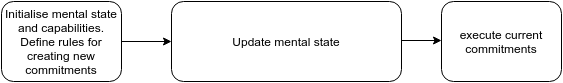
\includegraphics{Agent0Interp.png}
\caption{Agent0 interpreter, adapted from~\cite{DBLP:journals/ai/Shoham93}}
\label{fig:Agent0Interp}
\end{figure} % >>>

Figure~\ref{fig:Agent0Interp} presents the schematic of the Agent0
interpreter. The generic agent interpreter's basic loop contains two steps:
(1)~read the current messages and update the mental state; (2)~execute
commitments (possibly resulting in further belief changes).

Agent0 is a prototype programming language used to illustrate the Agent
Oriented Programming paradigm. It includes only constructs related to the
agent level of a multiagent system. In his proposal, Shoham mentioned that
a society of agents would need further organisation in order to work
properly. He suggested that the roles and norms could be appropriate
options to consider, but there was no concrete implementation for any of
the social level constructs.

A rich profusion of agent oriented programming languages followed Agent0,
focusing, as well, on the mental notions and implying a societal view of
computation.  Many of them are heavily influenced by the Belief, Desire,
Intention agent architecture and by the reactive planning theory.  The
Belief, Desire, Intention agent architecture~\cite{DBLP:conf/icmas/RaoG95},
based on the human practical reasoning theory developed by Bratman in the
mid-1980s~\cite{Bratman:1999}, provides a mechanism to separate the plans
selection from the current plans execution.  The reactive
planning~\cite{DBLP:conf/aaai/GeorgeffL87} represents a group of techniques
used in the process of selecting their actions by autonomous agents.
Notable agent oriented programming languages, from a historical point of
view, are AgentSpeak~\cite{DBLP:conf/maamaw/Rao96}, based on speech acts;
MetateM~\cite{DBLP:conf/promas/Fisher05}, based on temporal logic;
3APL~\cite{DBLP:conf/promas/DastaniRDM03}, based on practical reasoning
rules; Jason~\cite{DBLP:books/sp/map2005/BordiniHV05}, which extends
AgentSpeak with communication; and
GOAL~\cite{DBLP:journals/corr/cs-AI-0207008}, based on declarative goals.

A diversity of language constructs are employed to model the abstract
concepts manipulated in the Agent Oriented Programming paradigm. These
abstract concepts include beliefs, goals, intentions, plans, groups, norms,
interactions, roles, artifacts, percepts, actions, and describe the
individual level, the social level and the environmental level of a
multiagent systems. Not all abstract concepts have a one to one
correspondence with the programming language constructs, and not all of the
language constructs are first-class constructs. The individual (agent) level
had most of the attention so far, with environment coming after, and social
level lagging behind. Only recently the social level of multiagent systems
has started to receive more attention.
\section{Defining Agency} % <<<

Wooldridge and Jennings~\cite{DBLP:journals/ker/WooldridgeJ95} outline the
attributes and characteristics of agents as follows.

"A weak agency has the following attributes:

\begin{itemize}
  \item \textbf{autonomy}: agents operate without the direct intervention
      of humans or others, and have some kind of control over their actions 
      and internal state (Castelfranchi, 1995);
    \item \textbf{social ability}: agents interact with other agents (and
      possibly humans) via some kind of agent-communication language
      (Genesereth and Ketchpel, 1994);
    \item \textbf{reactivity}: agents perceive their environment, (which may
      be the physical world, a user via a graphical user interface, a
      collection of other agents, the INTERNET, or perhaps all of these
      combined), and respond in a timely fashion to changes that occur in it;
    \item \textbf{pro-activeness}: agents do not simply act in response to
      their environment, they are able to exhibit goal-directed behaviour by
      taking the initiative."~\cite{DBLP:journals/ker/WooldridgeJ95}
\end{itemize}

They also identify the characteristics of a strong notion of an agency. The
more specific meaning implies that on top of the properties listed for the
weak agency, the agents have to be \textbf{conceptualised or implemented
using human-like attributes} ~\cite{DBLP:journals/ker/WooldridgeJ95} such
as mentalistic notions (e.g.  knowledge, beliefs, intentions, obligations),
emotional notions or even graphical resemblance.

%\todo{explain how do AF-Raf agents relate to the definitions of weak and
%strong agency}
% >>> >>>
\chapter{Role Theory} % <<<

The Role Theory elaborated in Sociology and Social Psychology tries to
explain the predictability of individual behaviour by linking it to the
social structures. Role Theory uses the theatre metaphor to describe human
behaviour and patterns of interaction; in this context individuals are
viewed as actors enacting a role in a play. There are several approaches to
Role Theory, each with slightly different definitions of roles, but the
common idea is that each role has associated behavioral expectations.
Conformity or nonconformity to these expectations trigger rewards or
punishments. These behavioral expectations can be expressed as rights and
duties, and are guided by social norms.

According to B.J. Biddle~\cite{biddle1986recent} there are five major
approaches to Role Theory: the Functional Role Theory have a static
understanding of roles, which are seen as a set of expectations from society, inflexible and universally agreed upon; In the Interactionist
Perspective interpersonal interaction is of major importance, with roles being
negotiated between individuals on a constant basis; the Structural
Perspective focus more on social structures like the one of status as the
key concept in role definition; Organisational Role Theory looks at the
development of roles in the context of preplanned and task oriented social
systems; The Cognitive Role Theory emphasizes the relationship between
expectations and behaviour.

Role Theory bridges individual behaviour and social structure. Roles as
social constructs which influence individual behaviour on different levels. They
have associated characteristic beliefs and attitudes, meaning that whenever
roles are changing, beliefs and attitudes change along. Roles also specify
goals, tasks and performance standards required in specific social
situations, acting as plans or blueprints to guide behaviour.

An individual plays multiple roles over time, and at the same time. As a
result roles interact not only at the social level, but on an individual
level as well. A number of issues arise from this interaction; on the
negative side this can cause role conflict, role strain, role overload, but
on the positive side it also allows for role accumulation.

In summary, Role Theory could be synthesised as follows: Social situations
are governed by social norms, which determine behavioral
expectations (social roles), which are in turn, described in term of duties
and rights or obligations and permissions. The expectations are both
internal and external to the individual. Conformity results in rewards,
while nonconformity triggers social sanctions. Role prescriptions are
subject to change through social pressure.

During the last 35 years the role metaphor has been applied to many fields
of computer science including to programming languages, software
engineering, coordination languages, databases, multiagent systems,
knowledge representation, formal ontology, computational linguistics,
security, and conceptual modelling~\cite{DBLP:journals/ao/BoellaTV07}.
Unfortunately, there is little consensus between these different approaches,
which makes it very hard to transfer results from one area to another.

The idea of role oriented programming appeared within object
oriented programming.  ObjectTeams~\cite{DBLP:journals/ao/Herrmann07}, and
EpsilonJ~\cite{DBLP:conf/snpd/MonpratarnchaiT08} are examples of such
object oriented programming languages that have explicit support for roles.
A role taxonomy was developed~\cite{graversen06nature} to help role
researchers understand, communicate and spawn new ideas in the
context of object oriented programming.

%\todo{rephrase and add citation} JavaScript natively supports various
%function-based implementations of Role[40] patterns like Traits[41][42] and
%Mixins.[43] Such a function defines additional behavior by at least one
%method bound to the this keyword within its function body. A Role then has
%to be delegated explicitly via call or apply to objects that need to
%feature additional behavior that is not shared via the prototype chain.


The programming language ObjectTeams models roles by specific classes and
defines a playedBy relationship at the class level. This relationship
specifies that each instance of the role class will be permanently attached
to a base instance (the class that the role is decorating). It is possible
to group a number of roles into a team.  Teams combine both
classes and packages. They are classes because they have fields and
methods, and may apply inheritance and are instantiable. They are packages
because they contain a set of classes~\cite{DBLP:journals/ao/Herrmann07}.

In the multiagent systems domain, there have been a number of successful
endeavours to incorporate the concept of role. Examples include
PowerJava~\cite{DBLP:journals/entcs/BaldoniBT06}, an extension of Java, and
ROPE~\cite{DBLP:conf/coopis/BechtGKM99}, a language independent framework.
However, at the present time there is no agent oriented programming language
to have roles built in as first class programming constructs.

In PowerJava~\cite{DBLP:conf/sac/BaldoniBT06} roles are implemented as classes, which can be instantiated only
in the presence of an instance of the player and of an instance of an
institution. The definition of a class implementing a role is included in
the class of the institution the role belongs to. Powers are methods which
can access private fields and methods of the institution they belong to,
and of the other roles of the same institution.
%Rope: role oriented programming environment for multiagent systems. Becht
%1999

%Roles survey. Ekinci >>>
\chapter{Organisational Theory}  % <<<

Organisational Theory is a discipline of social sciences originating over 100
years ago. Organisational Theory studies organisational design, organisational
structures, the relationship between organisations and their environment, and
the behaviour of individuals in organisational settings.

An organisation could be regarded as a coordinated collective action
towards a common goal. Organisations are governed by rules and placed
within an environment.

The study of formal organisations accompanied the Industrial
Revolution, following the need to organise labour. There are a number of
organisational theories that can be categorised in three groups or stages
depending on their main focus: 1) classical theories focus on the product,
2) neoclassic theories focus on the employee, and 3) contemporary theories focus
on the environment~\cite{DohertySD01}.

Each of the Organisational Theories can be described in terms of the four
components of a division of labour: 1) the hierarchy of authority, 2) the
span of control, 3) the level of centralisation versus decentralisation in
decision making, and 4) the specialisation of functions or tasks.

The hierarchy of authority refers to a system of rules regarding the line
of communication and control, which determine the organisational structure.
When you view the organisational structure in relation to the
specialisation of tasks the result is a functional organisation, while
focusing on the "end product" results in a product organisations. Focusing
on both function and product results in a matrix organisation with a dual
authority.

The span of control can be narrow, resulting in a high organisation with
multiple levels, or wide, resulting in a flat organisation with fewer levels.

The centralisation and decentralisation refers to the number of people and
the grade in which people are involved in decision making. In centralised
organisation, the number of people involved in decision making is small,
representing the upper-level in the authority hierarchy. In decentralised
organisations the decision making is delegated to all levels.

Regarding the specialisation, a high degree of specialisation means that
each individual needs to perform fewer smaller and simpler tasks, which have
the advantage of promoting proficiency and the need of less transfer time
between tasks. However,the disadvantage is the resulting dissatisfaction
associated with boredom.

The organisational rules (global constraints and conventions), structures
(role structure) and patterns (describing agent interaction) have been
identified as the most significant organisational components to the
multiagent system development~\cite{DBLP:conf/aose/ZambonelliJW00}.

Within the multiagent systems development settings, a number of
software frameworks and models that promote organisation oriented
programming have been developed. They facilitate the definition
of a social or organisational level on top of the agent level. Examples
include Moise+~\cite{DBLP:conf/atal/HubnerSB02},
Gaia~\cite{DBLP:journals/aamas/WooldridgeJK00},
MASE~\cite{deloach2001analysis}, AALAADDIN~\cite{ferber1998meta}.  

A very recent and slightly different approach is to merge more
technologies. JaCaMo~\cite{DBLP:journals/scp/BoissierBHRS13}, a multiagent programming framework, combines
three different technologies already widely used: 1. Jason, the agent
oriented programming language; 2. Cartago, the framework for programming
environments; and 3. Moise, the organisational model. It advances a new
programming paradigm; the multiagent programming that incorporates all the
principles of programming agents, organisations, environments and
interactions. In order to use this framework you would have to understand
and be proficient in all three technologies.

Recently, a number of normative organisation frameworks were developed,
some of which incorporate programming languages for norm-aware agents and
normative organisation. Some examples are N-2APL and 2OPL.

The N-2APL~\cite{DBLP:conf/aamas/AlechinaDL12} agent oriented programming
language is based on the 2-APL programming language. "N-2APL agents are able
to deliberate on their goals, norms, and sanctions before deciding which
plan to select and execute, and they are able to violate norms if it is in
their overall interest to do so"~\cite{DBLP:conf/atal/DybalovaTDL13}.

2OPL~\cite{DBLP:conf/atal/DybalovaTDL13} is a programming language (logic
based) for developing agent organizations.  2OPL uses the following
abstractions: brute facts, effects of actions, norms and sanction rules.
Brute facts are the state of the multiagent organisation. The state is
represented by the environment.  Transition rules describe how
actions change the brute facts. Norms describe which environment states
represent violations.  Sanction rules can be programmed to respond to norm
violations~\cite{dastani2009programming}. 

It was previously acknowledged that, in programming agent organisations,
developing new organisational abstractions at the programming language
level is the preferred approach in order to reduce the effort needed for
programming and maintaining agent
systems~\cite{DBLP:conf/esaw/RiemsdijkHJ09}.

% >>>
\chapter{Agent Oriented Programming Languages} % <<<
Role Theory and Organisational Theory have not yet been fully exploited at
the programming language level. The three representative agent programming
alnguages most widely in use are
Jason/AgentSpeak~\cite{DBLP:books/sp/map2005/BordiniHV05},
2APL~\cite{DBLP:journals/aamas/Dastani08}, and
GOAL~\cite{DBLP:journals/corr/cs-AI-0207008}. I will look at
the similarities similarities between them, and try to identify the gap
between the established functionality and the desirable functionality of
the agent oriented programming languages that could support a more
structured multiagent interaction. I will include in this analysis some
newly developed programming languages, SimpAl and 2OLP, that are relevant
to this research.

\subsection{Jason/Agent Speak} % <<<
Jason is an interpreter written in Java for an extended version of the
AgentSpeak programming language, it also provides a platform for the
development of multiagent systems. AgentSpeak is logic based and supports
Belief Desire Intention agent architecture. Additionally, the AgentSpeak
agent is a reactive planning system.

The core concepts defining an AgentSpeak agent are the belief base, the
plan library, the goals and the triggering events. The belief base consists
of a set of ground atomic formulae. There are two types of goals in
AgentSpeak: achievement goals and test goals, both of which are written as
atomic formulae prefixed with either "!" or "?". The first one describes a
state of the world to be achieved, while the other specifies a check for
conformity with the agent's belief base. The triggering events can be
either addition or deletion of beliefs and goals. The plan consists of a
head, a context and a body. The head is represented by the triggering
event; the context comprises of a conjunction of beliefs which determine if a
plan is applicable; the body is a sequence of basic actions or
(sub)goals. In order to be executed, plans have to be designated as
intentions. More exactly, intentions represent partially instantiated
plans that were selected for execution.

Additionally, the AgentSpeak interpreter relies on three selection
functions. Firstly, the event selection selects a single event from the set
of events. Second, the option function selects a plan from the set of
applicable plans. And third, the intentions selection function selects an
intention from the set of intentions.

For managing the social level of the multiagent system, Jason can be used
in conjunction with Moise+ organisational framework, combination known as
J-Moise+~\cite{hubner2007j}.

% >>>

\subsection{2APL} % <<<
2APL is also a Belief Desire Intention architecture-based programming
language. 2APL is modular, and integrates both the declarative and the
imperatives style of programming. Also, 2APL incorporates two sets of
programming constructs: the ones that implement multiagent concepts and the
ones that implement individual agent concepts. The multiagent level
constructs include functionality like creating individual agents, external
environments, assigning unique names to agents, and specifying access
relations. The individual agent concepts include beliefs, goals, actions,
plans, events and three types of practical reasoning rules. The beliefs and
goals are implemented in a declarative way to support the reasoning and
updating mechanisms. Plans, external environments, events, flow of control
are implemented in an imperative way.

Environments are implemented as Java objects. Information regarding changes in
the environment can be accessed by the agents in two different ways:
actively through sensors or passively through events. Another distinction
is made between goals and events. Despite both of them triggering agent
action, goals correspond to a desirable state, while the events correspond
to environmental changes.

Different types of actions are available to 2APL agents, such as: updating
beliefs, testing beliefs and goals, managing dynamics of goals, external
actions and communication actions.

The three types of reasoning rules mentioned earlier are: rules that
generate plans to achieve goals, rules that process internal events and
received messages, and rules to handle and repair failed plans.

2APL employs modules to implement the functionality of
roles~\cite{dblp:conf/prima/dastanims08}. We will discuss more about it in
the next chapter.
% >>>

\subsection{GOAL} % <<<
GOAL is a rule-based programming language, its focus is agent reasoning.
GOAL agents consist of four components: a belief base, a goal base, action
rules, and action specifications. An actual GOAL agent program is a set of
modules each consisting of various sections including knowledge, beliefs,
goals, action specifications, and a program section containing action
rules. Each of the sections is represented in a knowledge representation
language such as Prolog~\cite{DBLP:books/daglib/0076175}.

The init module defines the agent's initial mental state. It includes the
knowledge, the initial beliefs, the goals, and the action specifications.
The main module specifies a strategy for selecting actions using action
rules which, in turn, rely on the agent's mental state. The event module
provides rules for processing information received from the environment.
Actions are specified using preconditions and postconditions.

GOAL agents use a blind commitment strategy, meaning that an agent commits
to achieving a goal and only drops it after it has been achieved. GOAL
distinguishes different types of goals: primitive, achievement or achieved
goals~\cite{DBLP:conf/jelia/indriksH08}.

GOAL doesn't manage in an explicit way the social level of the agent system.
% >>>

\subsubsection{SimpAL} % <<<
Ricci  and Santi developed a novel programming language, called
simpAL~\cite{DBLP:conf/oopsla/RicciS11,DBLP:conf/oopsla/RicciS12}, that
supports organisational structure, types and type
checking~\cite{DBLP:conf/promas/RicciS12}. SimpAl draws inspiration from
the Agent and Artifacts model~\cite{DBLP:conf/atal/RicciVO07} and from the
Jason programming language, which is based on the Belief, Desire, Intention
model. SimpAL is conceived as an extension to the Java object oriented
programming language with a separate agent abstraction layer.

Even though this language is very different from AF-Raf, there are a number
of overlapping concepts. SimpAL imports a social view of computation where
agents playing different roles constitute an organisation, and work within
a shared environment. The main building blocks of this model are agents
(autonomous components) and artifacts (the environmental components that
provide functionality or services). The agent has a belief base, some tasks
to perform and a set of plans to utilise in order to accomplish the tasks.

SimpAl roles are similar to AF-Raf roles in that each role is composed of a
set of tasks types, in the same way an AF-Raf role constitutes a set
of operations, where tasks are the analogous to the AF-Raf operations.
However, operations and tasks are completely different entities. An
operation is defined by the type of messages exchanged by the agents, while
a task is defined by a set of parameters and a set of optional attributes
(understand, goal, pre-attributes).

SimpAL roles are organised in a slightly different manner compared to the
AF-Raf's session model. In AF-Raf sessions can be seen as a kind of protocol
prescribing the agent communication. In simpAL organisation models are used
to define organisation types, that bring together related roles and
artifact in coherent units named workspaces. Organisation types are
implemented by concrete organisations. SimpAL organisation types do not put
any constraint on the order in which interactions between agents occur, as
AF-Raf session types do, instead, they simply group together related roles
and artifacts working in a similar way to the object oriented programming
interfaces.

A number of static type checks are performed. At the role level it is
verified that for each task type there exists at least one plan, and for
each plan, it's checked that the type of the sent messages are only the ones
defined in the task type. Assignment of tasks are also checked to
correspond to the task types defined in the role, and that the types of
the messages sent to an agent correspond to that the agent can understand.

Errors about beliefs that are checked include finding, inside the plans,
beliefs that are not declared, and beliefs that are assigned with
expressions of the wrong type.

Similar checks are performed at the environment level. The usage interface
represents the type of artifact, and contains the observable properties and
the operations provided by the artifact. Artifact template is the actual
artifact implementation. On the agent side are checked errors regarding
artifact operations and its observable state. For each action in the plan
there must be a matching operation in the artifact's interface.  Likewise,
for each update belief statement regarding an artifact property there must
exist a matching observable property in the usage interface. On the
environment side, it is checked that the artifact templates match the
corresponding usage interfaces. First, checks are performed to ascertain
that for each operation declared in the interface there exists an
implementation in the template, and for any of the observable properties
in the template there exists a declaration in the corresponding interface
with a compatible type.

At the organisation level it is checked that each workspace, artifact, and
agent types declared in an organisational model are actually implemented in
the implementation of the organisation.
% >>>

\subsection{2OPL} % <<<

2OPL~\cite{DBLP:conf/atal/DybalovaTDL13} is a programming language for
developing agent organizations.  The used abstractions in the language are
brute facts, effects of actions, norms and sanction rules. Brute facts
represent the state of the environment.  Transition rules describe how
actions change the brute facts. Norms describe what constitute a violation.
Sanction rules enforce the prevention of norm violations. 2OPL's
implementation is based on logic programming.

2OPL~\cite{DBLP:conf/atal/DybalovaTDL13} is a normative organization
oriented programming language. It allows the programmer to program
organizations in terms of norms. These norms are represented as logical
rules in the language. An organization programmed with this language acts
between a multi-agent platform and the environment, monitoring every action
performed by the agents on the agent platform and capturing violations and
sanctioning the performers of these violations to organize the overall
behavior of the organization.

% >>>

\subsection{Discussion} % <<<

All of the languages referred to above (Jason/AgentSpeak, 2APL, and GOAL)
have a number of constructs to model the agent level concepts: a belief
base to model agent knowledge, goals that model the agent desires, some
sort of plan or strategy for achieving agent's goals, actions that
result in changes, mechanisms for triggering actions based on the mental
state of the agent, and sensing mechanisms to get information about the changes
in the environment.

The perspective is not as uniform when we consider the social level.
Actually, it is quite the opposite; the approach ranges from employing
modules to implement roles (2APL) to using an external organisational framework
(Jason) to manage the social concepts, or disregarding this aspect
altogether (GOAL).

None of the languages investigated above incorporate, as first order
constructs, any social level concepts, that could support organising agent
interaction.

The social level of multiagent systems is where this research work brings
most of its contributions. AF-Raf is a newly designed agent oriented
programming language, that implements social concepts, like the one of
role, as first order constructs. It draws inspiration from the social
sciences as well as form the functional programming languages and
multiparty session types. AF-Raf is not the only proposal in this sense.
SimpAL~\cite{DBLP:conf/oopsla/RicciS11} is, also, a new programming
language implementing social level construct. Notwithstanding the
similarities, AF-Raf and simpAL have very different approaches, and we will
discuss them further in the related work section of the next chapter.

In comparing the social level approaches we will use the organisational
components identified as being the most significant to the multiagent
systems development: (1) the organisational rules (global constraints and
conventions); the organisational structures (role structure); and (3) the
organisational patterns (describing agent
interaction)~\cite{DBLP:conf/aose/ZambonelliJW00}.

\autoref{tbl:comparison} synthesises the main features of 2APL, Jason,
GOAL, simpAL, 2OPL and AF-Raf related to the social level. In addition, I decided to include one more functionality, type checking, which is important not
only for the social level, but for the entire language as a whole.

\begin{table}
\def\.#1{\rlap{\footnote{#1}}}
\begin{minipage}{\textwidth}\centering
\begin{tabular}{lcccccc}
\toprule
Feature & AF-Raf & 2APL & GOAL & Jason & simpAL & 2OPL\\
\midrule
rules     & - & - & - & -\.{could employ J-Moise+ organisational framework}
& - & +\.{norms and sanction rules}\\
structure
  & +\.{roles, as first order construct}
  & +\.{roles as modules}
  & -
  & -\.{could employ J-Moise+ organisational framework}
  & +\.{roles and organisations, as first order constructs}
  & -\\
patterns
  & +\.{sessions}
  & -
  & -
  & -\.{could employ J-Moise+ organisational framework}
  & -
  & -\\
types
  & +\.{algebraic data types}
  & -
  & -
  & -
  & + 
  & -\\
\bottomrule
\end{tabular}
\caption{Comparison of Features Related to Agent Interaction: Rules,
structure, and patterns refer to the organisational rules, structure, and
patterns defined in~\cite{DBLP:conf/aose/ZambonelliJW00}. Types refer
specifically to the typing of messages.}
\label{tbl:comparison}
\end{minipage}
\end{table}

% >>>
\subsection{Summary} % <<<
So far we've identified two important needs that are not met by the
present functionality of the Agent Oriented Programming languages, to which
we offer suitable solutions:

(1) The need to structure related social behaviour. One way to accomplish
this would be introducing the concept of role as a first order language
construct.

(2) The need to structure agent interactions into patterns. This could be
achieved by employing sessions to model interaction patterns.

To this list, I would like to add one final area that has long been
neglected in the Agent Oriented Programming languages, even though the
other mainstream programming languages have acknowledged its benefits about
three decades ago.

(3) The need of a consistent type system and type checking mechanisms. We
designed a type system that include algebraic data types.


A remarkable thirty year old paper depicts the benefits of having a type
system and type checking: early detection of errors; greater execution-time
efficiency; and making the programs more structured and easier to
read~\cite{DBLP:journals/csur/CardelliW85}.

% >>>
% >>>
\chapter{Functional Languages} % <<<

"Programming in a functional language consists of building definitions and
using the computer to evaluate expressions. The primary role of the
programmer is to construct a function to solve a given problem. This
function, which may involve a number of subsidiary functions, is described
in a notation that obeys normal mathematical principles. The primary role
of the computer is to act as an evaluator or calculator; its job is to
evaluate expressions and print the results. In this respect the computer
acts much like an ordinary pocket calculator. What distinguishes a
functional calculator from the humbler variety is the programmer's ability
to make definitions to increase its power of calculations. Expressions that
contain occurrences of the names of functions defined by the programmer are
evaluated using the given definitions as simplification rules for converting
expressions to printable form."~\cite{bird1988introduction}

The computer evaluates an expression by reducing it to its simplest
equivalent form and displaying the result. The terms evaluation,
simplification and reduction can all be used to describe this
process. In functional languages, an expression is used only to describe a
value, but it is important to distinguish between values and their
representations. There may be many representations for the same value. The
most important kind of value in functional programming is a function value.
Even though we can't display a function value, we can apply a function to
arguments and display the results. The universe of values is partitioned
into organised collections called types. Each type has associated with it
certain operations. It is important that every well-formed expression in a
programming language can be assigned a type.~\cite{bird1988introduction}

\subsubsection{Haskell Type Classes} % <<<

This section reviews Haskell type classes, because they inspire our notion
of `role', and Haskell modules, so that it is clear they are very different
from type classes. We use the basic mathematical concepts of sets and
equality as examples, because we assume the readers are familiar with these.

% modules
%  - small example
%  - information hiding and encapsulation
%    (exact impl may change; but it is ONE)
%  - separate compilation
%  - analogy with Java classes

Haskell has a modular approach to programming. Modular programming implies
separating the programs into independent modules that perform logically
distinct functions. Modules are integrated into programs through
interfaces. An interface define the elements required and provided by the
module. The advantage of modular programming is that it allows one to write
a module having little knowledge of the code in another module, and, also,
it allows modules to be reassembled and replaced without reassembly of the
whole system~\cite{DBLP:journals/cacm/Parnas72a}.

In Haskell, modules are used to control name-spaces and to create abstract
data types. Moreover, a Haskell program can be seen as a collection of
modules, where the main module loads up the other modules. A module
contains functions, types and type classes that are related and serve a
common purpose.

Haskell modules are often used to implement abstract data types such as
sets.  To illustrate the main features of modules, the code in
Figure~\ref{fig:haskell} is contrived.  The module \textit{Set} contains
the type~$T$ and the functions \textit{add}, \textit{has}, and
\textit{sub}. The \textbf{module} line hides \textit{sub} by not mentioning
it. The names and types of the exported functions \textit{add} and
\textit{has} are visible from outside the module, but their
implementations, which are to the right of~$=$, are hidden.  Similarly, the
type name~$T$ is visible from outside, but the value constructor~$V$ is
not. For example, the set $\{1,2\}$ may be represented by the value
$V[2,1,2]$, but this is not known to the users of the module \textit{Set}.
The names and types visible from outside constitute the module's
\emph{interface}.

\begin{figure}\footnotesize % <<<
\begin{verbatim}
-- built-in and standard library
class Eq b where
  eq :: b -> b -> Bool
instance Eq Int where ...
elem x [] = False
elem x (y:ys) = eq x y || elem x ys
all p [] = True
all p (x:xs) = p x && all p xs

-- file set.hs
module Set (T, add, has) where
  data T a = V [a]
  add (V s) x = V (x:s)
  has (V s) x = elem x s
  sub (V s) t = all (has t) s

  instance Eq a => Eq (T a) where
    eq s t = sub s t && sub t s
\end{verbatim}
\caption{Haskell type class \textit{Eq} and module \textit{Set}}
\label{fig:haskell}
\end{figure} % >>>

% type classes
%  - continue example
%  - ad-hoc polymorphism: multiple implementations with the same interface
%  - analogy with Java interfaces

The type class \textit{Eq} contains types whose values can be compared for
equality. To make a type belong to the class \textit{Eq} one must write an
instance declaration that provides an implementation for a function
named~$eq$. The \textbf{instance} declaration in module \textit{Set} says
that the type constructor~$T$ transforms members of \textit{Eq} into
members of \textit{Eq}. For example, $T(T\,\mathit{Int})$ is in \textit{Eq}
because \textit{Int} is in~\textit{Eq}.

In general, modules are responsible with information
hiding~\cite{DBLP:journals/cacm/Parnas72a} and encapsulation.  On the other
hand, type classes are an elegant mechanism to provide ad-hoc polymorphism,
also known as overloading~\cite{DBLP:conf/popl/WadlerB89}: The same name
refers to different implementations depending on the context.

A type class defines a set of methods that can be used with types that are
members of the class. When you declare an instance of that type class
you have to provide an implementation for all the methods associated with
that class. Haskell type classes are similar to generic interfaces in Java.

Just as Haskell type classes are different from Haskell modules, the roles
we introduce are different from existing 2APL
modules~\cite{dblp:conf/prima/dastanims08}.
% >>>
%\todo{how is this chapter related to one of my objectives}
% >>>
\chapter{Types} % <<<
\subsection{Multi-Sorted Predicate Logic} \label{sec:multi-sorted} % <<<

The starting point in designing a type system is the observation that most
agent oriented programming languages use first order logic, more
specifically predicate logic terms, to represent beliefs and messages. As a
consequence we should look at how the introduction of types is managed in
mathematical logic, and recall basic notions necessary to our
understanding. And, also, introduce notational conventions used in AF-Raf.
Moreover, although these notions are simple, their definitions in
literature tend to have subtle but important differences.

A \emph{term} is a variable, or a function applied to other terms.
\begin{align}
\mathit{Term}\quad\tau &::= \omega \mid \phi \\
\mathit{Variable}\quad\omega &::= \nu \\
\mathit{Function}\quad\phi &::= \nu(\tau_1,\ldots,\tau_n) \\
\mathit{Name}\quad\nu
\end{align}
In AF-Raf, term names are strings.  Because term names uniquely identify a
variable or a function we will say ``the function~$\nu$'' rather than ``the
function with name~$\nu$.'' A term not containing variables is said to be
\emph{ground}.

\begin{remark}
Ground terms are essentially trees of strings.
\end{remark}

A multi-sorted logic has a set~$S$ of sorts.  We use the letter~$\sigma$ to
denote sorts.
\begin{align}
\sigma, \sigma_1, \sigma_2, \sigma_3, \ldots &\in S
\end{align}
Each function~$\nu$ has a signature
$(\sigma_1\times\cdots\times\sigma_n)\to\sigma$.  Function~$\nu$ is always
applied to $n$~terms whose sorts must be, respectively,
$\sigma_1$,~$\sigma_2$, \dots,~$\sigma_n$, and the resulting term has
sort~$\sigma$. We say that $\nu$~has \emph{arity}~$n$. \emph{Constants} are
functions with arity~$0$.

Typically, in mathematical logic, the set~$S$ of sorts and the function
signatures are required to satisfy further constraints. \textit{Bool} must
be one of the sorts. \emph{Formulas} are terms with sort \textit{Bool}.
The argument sorts ($\sigma_1$,~$\sigma_2$, \dots,~$\sigma_n$) either are
all \textit{Bool}, or none is \textit{Bool}.  If the argument sorts are
\textit{Bool}, then the result sort~$\sigma$ must also be \textit{Bool},
and $\nu$ is said to be a \emph{boolean connective}.  If the argument sorts
are not \textit{Bool} and the result sort~$\sigma$ is \textit{Bool}, then
$\nu$ is said to be a \emph{predicate}.  Agent~Factory has these
constraints and AF-Raf inherits them. In addition, AF-Raf uses an infix
notation (described later) for boolean connectives, letter strings starting
with uppercase for predicate names, and letter strings starting with
lowercase for other function names and for variable names.

\begin{remark}
%\rg{I'm not sure about this remark. I think \emph{traditional} logicians
%behave as described here.}
The definitions given here are in-between what applied computer scientists
tend to prefer and what pure logicians tend to prefer.  Computer scientists
work with \emph{expressions} (rather than terms and formulas) and do not
have constraints on function signatures with respect to booleans.
Logicians, on the other hand, do have these constraints and, moreover,
define terms in such a way that formulas are not terms, and predicates are
not functions. Moreover, logicians single out equality between terms as
being a special predicate.
\end{remark}

%\rg{Maybe add some simple examples early on.}
% >>>
\subsection{Algebraic Data Types} % <<<

Algebraic data types offer an alternative way of defining sets of ground
terms. In multi-sorted predicate logic, the sort~$\sigma$ determines a set
of ground terms, namely those of the form $\nu(*)$, where $\nu$ has a
signature of the form $*\to\sigma$.  For example, the sort \textit{Bool}
determines the set of terms that are formulas.  With algebraic data types,
a type~$\delta$ is defined by a sequence of patterns, each of the form
$\nu(\delta_1,\ldots,\delta_n)$. For example, one could define the types
\textit{nat}, $e$, and~$o$ as follows.
\begin{align}
&\mathbf{type}\,\mathit{nat} =
      \mathit{zero}()
  \mid\mathit{succ}(\mathit{nat})
  \mid\mathit{add}(\mathit{nat},\mathit{nat}) \\
&\mathbf{type}\,e =
      \mathit{zero}()
  \mid\mathit{succ}(o)
  \mid\mathit{add}(e,e)
  \mid\mathit{add}(o,o) \\
&\mathbf{type}\,o =
      \mathit{succ}(e)
  \mid\mathit{add}(o,e)
  \mid\mathit{add}(e,o)
\end{align}
%\rg{These things are presented as if they are completely standard. They're
%not. I think they should be presented as part of the design of AF-RAF.}
We make the following observations.
\begin{enumerate}
\item
  Function names may appear in multiple definitions. For example,
  \textit{zero} appears in the definition of~$\mathit{nat}$ and also in the
  definition of~$e$. In particular, the term $\mathit{zero}()$ belongs both
  to the set of ground terms defined by the type~$\mathit{nat}$ and to the
  one defined by the type~$e$.
\item
  Function names may appear multiple times in the same definition. For
  example, \textit{add} appears twice in the definition of~$e$. (This
  property distinguishes our types from polymorphic
  variants~\cite{garrigue1998}.)
\item
  Type definitions may be recursive or mutually recursive. For example,
  $\mathit{nat}$~appears within the definition of~$\mathit{nat}$.
\end{enumerate}
The set of ground terms corresponding to type~$\mathit{nat}$ is the following.
\begin{equation}
\begin{aligned}
\{\,&\mathit{zero}(), \\
    &\mathit{succ}(\mathit{zero}()),
        \mathit{succ}(\mathit{succ}(\mathit{zero}())), \ldots \\
    &\mathit{add}(\mathit{zero}(), \mathit{zero}()),
        \mathit{add}(\mathit{zero}(), \mathit{succ}(\mathit{zero}())),
        \ldots \\
    &\mathit{succ}(\mathit{add}(\mathit{zero}(), \mathit{zero}())),
        \ldots \\
    &\ldots\, \}
\end{aligned}
\end{equation}
Moreover, $e$~and~$o$ partition~$\mathit{nat}$.

\begin{proposition}
Algebraic data types (as defined above) are strictly more expressive than
sorts. More precisely, (1)~all sets of ground terms that can be defined by
sorts can also be defined by algebraic data types, and (2)~there are pairs
of sets of ground terms that can be defined by algebraic data types but
cannot be defined by sorts.
\end{proposition}

\begin{proof}
For~(1), we define a type~$\delta(\sigma)$ for each sort~$\sigma$ as
follows: For each function $\nu:(\sigma_1,\ldots,\sigma_n)\to\sigma$ we add
a pattern $\nu(\delta(\sigma_1),\ldots,\delta(\sigma_n))$to the definition
of type~$\delta(\sigma)$. It is easy to see, by structural induction, that
the sort~$\sigma$ and the type~$\delta(\sigma)$ define the same sets of
ground terms.

For~(2), note that, given a fixed set of function signatures, the sets of
ground terms defined by distinct sorts are disjoint. In the previous
example, however, the sets of ground terms defined by the types
$\mathit{nat}$~and~$e$ have (at least) a common element, namely
$\mathit{zero}()$.
\end{proof}

Finally, let us note that there are sets of ground terms for which it is
undecidable whether a given term is an element.  (A classic result of
computability theory is that there are undecidable sets of bit-strings, and
sorted ground terms can encode bit-strings.) In particular, there exist
sets of ground terms that cannot be defined using algebraic data types.
%\rg{These things are probably too cryptic, and should be explained more.}

% >>>

%\todo{how is this chapter related to one of my objectives}
% >>>
\chapter{Multiparty Session Types} % <<<

The next research area we draw inspiration from is the area of multiparty
session types, developed at the intersection of communications systems and
type theory. Multiparty session types represent a type systems that ensure
communication safety among two or more participants. This is achieved by
the global types, which can be viewed as a global specification of the
participants' actions, or, in other words a global specification of the
interaction protocol. The global types are projected at the level of each
participant as local types. The programs are eventually type checked
against the local types~\cite{DBLP:journals/jacm/HondaYC16}.

The research in session types initiated in process calculi and programming
languages for binary session, was extended to multiparty asynchronous
session types. In binary session types, where you have just two
participants, the local type serves as the description of the whole
conversation as well, but for multiparty sessions the whole conversation
can't be specified without the type abstraction which describes global
conversation scenarios of multiparty sessions.~\cite{DBLP:journals/jacm/HondaYC16}

A session is a series of interactions which serve as a unit of
communication. The structure of a session is abstracted as a type. Such a
global type is like a shared agreement among communication peers, and
represents the basis for efficient type checking through its projection
onto individual peers.

{\def\l#1->#2:#3<#4>{\mathtt{#1}\to\mathtt{#2}:#3\langle\mathsf{#4}\rangle}

Here is an example of such a type from
Honda et al.~\cite{dblp:conf/popl/hondayc08}:\\
  $\mu\mathbf{t}.$
  $\l DP->K:d<bool>. $\\
  $\l KP->K:k<bool>. $\\
  $\l K->C:c<bool>.\mathbf{t}$

This type means that process \texttt{K} receives two booleans, one from
\texttt{DP} through channel~$d$ and one from \texttt{KP} through channel~$k$,
then sends a boolean to~\texttt{C} through channel~$c$, and the whole process
repeats.

\begin{figure}\footnotesize % <<<
\begin{center}
\begin{tabular}{llcll}
  Global & $G$ & $::=$ & $p \to p' : k\langle U\rangle.G'$ & values
  \\  && $\mid$ & $p\to p' : k \{l_j : G_j\}_{j\in J}$  & branching
  \\ && $\mid$  & $G,G'$ & parallel
  \\ && $\mid$ & $\mu {\bf t}. G$ & recursive
  \\ && $\mid$ & ${\bf t}$ & variable
  \\ && $\mid$ & ${\sf end}$ & end
\\
Value & $U$ & $::=$ & $\tilde S \mid T@p$
\\
Sort & $S$ & $::=$ & ${\sf bool}\mid {\sf nat}\mid\ldots\mid\langle G\rangle$
\end{tabular}
\end{center}
\caption{Syntax of Global Types~\cite{DBLP:journals/jacm/HondaYC16}}
\label{fig:globalType}
\end{figure} % >>>

The grammar of global session type, or global type, denoted by $G$,$G'$,...
is given in \ref{fig:globalType}. Type $p \to p' : k\langle U\rangle.G'$
says that participant $p$ sends a message of type $U$ to channel $k$, is
received by participant $p'$, and interactions described in $G'$ takes
place. Type $p\to p' : k \{l_j : G_j\}_{j\in J}$ says participant $p$ sends
one of the labels to channel $k$ which is then received by participant $p$.
If $l_j$ is sent, interactions described in $G_j$ take place.  Type $G,G'$
represents concurrent run of interactions specified by $G$ and $G'$ . Type
$μt.G$ is a recursive type for recurring conversation structures~\cite{DBLP:journals/jacm/HondaYC16}.


%\begin{figure}\footnotesize % <<<
%\begin{verbatim}
%Value U ::= S˜ | T@p
%Sort S ::= bool | ... | G
%Local T ::= k!UT send
%          | k? UT receive
%          | k⊕ {li : Ti}i∈I selection
%          | k&{li : Ti}i∈I branching
%          | μt.T | t | end
%\end{verbatim}
%\caption{Syntax of Local Types}
%\label{fig:localType}
%\end{figure} % >>>
%The grammar is given in~\ref{fig:localType}.

Local session types or local types, ranged over by $T$,$T'$ are types for
local behaviour of processes, acting as a link between global types and
processes. The following rules define how the projection is performed from the global type to the local types of each participant. The value global type is
projected either as a send local type or as a receive local type. The
branching global type is projected as either a selection (describes the
behaviour of selecting from a number of options) or a branching (describes
the behaviour of waiting for an option to be selected) local type~\cite{DBLP:journals/jacm/HondaYC16}.

\cite{DBLP:journals/jacm/HondaYC16} describes the Programming Methodology
for Multiparty Interactions as follows: "Once given global types as our
tool, we can consider the following development steps for programs with
multiparty sessions.  Step 1 A programmer describes an intended interaction
scenario as global type G, and checks that it is linear.  Step 2 She
develops code, one for each participant, incrementally validating its
conformance to the projection of G onto each participant by efficient
type-checking.  When programs are executed, their interactions are
guaranteed to follow the stipulated scenario. The type specification also
serves as a basis for maintenance and upgrade."

% >>>
\chapter{Agent Factory} % <<<

Agent Factory~\cite{collier2002agent} \cite{russell2011af} is an
open-source Java-based development framework that provides support for the
development and deployment of agent-oriented applications.

Agent Factory provides a generic run-time environment for deploying
agent-based systems that is based on the FIPA
standards~\cite{poslad2000fipa}.  Central to this environment is one or
more configurable agent platforms that support the concurrent deployment of
heterogeneous agent types that make up an application, and which can employ
a range of agent architectures and interpreters. In other words the agents
can be categorised in two subgroups: the Application Agents and the System
Agents. The Application Agents implement the application logic. The System
Agents provide the services infrastructure needed to support the deployment
of Application Agents.

Platform-level resources in the form of platform services are shared
amongst agents. The default platform services are: Agent management
services, which provides support for creating, terminating, suspending and
resuming agents; and local message transport service, which provide an
intra-platform communication channel. Other platform services include the
HTTP message transport service and the directory facilitator service.

Agent Factory also offers monitoring and inspection tools that aid the
developer in debugging their implementations.

Another key feature of Agent Factory is the Common Language Framework,
which represents a collection of pre-written components that facilitates
the design and implementation of diverse Agent Programming Languages in
Agent Factory\null. The Common Language Framework includes a generic logic
framework, a framework for planning and for executing plans, a common API
model based on sensors, actions and modules, an outline grammar and
template compiler implementation based on JavaCC, and a configurable
debugging tool.

The Common Language Framework supports the building of agent interpreters
on top of the Agent Factory core. These interpreters operate within an
agent platform to control the execution of the agent according to an
interpreted Agent Oriented Programming language. This way agents written in
different languages share the same actions, sensors and modules (libraries
or APIs). Actions, sensors and modules are written in Java, and they extend
the agent program so that it can get information about its environment and
act out its intentions. Actions are used to produce changes to the
environment, while sensors generate beliefs, and change the knowledge of
the agent. Each action has an interface that defines how it may be invoked
from within the agent program. If a set of actions and sensors are linked
together they can be defined within a module. A module may also provide
resources that are shared amongst several sensors and actions.

There are four Agent Programming Languages that have been integrated with
Agent Factory using the Common Language Framework: \begin{enumerate}

\item \textit{AFAPL}, a reimplementation of the original Agent Factory
agent programming language that is based on commitment rules;

\item \textit{AF-AgentSpeak}, an implementation of the AgentSpeak language based on Jason;

\item \textit{AF-TeleoReactive}, an implementation of Nilsson's teleo-reactive
programming model;

\item and the new \textit{AF-Raf} programming language, that draws
inspiration from functional languages .
\end{enumerate}

Agent Factory is fully integrated with Eclipse in a way that simplifies
the task of providing support for new languages and architectures.

For further details on Agent Factory the reader is directed
to~\cite{collier2009modeling}. The Common Language Framework is described
in~\cite{russell2011af}. Also, a discussion on the evolution of Agent
Factory since it was created in the early 1990s can be found
in~\cite{muldoon2009towards}.
% >>>

%>>>

\part{AF-Raf Agent Oriented Programming Language}\label{part:AF-Raf} % <<<
\chapter{Main AF-Raf Concepts}\label{ch:concepts} % <<<

%\todo{1. Develop an example bit by bit by adding functionality. 2. Describe
%the thought process of designing the program. 3. Add diagram to Agent
%Factory. 4. Move calculator example to case study. 5. Add discussion to the
%comparison with other work.}

\section{An overview of the AF-Raf programming Language} % <<<

AF-Raf is a new agent oriented programming language specifically developed
to incorporate the support for organising multiagent systems at the
language level. AF-Raf programming language is integrated with the
Agent Factory development framework, which provides support for the
development and deployment of agent-based systems.

The main particularity of AF-Raf, that makes it unique among agent oriented
programming languages is that, even though it is built upon the agent
oriented conceptual framework, it also draws inspiration from functional
languages.

\begin{figure}\footnotesize % <<<
\begin{verbatim}
include stdio

rule State(initialized()) & Name(n) {
      println("hello from " + n);
}

rule Monitoring(name, addr) {
      println("ask " + name + " for status");
      send(agentID(name, addr), request(status()));
}

rule Message(other, status(alive())) {
      println("OK, ask again.");
      send(other, request(status()));
}

rule Message(other, status()) {
      println("Oh, someone wants me alive!");
      send(other, inform(status(alive())));
}
\end{verbatim}
\caption{The code of an AF-Raf agent}
\label{fig:AF-Raf}
\end{figure} % >>>

The AF-Raf core concepts include: beliefs, rules, actions, sensors, roles,
sessions, and types. They are related to one another and the unique
features of AF-Raf are built upon them. Among these concepts, the ones of
roles, sessions and types, constitute new approaches and they will be
described in more depth in the sections to follow. Figure~\ref{fig:AF-Raf}
illustrates a simple AF-Raf agent.

\begin{figure}\footnotesize % <<<
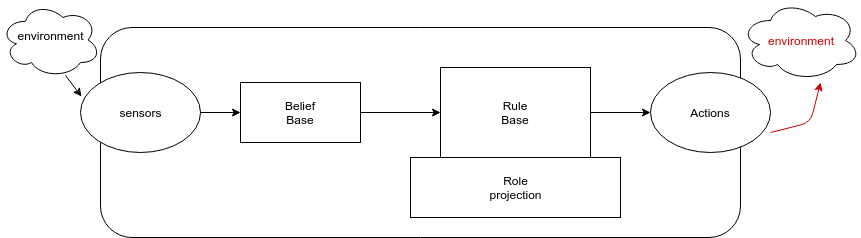
\includegraphics{AF-RafArchitecture2.png}
\caption{AF-Raf agent architecture}
\label{fig:AF-RafArch}
\end{figure} % >>>

The first two fundamental components of AF-Raf are the \textit{belief base}
and the \textit{rule base}. The belief base models the agent's view of the
current state of its environment and the rule base models the agent's
behaviour. Figure~\ref{fig:AF-RafArch} presents the AF-Raf agent
architecture.

Beliefs in AF-Raf are regarded as logical terms and represented in the form
of trees of strings. Beliefs are grouped together in a belief base that can
be accessed by and updated by the agent. On the other hand, rules
represent a means for accessing the belief base and also a way of
triggering agent behaviour. Figure~\ref{fig:rule} illustrates a simple
AF-Raf rule, where $status()$ and $request(status())$ represent AF-Raf
beliefs.

A rule has two main components besides a name, which is optional. These
components are a query and an action. The query is like a condition that
has to be met and can be seen as a question sent to the belief base. If the
belief base is meeting the condition then some action is triggered. The
rules are evaluated at each time-step. The first stage of evaluating a rule
is to evaluate the query on the current belief base. The result is a set of
query results that represent matchings. If the set is not empty, the
action is then evaluated for every matching. There is no particular order
in which the matchings are evaluated. 

Each of the matchings from the set of query results indicates what term
to substitute each free variable in the action. In other words, a matching
is a set of bindings that covers all the free variables in the action (of
the rule). The first step of evaluating the action is to apply these
substitutions. The next step is to execute it.

Executing an action means executing a piece of associated Java code.
%Examples of actions include sending a message (\textit{send}) and logging a
%string (\textit{println}).
An action represents the actual agent's behaviour which can
range from printing something to the console, to sending a message to
another agent, creating another agent, or even updating the belief base.
Another way to update the belief base is through sensors.

Sensors are pieces of Java code that are run at each time-step. They are
typically used to update the belief base according to the changes in the
environment. For example, there is a standard sensor (defined in
\texttt{stdio}) that adds a belief $\mathit{Message}(s,c)$ when a message
with content~$c$ is received from sender~$s$.

%Sensors can range from the monitoring of the agent's message inbox to
%monitoring changes in the agent's environment.

% modules
%  - small example
%  - information hiding and encapsulation
%    (exact impl may change; but it is ONE)
%  - separate compilation
%  - analogy with Java classes

\begin{figure}\footnotesize % <<<
\begin{verbatim}
rule Monitoring(name, addr) {
      println("ask " + name + " for status");
      send(agentID(name, addr), request(status()));
}
\end{verbatim}
\caption{AF-Raf rules example}
\label{fig:rule}
\end{figure} % >>>

Actions and sensors are pieces of Java code used to extend the AF-Raf
programs. Actions are invoked within rules. There are a number of actions
included in the standard library, which any agent can use, and there is also
the option to create new actions. Sensors are run automatically at every time
step. Figure~\ref{fig:actions-sensors} presents some of the AF-Raf standard
actions and sensors. Both {\sf println} and {\sf send} actions have been
used in the rule illustrated in \autoref{fig:rule}.


\begin{figure}\footnotesize % <<<
\begin{verbatim}
action println(s) =
          com.agentfactory.raf.RafStandardAction$Println;

action send(agentID(name, address), message) =
             com.agentfactory.raf.RafStandardAction$Send;

sensor com.agentfactory.raf.RafStandardSensor$Message;
\end{verbatim}
\caption{Standard actions and sensors}
\label{fig:actions-sensors}
\end{figure} % >>>


An operation can be defined as a specific kind of rule stating that upon
receiving a message of a particular type, the agent should reply with a
message of a specified type. The message type can be any type including the
type unit(), and in this case there is no actual message returned. Even
though operations can be written as rules, using syntactic sugar to
automatise the process of message passing makes answering messages much
easier.

A role's purpose is to group together related behaviour. As stated before
AF-Raf agents interact through message passing. AF-Raf's role concept
reflects this by considering only those kind of behaviours (rules) that
impact other agents through message passing, namely operations. A role is a
set of operation types, acting in a similar way to interfaces in object
oriented programming. When an agent plays a role it needs to give an
implementation to all the operations defined within that role.

Sessions organise the interaction between agents stating the exact order in
which the messages should succeed. A session brings together related roles
and maps the set of operations defined in those roles to a particular
protocol of conversation. A session specifies the agents involved in the
conversation, as well as the roles they play, then provides a list
containing entries of the form: message type followed by the sender agent
and the receiver agent.

\begin{figure}\footnotesize % <<<
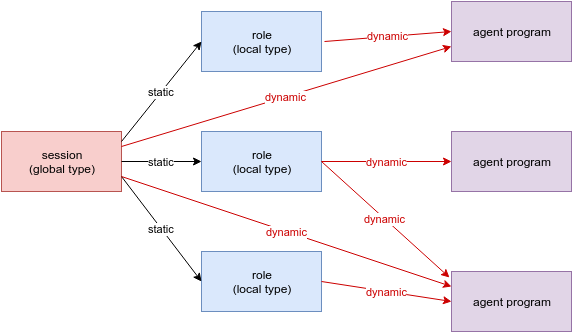
\includegraphics{typechecking.png}
\caption{Type checking in AF-Raf}
\label{fig:typechecking}
\end{figure} % >>>

Figure~\ref{fig:typechecking} illustrates the AF-Raf type checking
functionality.

AF-Raf statically checks that the type of each call message in a session
corresponds to an operation defined in the receiver's role, and each return
message corresponds to an operation defined in the sender's role.

AF-Raf checks dynamically that the agent playing a role actually implements
the specified types of the operations defined in that role.  For each call
message there's an associated call id which must appear in the return
message. This is a way of keeping track of the message pair associated to
an operation and enable the dynamic check that the message types correspond
to the ones defined inside the role. If the types do not correspond an
error is raised.

Further checks are performed at runtime. Each session has a session id.
Each message has to contain the session id so that it can be associated to
an specific session. This enables the interpreter to monitor that the
messages succeed in the right order.

AF-Raf uses Agent Factory as a platform. 
% >>>
\section{The Belief Base} % <<<

In most agent-oriented programming languages, agents maintain a
\emph{belief base}.  The operations available to the agent are
\textit{query} and \textit{adopt}.  A query asks the belief base which
beliefs that follow a certain pattern it holds.  The adopt operation
changes the state of the belief base by adding and possibly removing
beliefs.  Sometimes, the {\it adopt\/} operation comes in two flavours:
{\it update\/} and {\it revise}.  An update corresponds to a change in the
environment, while a revision is exclusively a mental state change.

\subsubsection{Beliefs}

In general, beliefs are sentences in some logic.  However, the focus of
this work is on roles and organisations, not on beliefs.  Thus, AF-Raf uses
a very simple language for beliefs\,---\,they are essentially trees whose
nodes are labeled by strings: \begin{align} \tau &::= \nu(\tau,\ldots,\tau)
&& \text{function term} \\ \nu  &::= {\rm string} &&\text{function symbol}
\end{align} The number of arguments can be any non-negative integer.

Beliefs are ground predicate formulas. That means they do not contain any
free variables.

\begin{example}
The following are AF-Raf \emph{beliefs}:
\begin{align}
&{\it HasColor}({\it my}({\it car}()), {\it blue}()) \\
&{\it IHave}({\it cat}(), {\it int}({\it 10}()))
\end{align}
Note that any belief must contain a function with $0$~arguments, such as
{\it car}, {\it blue}, {\it cat}, and {\it 10\/} in this example;
otherwise, the belief would not have a finite size.  Note also that
function symbols can represent both values (such as~{\it 10\/}) and typing
information (such as~{\it int\/}).
\end{example}

Each function symbol is used with a fixed number of arguments.  For
example, if the function symbol ${\it car}$ is used in one belief with
$0$~arguments in the function term ${\it car}()$, then we expect {\it
car\/} to never have arguments.  We say that each function symbol has an
\emph{arity}, which is~$0$ for {\it car}.  The function terms of arity~$0$,
such as ${\it 10}()$ and ${\it car}()$, are said to be \emph{constants}.

\begin{remark}
Of course, it is important what beliefs mean, not only how they are
represented syntactically.  The meaning of beliefs arises from how beliefs
are used by agents.  We will see later how beliefs trigger actions via
rules, and how beliefs spread through messages.
\end{remark}

\subsubsection{Queries}

In general, a query $q$ is a sentence in some logic that determines a
subset of beliefs.  Given a belief base and a query, it is important to be
able to efficiently find the subset of beliefs from the belief base that
satisfy the query.  Again, AF-Raf takes a simple approach, because its
focus is not the belief base.  Each query is predicate formula, in other
words a term that may contain variables, which are interpreted as patterns.

\begin{align} \tau &::=
\nu(\tau,\ldots,\tau) && \text{function term} \\ \tau &::= x &&
\text{variable term} \\ \nu  &::= {\rm string} &&\text{function symbol} \\
x &::= {\rm string} && \text{variable symbol} \end{align} 

The grammar rules (3.5) and (3.7) are the same as for beliefs.  Thus, any
belief can be used as a query:  It stands for asking whether the belief
base contains that particular belief.

\begin{example} The following are AF-Raf \emph{queries}: \begin{align}
&{\it HasColor}({\it my}({\it car}()), x) \label{eq:query.1} \\ &{\it
HasColor}(y, z) \label{eq:query.2} \end{align} The variables $x$,~$y$,
and~$z$ are easily identifiable, because they are not followed by
parentheses.  Suppose the belief base contains exactly one belief, namely
\begin{align} &{\it HasColor}({\it sky}(), {\it blue}()) \label{eq:skyblue}
\end{align} Belief~\eqref{eq:skyblue} does not match
query~\eqref{eq:query.1} but does match~\eqref{eq:query.2}.  In the latter
case, the match is justified by setting $y$ to be ${\it sky}()$, and
setting $z$ to be ${\it blue}()$.
\end{example}

The previous example shows how a belief matching a query can be described
by a binding of terms, such as ${\it sky}()$ and ${\it blue}()$, to
variables, such as $y$~and~$z$.  More formally, a \emph{match} is a finite
partial map from the set of variables to the set of ground terms.  We write
$[\tau_1/x_1,\ldots,\tau_n/x_n]$ for the match that binds $x_k$
to~$\tau_k$, for all $1\le k\le n$.  Also, we write
$\tau[\tau_1/x_1,\ldots,\tau_n/x_n]$ for the result of substituting in
parallel $x_k$ with~$\tau_k$, for all $1\le k\le n$.

\begin{example} Consider the following belief base \begin{align} &{\it
Knows}({\it john}(), {\it john}()) \\ &{\it Knows}({\it john}(), {\it
laura}()) \end{align} and the following queries \begin{align} &{\it
Knows}(x, y) \\ &{\it Knows}(x, x) \\ &{\it Knows}({\it laura}(), {\it
john}()) \\ &{\it Knows}({\it john}(), {\it laura}()) \end{align} The
results of these queries are, respectively, the following sets of
matchings: \begin{align} &\bigl\{ [{\it john}()/x, {\it john}()/y],\; [{\it
john}()/x,{\it laura}()/y] \bigr\} \\ &\bigl\{ [{\it john}()/x] \bigr\} \\
&\bigl\{\bigr\} \\ &\bigl\{[]\bigr\} \end{align} Note that a variable may
appear multiple times in a query.  In such a case, it implicitly requires
the corresponding subterms to be equal.  Also note that the \emph{empty
match} differs from \emph{no match}.
\end{example}

%\todo{Conjunctive queries.}

\subsubsection{Updates and Revisions}

In general, belief bases have internal and external consistency
requirements.  Internally, beliefs should not contradict each-other.
Externally, beliefs should correspond to reality.

In AF-Raf, the situation is simple: There is no other meaning for beliefs
apart from how they affect the behaviour of the agent, through rules.
Thus, it is the agent's responsibility to detect inconsistencies.  In other
words, inconsistencies are detected by programs, not by the programming
language.

\begin{example} Suppose that a particular agent-oriented program makes the
convention that ${\it not}(x)$ means that `I do not hold belief~$x$'.  In
this case, the query ${\it not}(x)\&x$ detects inconsistencies.  The action
that the agent takes when it discovers an inconsistency could be to report
an error, but may be any action at all.  \end{example}

Similarly, the agent (and not the programming language) is responsible with
ensuring that its beliefs are consistent with the environment.

Once semantic concerns are left to the user program, the programming
language AF-Raf is free to adopt simple mechanisms for updating the belief
base.  The belief base is a set of beliefs, and its operations are those of
a set:  ${\bf adopt}(x)$ inserts belief~$x$ into the belief base, and ${\bf
forget}(x)$ removes the belief~$x$ from the belief base.  In case $x$~is
not a belief, ${\bf forget}(x)$ does not modify the belief base.

% >>>
\section{Types}\label{sec:types} % <<<

AF-Raf contributes to the AOP languages domain by being the first agent
oriented programming language to introduce algebraic data types and
type-checking. From a practical point of view, it tries to improve
upon the following scenario.

\paragraph{Bad Scenario.}

%\rg{Needs a diagram; otherwise, hard to follow.}
Agent~$a$ sends message $\tau_{ab}$ to agent~$b$. Agent~$b$ stores a
subterm~$\tau_b$ of~$\tau_{ab}$ into its belief base. Later, when some
other condition is satisfied, agent~$b$ extracts a subterm~$\tau_{bc}$ of
term~$\tau_b$ and sends it to agent~$c$. Agent~$c$ extracts a
subterm~$\tau_c$ of term~$\tau_{bc}$ and stores it in its belief base.
Later, when some other condition is satisfied, agent~$c$ extracts a
subterm~$\tau$ of~$\tau_c$. Agent~$c$ expects $\tau$ to be an integer
literal, but instead $\tau$ is a string literal. Agent~$c$ notices the
problem, but many things happened since agent~$a$ sent an invalid message.

The goal of AF-Raf's dynamic typing is to notice such errors early.

For this purpose, each agent~$a$ has two attached types. The type $\delta_b(a)$
represents the type of $a$'s beliefs and the type $\delta_m(a)$ represents the
type of messages that $a$ can process. These types are selected when the agent
is created.

Whenever a belief $\tau$ is added to $a$'s belief base, Agent~Factory checks
whether that belief is in the set of terms defined by the $a$'s belief type;
that is, the expression $\tau:\delta_b(a)$ is evaluated.  Whenever a
message~$\tau$ is sent to agent~$a$, the expression $\tau:\delta_m(a)$ is
evaluated, to check whether that message complies to the type of messages that
agent~$a$ can process. In order to send a message to agent~$a$, the other agent
needs the agent identifier of agent~$a$. Agent identifiers typically consist of
a name and an IP address. To support the check for messages we add
$\delta_m(a)$ to the agent identifier of agent~$a$.


\subsection{Algebraic Data Types} % <<<

In AF-Raf, a \emph{belief} is a boolean ground term; in AF-Raf, a
\emph{message} is a non-boolean ground term.

Algebraic data types offer an alternative way of defining sets of ground
terms. In multi-sorted predicate logic, the sort~$\sigma$ determines a set
of ground terms, namely those of the form $\nu(*)$, where $\nu$ has a
signature of the form $*\to\sigma$.  For example, the sort \textit{Bool}
determines the set of terms that are formulas.  With algebraic data types,
a type~$\delta$ is defined by a sequence of patterns, each of the form
$\nu(\delta_1,\ldots,\delta_n)$. For example, one could define the types
\textit{nat}, $e$, and~$o$ as follows.
\begin{align}
&\mathbf{type}\,\mathit{nat} =
      \mathit{zero}()
  \mid\mathit{succ}(\mathit{nat})
  \mid\mathit{add}(\mathit{nat},\mathit{nat}) \\
&\mathbf{type}\,e =
      \mathit{zero}()
  \mid\mathit{succ}(o)
  \mid\mathit{add}(e,e)
  \mid\mathit{add}(o,o) \\
&\mathbf{type}\,o =
      \mathit{succ}(e)
  \mid\mathit{add}(o,e)
  \mid\mathit{add}(e,o)
\end{align}
%\rg{These things are presented as if they are completely standard. They're
%not. I think they should be presented as part of the design of AF-RAF.}
We make the following observations.
\begin{enumerate}
\item
  Function names may appear in multiple definitions. For example,
  \textit{zero} appears in the definition of~$\mathit{nat}$ and also in the
  definition of~$e$. In particular, the term $\mathit{zero}()$ belongs both
  to the set of ground terms defined by the type~$\mathit{nat}$ and to the
  one defined by the type~$e$.
\item
  Function names may appear multiple times in the same definition. For
  example, \textit{add} appears twice in the definition of~$e$. (This
  property distinguishes our types from polymorphic
  variants~\cite{garrigue1998}.)
\item
  Type definitions may be recursive or mutually recursive. For example,
  $\mathit{nat}$~appears within the definition of~$\mathit{nat}$.
\end{enumerate}
The set of ground terms corresponding to type~$\mathit{nat}$ is the following.
\begin{equation}
\begin{aligned}
\{\,&\mathit{zero}(), \\
    &\mathit{succ}(\mathit{zero}()),
        \mathit{succ}(\mathit{succ}(\mathit{zero}())), \ldots \\
    &\mathit{add}(\mathit{zero}(), \mathit{zero}()),
        \mathit{add}(\mathit{zero}(), \mathit{succ}(\mathit{zero}())),
        \ldots \\
    &\mathit{succ}(\mathit{add}(\mathit{zero}(), \mathit{zero}())),
        \ldots \\
    &\ldots\, \}
\end{aligned}
\end{equation}
Moreover, $e$~and~$o$ partition~$\mathit{nat}$.

\begin{proposition}
Algebraic data types (as defined above) are strictly more expressive than
sorts. More precisely, (1)~all sets of ground terms that can be defined by
sorts can also be defined by algebraic data types, and (2)~there are pairs
of sets of ground terms that can be defined by algebraic data types but
cannot be defined by sorts.
\end{proposition}

\begin{proof}
For~(1), we define a type~$\delta(\sigma)$ for each sort~$\sigma$ as
follows: For each signature $\nu:(\sigma_1,\ldots,\sigma_n)\to\sigma$ we
add a pattern $\nu(\delta(\sigma_1),\ldots,\delta(\sigma_n))$. It is easy
to see, by structural induction, that the sort~$\sigma$ and the
type~$\delta(\sigma)$ define the same sets of ground terms.

For~(2), note that, given a fixed set of function signatures, the sets of
ground terms defined by distinct sorts are disjoint. In the previous
example, however, the sets of ground terms defined by the types
$\mathit{nat}$~and~$e$ have (at least) a common element, namely
$\mathit{zero}()$.
\end{proof}

Finally, let us note that there are sets of ground terms for which it is
undecidable whether a given term is an element.  (A classic result of
computability theory is that there are undecidable sets of bit-strings, and
sorted ground terms can encode bit-strings.) In particular, there exists
sets of ground terms that cannot be defined using algebraic data types.
%\rg{These things are probably too cryptic, and should be explained more.}


\paragraph{AF-Raf's Algebraic Data Types, Primitive Types, and Aliases.}
In Agent~Factory, string literals and integer literals are
also terms, and AF-Raf inherits this decision. AF-Raf has
predefined corresponding primitive types \textit{string} and
\textit{integer}. Moreover, any Java type is suitable to be an AF-Raf
primitive type.

Binary operators such as $+$ are also inherited from Agent~Factory. From
the point of view of type-checking, an expression like $2+3$ is equivalent
to $+(2,3)$. Standard conventions on precedence and associativity are
obeyed.

More interestingly, AF-Raf has built-in the type $\mathit{integer}[\tau]$,
where $\tau$ is a formula that may use the special variable \textbf{this}.
For example, the type \[\mathit{integer}[\mathbf{this}\%2==0]\] defines the
set of ground terms $\{\,\ldots,-4,-2,0,2,4,\ldots\,\}$. Similarly, AF-Raf
has built-in the type $\mathit{string}[\tau]$. For example, the type
\[\mathit{string}[\mathbf{this}\;\mathbf{matches}\;\verb|"[a-z]+"|]\]
defines the set of string literals that match the given regular expression.

Enhanced with algebraic data types, the AF-Raf programming language has
virtually endless possibilities to define new types. The primitive types
are combined using discriminated union and cartesian product in the manner
described above.

To support the interaction with untyped languages, AF-Raf also has built-in
the type \textit{Any}, which defines the set of all ground terms.

Finally, one may define type aliases.
$\mathbf{type}\,\delta=\delta'$

Such aliases are especially useful when $\delta'$ is of the form
$\mathit{integer}[\tau]$ or $\mathit{string}[\tau]$, and $\tau$~is long.

%\todo{Example with something like {\tt type t=int*t list}.}

Algebraic data types are the natural target of pattern-matching functions,
values of algebraic data types are analysed with pattern matching.  When
the type is parametric then the pattern-matching functions typically
support parametric polymorphism~\cite{AlgebraicDT09}, meaning that the
values are handled identically regardless of their actual type.

In functional programming an algebraic data type is a kind of compound type
formed by combining other types. In this context, an algebra of data types
denotes a set of types along with a collection of operations on that set of
types. Those operations are: the Cartesian product, also known as
multiplication or conjunction, and the discriminated union, also known as
sum or disjunction. The operations are used to create new types.

In AF-Raf one of the important uses of algebraic data types is to describe
the content of messages. Type checking messages leads to fewer runtime
errors.

% >>>
\subsection{Type Checking}\label{sec:concepts-adt-check} % <<<
Type-checking is a program analysis that verifies the type safety of a
program. In the strict sense it verifies that the analysed program
will not have any type errors when executed. In the weak sense, it only
provides some amount of type safety. Type checking can be static or
dynamic. The static type checking can be based on explicit type decoration
or based on implicit type inferences.


\paragraph{Type Checking in AF-Raf.}
By \emph{type-checking} we mean deciding whether a given ground term~$\tau$
belongs to a given type~$\delta$. This is the operation performed, for
example, on the content of a message before sending it. We include here a
reference implementation for type-checking. We use the language OCaml, for
it is terse.

First, we need data structures for representing terms and types. Terms are
either non-primitive (abstract) or primitive (integers or strings).
\begin{verbatim}
    type term =
          | A of string * term list
          | I of int
          | S of string
\end{verbatim}
A non-primitive term has the shape $A(\nu,\Theta)$, where $\nu$~is a
function name and $\Theta$~is a list of terms. A primitive term simply maps
to the primitive types of the language in which the type-checker is
written.

Similarly, types are either abstract or primitive.
\begin{verbatim}
    type type_ =
          | AT of (string * type_ list) list
          | IT of (int -> bool)
          | ST of (string -> bool)
\end{verbatim}
An abstract type is defined by a list of patterns. Primitive types contain the
user-defined predicates. For example, the type
\[\mathit{integer}[\mathbf{this}\%2==0]\] is represented in the type-checker by
\begin{verbatim}
   IT (fun x -> x mod 2 = 0)
\end{verbatim}

Type-checking is then straightforward.
\begin{verbatim}
   let rec check v ts = match v, ts with
     | A (v, vs), AT ts ->
         let f (t, ts) =
           v = t && all2 check vs ts in
         List.exists f ts
     | I v, IT ts -> ts v
     | S v, ST ts -> ts v
     | _ -> false
\end{verbatim}
This code first checks that the term and the type are of the same kind. For
example, it returns false if the term is non-primitive but the type is
primitive. The interesting branch is the first one, which is taken when
both the term (\verb|v|) and the type (\verb|ts|) are abstract. It checks whether there exists a
pattern (in \verb|ts|) that matches the term with the head~\verb|v| and the
sub-terms~\verb|vs|. The function~\verb|f| processes one pattern with the
head~\verb|t| and the sub-types~\verb|ts|. Both heads must match and the
sub-terms must match, respectively, the sub-types. The function \verb|all2|
does the check for all pairs of sub-terms (\verb|vs, ts|), and it
wraps the standard function \verb|List.for_all2| so that it returns
\verb|false| when the number of sub-terms is different from the number of
sub-types.
\begin{verbatim}
    let all2 f xs ys =
      try List.for_all2 f xs ys
      with Invalid_argument _ -> false
\end{verbatim}

We exhibited an algorithm, hence type-checking is decidable. As it is, the
function \verb|check| takes exponential time in the size of the term.
However, with memoization (store the results and return from cache when the
function is called with the same arguments) its complexity is~$O(mn)$,
where $m$~is the size of the term and $n$~is the size of all type
definitions.
%\rg{Maybe expand a bit here, with some example?}

% >>>
%\todo{link with objectives}
% >>>
\section{Roles}\label{sec:roles} % <<<
The theory of organisations, from social sciences, studies how formal rules
of interaction enable groups of people to achieve common goals, on the
other hand, the theory of roles studies how individuals fit in multiple
informal groups. Both theories influenced prior attempts to structure agent
systems. Several agent-oriented methodologies and libraries incorporate the
concept of organisation and the concept of role.  However, there is little
work on designing language features with the specific purpose of
structuring the social level of the multiagent
systems~\cite{collier2005,DBLP:journals/entcs/BaldoniBT06,DBLP:conf/oopsla/RicciS11}.
The approach taken, regarding this language design problem, was to draw
inspiration from analogies between agent-oriented programming languages and
functional languages. For concreteness, we focused on
2APL~\cite{DBLP:journals/aamas/Dastani08} and Haskell~\cite{web:haskell}.

Haskell and 2APL are very different languages. We do not try to establish
any sort of formal connection between them, but rather to identify fruitful
high-level similarities. The task is akin trying to draw the Earth's
surface on paper---much easier to do locally than globally. We proceed,
therefore, by finding a contact point, seeing what it tells about its
surroundings, and then repeating. But, in order to do this, let's review
first the Haskell type classes and modules.


\paragraph{First Analogy: Functions as Messages} % <<<

A function call $f\,x$ is evaluated by `sending'~$x$ to $f$'s body,
evaluating the body, and then receiving the result. The process is
analogous to the exchange of a pair of messages between two agents. For
example, the role \textit{Calculator} could be specified as follows.
\begin{verbatim}
role Calculator a
  eval :: Expr a -> a
\end{verbatim}
An agent that plays the role $\mathit{Calculator}\,\mathit{Int}$ knows
how to compute expressions such as $(3+3)\times5$, given another agent
that plays the role $\mathit{BinaryCalc}\,\mathit{Int}$.
\begin{verbatim}
role BinaryCalc a
  add :: Pair a -> a
  multiply :: Pair a -> a
\end{verbatim}
An agent that plays the role $\mathit{BinaryCalc}\,\mathit{Int}$ knows how to
compute basic operations on integers, such as $3+3$ and $6\times5$. The
types \textit{Expr} and \textit{Pair} constrain the content of messages.
\begin{verbatim}
data Expr a = Times (Expr a) (Expr a)
            | Plus (Expr a) (Expr a)
            | Ct a
data Pair a = MkPair a a
\end{verbatim}
Given a user agent~$u$, an agent~$c$ that plays
$\mathit{Calculator}\,\mathit{Int}$, and an agent~$n$ that plays
$\mathit{BinaryCalc}\,\mathit{Int}$, the following is a possible exchange of
messages.\\ \\
$u\to c :
  \mathit{eval}(\mathit{call}(n), \mathit{Times}(
    \mathit{Plus}(\mathit{Ct}(3),\mathit{Ct}(3)),\mathit{Ct}(5)))\\
c\to n : \mathit{add}(\mathit{call}(), \mathit{MkPair}(3, 3))\\
n\to c : \mathit{add}(\mathit{return}(), 6)\\
c\to n : \mathit{multiply}(\mathit{call}(), \mathit{MkPair}(6, 5))\\
n\to c : \mathit{multiply}(\mathit{return}(), 30)\\
c\to u : \mathit{eval}(\mathit{return}(), 30)$\\

In general, $f::a\to b$ says that the agent understands messages of the
form $f(\mathit{call}(\alpha_1,\ldots,\alpha_n),x)$ and eventually replies
to each of them with a message of the form $f(\mathit{return}(),y)$. Here,
$\alpha_1$, \dots,~$\alpha_n$ are (addresses of) other agents, $x$~is a
value of type~$a$, and $y$~is a value of type~$b$.

The analogy so far is already fruitful. The content of 2APL messages is a
(ground) term or an atomic formula. Since 2APL is built on top
JADE~\cite{DBLP:books/sp/map2005/BellifemineBCP05}, the message content may
also be declared as part of an ontology. However, the JADE ontology for
arithmetic expressions would be very long in contrast with the three short
lines used here to define $\mathit{Expr}\,a$. The definition is not only
short and readable, but also polymorphic in the type~$a$ of the constants,
and rooted in the theory of algebraic data types (see, for example,
\cite{DBLP:conf/ctcs/Hagino87}).

\begin{figure}\footnotesize % <<<
\begin{verbatim}
agent foo plays Calculator Int(n)
  R-rules:
    eval(Ct(x)) <- x
    eval(Times(x, y)) <-
      n.multiply(MkPair(this.eval(x), this.eval(y)))
    eval(Plus(x, y)) <-
      n.add(MkPair(this.eval(x), this.eval(y)))
\end{verbatim}
\caption{Implementing a role in 2APL}\label{fig:roleimpl2APL}
\end{figure} % >>>

The analogy is not perfect. The earlier declaration for the role
$\mathit{Calculator}\,a$ is superficially similar to the following type
class declaration.
\begin{verbatim}
class BinaryCalc a => Calculator a
  eval :: Expr a -> a
\end{verbatim}

This declaration reads ``a type~$a$ that is a member of the class
\textit{BinaryCalc} is also a member of class \textit{Calculator} provided
there exist a function \textit{eval} with the proper type.'' In contrast,
the earlier role declaration reads ``an \emph{unnamed} agent plays role
$\mathit{Calculator}\,a$ if it answers to messages
$\mathit{eval}(\mathit{call}(n),\ldots)$ by messages
$\mathit{eval}(\mathit{return}(),\ldots)$, where $n$~is an agent that plays
$\mathit{BinaryCalc}\,a$.'' Here $a$~is a type variable.  When implementing
a role the agent must be named, as seen in Figure~\ref{fig:roleimpl2APL}.
Because \textit{foo} plays $\mathit{Calculator}\,\mathit{Int}$, the agent
interpreter creates a goal $\mathit{eval}(m,\mathit{call}(n),x)$ for all
messages with shape $\mathit{eval}(\mathit{call}(n),x)$ that come from some
agent~$m$. By way of illustration, one could handle these goals using 2APL's PG-rules.

\begin{verbatim}
eval(m, call(n), Ct(x)) <- true |
  send(m, role, eval(return(), x))
\end{verbatim}

The first R-rule in Figure~\ref{fig:roleimpl2APL} does exactly the same,
but is more compact. The other two R-rules, however, are much more
cumbersome to simulate with the other kinds of rules. The main reason is
that the notation $n.\mathit{add}(x)$ hides sending a message
$\mathit{add}(\mathit{call}(),x)$ to agent~$n$, waiting for a reply
$\mathit{add}(\mathit{return}(),y)$, and extracting~$y$. The (goal) query
of an R-rule may only be an atom; the right side of an R-rule is an
expression that is evaluated as described and whose result is sent as a
message.  This is a rough and informal sketch of the intended semantics
that needs to be made precise.

Note that two agents \textit{foo} and \textit{bar} may be instances of the
same 2APL module, yet only \textit{foo} plays the role
$\mathit{Calculator}\,\mathit{Int}$. Also, note that an agent may be
declared as playing a role without having access to its implementation. In
fact, it may be that the basic behaviour of the agent is programmed in a
different language than 2APL. Such flexibility helps code reuse.

In summary, the vague and informal intuition that a function is like a pair
of messages, one carrying the arguments and one carrying the result, led us
to two interesting observations. First, algebraic data types are a
convenient way of describing the content of messages, and in contrast with
ontologies is much shorter. Moreover, algebraic data types are useful for
type checking, thus leading to fewer runtime errors once messages are
typed. Second, we developed a distinct notion of roles as a first language
construct. These roles have certain similarities with existing 2APL modules
and with Java interfaces, but are nevertheless distinct concepts.

% >>>

%\todo{link with objectives}
% >>>
\section{Sessions}\label{sec:sessions} % <<<

Agents play roles and we wrote roles much like Haskell type
classes, so it would seem that the analogue of Haskell types are
agents. A Haskell type class is a set of Haskell types; a role is a
set of agents that play the role. I would like to explore where
does the intuition ``types as agents'' lead.

\begin{figure}\footnotesize % <<<
\begin{verbatim}
session ComputeBasicOperation(a, b)
  a -> b: Pair Int
  b -> a: Int
session ComputeExpression(a, b, c)
  c -> a: Expr Int
  repeat ComputeBasicOperation(a, b)
  a -> c: Int
\end{verbatim}
\caption{Sessions for AF-Raf}\label{fig:sessions}
\end{figure} % >>>

{\def\l#1->#2:#3<#4>{\mathtt{#1}\to\mathtt{#2}:#3\langle\mathsf{#4}\rangle}
\paragraph{Second Analogy: Types as Agents} We read $f::a\to b$ as
``message $f$ is sent by agent~$a$ to agent~$b$.'' A type class lists
several function signatures, so its natural analogue is a list of messages
together with their endpoints. It turns out that such a list is very
similar to the global types that describe multiparty sessions in the
context of $\pi$-calculus.

Session types represent a type foundation for structured communication
centered programming, that facilitate communication safety, progress and
fidelity~\cite{dblp:conf/popl/hondayc08}. The research in session types
initiated in process calculi and programming languages with binary session,
and it was extended to multiparty asynchronous session types. A session is
a series of interactions which serve as a unit of communication. The
structure of a session is abstracted as a type. Such a global type is like
a shared agreement among communication peers, and represents the basis for
efficient type checking through its projection onto individual peers.



Here is an example of such a type from
Honda et al.~\cite{dblp:conf/popl/hondayc08}:\\
$\mu\mathbf{t}.$
  $\l DP->K:d<bool>. $\\
  $\l KP->K:k<bool>. $\\
  $\l K->C:c<bool>.\mathbf{t}$

This type means that process \texttt{K} receives two booleans, one from
\texttt{DP} through channel~$d$ and one from \texttt{KP} through channel~$k$,
then sends a boolean to~\texttt{C} through channel~$c$, and the whole process
repeats. The main differences are that we have agents, rather than processes,
and there are no named channels. We would therefore like to write code like
that in Figure~\ref{fig:sessions}.  These sessions are a global description of
the messages that should flow within an agent system. When we project
$\mathit{ComputeExpression}(a,b,c)$ on agent~$a$ we obtain the role
$\mathit{Calculator}\,\mathit{Int}$ from the previous section.}

In agent-oriented methodologies it is standard to say that ``an agent plays
a role within an organisation,'' and therefore organisations are somehow
collections of interacting roles, just as the sessions above are in a way
putting together interacting roles. Similarly, in multiparty session types
there is a notion of projecting global types onto local types. The
essential advantage of session types is that the projection can be done
automatically. By imitating session types, we check automatically that the
projection of a certain session on a certain agent matches a certain role,
which the agent implements.

In summary, the vague and informal intuition that a Haskell type is
sometimes like an agent led us to the proposal of specifying global
interactions in agent-oriented programming languages in terms of sessions.
%Moreover, it seems reasonable to expect that a precise link between these
%session and the roles proposed in the previous section can be found.

%\todo{link with objectives}
% >>>
\section{Designing an AF-Raf program} % <<<
We will use the Calculator example to illustrate the thought process of
designing an AF-Raf program. We will develop the program step by step by
adding functionality as we go along.

Designing an AF-Raf program can be seen as a two phase process. The first
phase is the abstractisation phase, which employs the analysis and
generalisation of the problem to be solved. Abstractisation's main goal is to
identify the main aspects that have to be considered, like the key data
types, actions and interaction patterns, and put them in the context of
reusability. The second phase is the Instantiation phase. Based on the
general guidelines originated in the Abstractisation phase, a concrete
implementation is developed so that it fits the concrete problem that has
to be solved.
\subsection{Abstractisation} % <<<
Using abstraction, identify key data types, actions and patterns of
interaction and transpose them into appropriate algebraic data types, roles
and sessions.

The first step is to establish the problem that needs to be solved identify
the role structure, which include the roles and the main relationships
between them. When you start defining the relationships between roles you
have to identify the operations associated to each of the roles. After
identifying the operations you need further refinement in finding the
actual types of the messages exchanged in an operation as well as the
succession of the operation. Let's see how this is done for the Calculator
example.

First, we establish the problem we want to solve. In this case we would
like to evaluate some arithmetic expressions. Then, we identify the role
structure needed to support our endeavour. In this case we are going to use
one type of agent to perform binary operations, and another type of agent
will coordinate the process and integrate the results conform to the rules
of expression evaluation. So far, our program contains two roles: Caculator
and BinaryCalc, as depicted in \autoref{fig:c-roles}.
\begin{figure}\footnotesize % <<<
\begin{verbatim}

role Calculator<value> {
}

role BinaryCalc<value> {
}

\end{verbatim}
\caption{roles}
\label{fig:c-roles}
\end{figure} % >>>

Next step is to determine the exact operations that are needed. We will
start with the BinaryCalc. In this case we will need an operation to
correspond to each of the binary operations: addition, subtraction,
multiplication and division.

%\todo{Calculator role}
%\todo{Session}
% >>>

\subsection{Instantiation} % <<<
The Instantiation phase involves developing an implementation suitable for
our concrete problem to solve. A reference implementation is described
in~\autoref{ch:casestudy}.

% >>>
% >>>
\section{Comparison with Other Work}\label{ch:related} % <<<

\subsubsection{SimpAL} % <<<
Ricci  and Santi developed a novel programming language, called
simpAL~\cite{DBLP:conf/oopsla/RicciS11,DBLP:conf/oopsla/RicciS12}, that
supports organisational structure, types and type
checking~\cite{DBLP:conf/promas/RicciS12}. SimpAl draws inspiration from
the Agent and Artifacts model~\cite{DBLP:conf/atal/RicciVO07} and from the
Jason programming language, which is based on the Belief, Desire, Intention
model. SimpAL is conceived as an extension to the Java object oriented
programming language with a separate agent abstraction layer.

Even though this language is very different from AF-Raf, there are a number
of overlapping concepts. SimpAL imports a social view of computation where
agents playing different roles constitute an organisation, and work within
a shared environment. The main building blocks of this model are agents,
the autonomous components, and artifacts, the environmental components that
provide functionality or services. The agent has a belief base, some tasks
to perform and a set of plans to utilise in order to accomplish the tasks.

SimpAl roles are similar to AF-Raf roles in that each role is composed of a
set of tasks types, in the same way an AF-Raf role is constitute by a set
of operations, where tasks are the analogous to the AF-Raf operations.
However, operations and tasks are completely different entities. An
operation is defined by the type of messages exchanged by the agents, while
a task is defined by a set of parameters and a set of optional attributes
(understand, goal, pre-attributes).

SimpAL roles are organised in a slightly different manner compared to the
AF-Raf's session model. In AF-Raf sessions provide a blueprint for
interaction between agents, which can be seen as a kind of protocol
prescribing the agent communication. In simpAL organisation models are used
to define organisation types, that bring together related roles and
artifact in coherent units named workspaces. Organisation types are
implemented by concrete organisations. SimpAL organisation types do not put
any constraint on the order in which interactions between agents occur, as
AF-Raf session types do, instead they simply group together related roles
and artifacts working in a similar way to the object oriented programming
interfaces.

A number of static type checks are performed. At the role level it is
checked that for each task type there exists at least one plan, and for
each plan it's checked that the type of the sent messages are only the ones
defined in the task type. Also it's checked that the assignment of tasks
corresponds to the task types defined in the role, and that the types of
the messages sent to an agent correspond to that the agent can understand.

Errors about beliefs that are checked include finding, inside the plans,
beliefs that are not declared, and beliefs that are assigned with
expressions of the wrong type.

Similar checks are performed at the environment level. The usage interface
represents the type of artifact, and contains the observable properties and
the operations provided by the artifact. Artifact template is the actual
artifact implementation. On the agent side are checked errors regarding
artifact operations and its observable state. For each action in the plan
there must be a matching operation in the artifact's interface.  Likewise,
for each update belief statement regarding an artifact property there must
exist a matching observable property in the usage interface. On the
environment side is checked that the artifact templates match the
corresponding usage interfaces. First, checks are performed to ascertain
that for each operation declared in the interface there exists an
implementation in the template, also for any of the observable properties
in the template there exists a declaration in the corresponding interface
with a compatible type.

At the organisation level it is checked that each workspace, artifact, and
agent types declared in an organisational model is actually implemented in
the implementation of the organisation.
% >>>

\subsubsection{Self Monitoring MAS} % <<<
Subsequent to my proposal to integrate session types with agent programming
languages, global session types were exploited further in the context of
multiagent systems~\cite{DBLP:conf/dalt/AnconaDM12} to specify multiparty
interactions and verify their correctness. They were used for automatic
generation of self-monitoring agent systems implemented in Jason. The
solution suggested was to generate a monitor agent that checks at runtime
that the ongoing conversation is correct conform to the global session
type. In this context, global session types are viewed as states, on which
several transition steps are possible. Transitions occur with each
successfully sent message.

In order to be able to generate the agent monitor, the developer needs to
provide Prolog rules to define global session types, to specify possible
transitions to different states upon message sending, and to specify the
message content types. As well, a number of changes to the code of the
participating agents need to be done to support the integration with the
monitor agent.

There's only one monitor agent that keeps track of all messages and checks
if there exists a new state that can be reached from the current state. If
the transition is possible the monitor agent allows the sending action by
acknowledging it to the sending agent. If such a transition is not
possible the protocol fails and there's no possibility of self recovery.
The developer has to change either the agent code or the global session
type's specification in order to fix the error.
% >>>

\subsubsection{ALPHA} % <<<
A proposed extension to the ALPHA programming language that employs roles
as a run-time construct dates back to 2005\cite{Collier_arole-based}. An
ALPHA agent is able to play multiple roles and be aware of them at
run-time. The role construct, also called a role template, consists of a
variable named role identifier, a set of commitment rules, that defines the
behaviour, and a set of trigger conditions, that cause the activation of
the role. Each instance of a role template has to have a unique role
identifier. A mechanism for inheritance of roles is provided in the form of
a possibility to  extend the agent behaviour by adding more commitment
rules and trigger conditions.  Also, a mechanism for composition and
aggregation of roles is outlined.

However, there is no infrastructure to support the location and enactment
of roles at run-time, and also there is no mechanism to model the
interaction between roles.
% >>>

\subsubsection{3APL} % <<<
The 3APL programming language\cite{DBLP:conf/aose/DastaniRHDM04} has a
formal proposal to include roles as first order constructs. An agent role
is seen as a set of behaviour rules, expected objectives, and information
resources. An agent can assume multiple roles at a time, but only one of
them can actually be active, from here the distinction between role
enactment and role activation. A subset of consistent role, which do not
contradict each other, are grouped together in agent types. At the end role
have not been introduced in 3APL, and the decision was carried further to
2APL\cite{DBLP:journals/aamas/Dastani08}, 3APL's successor, where modules
are used as a substitute for roles. We argued that modules and roles have
different functionalities within a programming language, and both are
useful construct that cannot be reduced one to another.
% >>>
%Roles and norms for programming agent organisations. Tinnemeier 2009
% >>>
% >>>

\chapter{Language Definition}\label{ch:langdef} % <<<

%\todo{1. Add abstract grammar for sessions.}

\section{Overview}\label{sec:langdef.overview} % <<<

This chapter presents the AF-Raf language in detail, covering its syntax
and semantics.

% >>>
\section{AF-Raf Syntax}\label{sec:langdef.syntax} % <<<

AF-Raf, like most languages, has an abstract grammar and a concrete
grammar. The abstract grammar describes the structure that programs must
have, without much regard to how they are written down. The concrete
grammar takes into account that the program must be represented as a
unidimensional string of characters. For example, the abstract grammar
would not say how should items in a list be delimited (e.g. comma
separated). Thus, the abstract grammar is essentially a concrete grammar
from which the non-essential features have been elided.

This section describes the abstract grammar and briefly gives the concrete
grammar.

The abstract grammar of AF-Raf~(\autoref{fig:Abstract-Grammar1},
\autoref{fig:Abstract-Grammar2}) is taken
directly from the reference implementation of AF-Raf.  In general, there
are two equivalent ways to understand abstract grammars. First, an abstract
grammar is a concise way to specify a set of trees, each of which
represents a program. Second, an abstract grammar is simply a set of data
types. The relation between the two ways to view abstract grammars is
simple --- the trees are instances of the data types. Since the reference
implementation of AF-Raf is in Java, the abstract grammar is a set of Java
classes. \autoref{fig:Abstract-Grammar1} and \autoref{fig:Abstract-Grammar2} use a notation less verbose than Java code. For example,
\begin{align}
\texttt{AgentRole = String name, Type role;}
\end{align}
means that the class {\it AgentRole\/} has two fields, {\it name\/} and
{\it role}; of course, it also has a constructor, getter methods, and other
paraphernalia required by Java.

\begin{figure}\footnotesize % <<<
\begin{verbatim}
AgentDeclaration =
  String design,
  ImmutableList<AgentRole> arguments,
  ImmutableList<Type> roles,
  ImmutableList<Rule> rules;

RoleDeclaration =
  String role,
  ImmutableList<String> formals,
  ImmutableList<Operation> operations;

SessionDeclaration =
  String session,
  ImmutableList<String> formals,
  ImmutableList<AgentRole> arguments,
  ImmutableList<SessionStep> sessionSteps;

SessionStep :> SimpleSessionStep, NestedSessionStep, ChoiceSessionStep;

SimpleSessionStep =
  Type messageType,
  String sourceAgent,
  String targetAgent;

NestedSessionStep :> MaybeSessionStep, RepeatSessionStep;

SessionInvokation =
  String sessionName,
  ImmutableList<String> sessionArguments;

MaybeSessionStep =
  SessionInvokation session;

RepeatSessionStep =
  SessionInvokation session;

ChoiceSessionStep =
  ImmutableList<SessionInvokation> alternativeSessions;

Operation =
  String name,
  Type input,
  Type output;

AgentRole =
  String name,
  Type role;

\end{verbatim}
\caption{AF-Raf Abstract Grammar, part 1}
\label{fig:Abstract-Grammar1}
\end{figure}
% >>>

\begin{figure}\footnotesize % <<<
\begin{verbatim}
Type =
  String name,
  ImmutableList<Type> actuals;

TypeDeclaration =
  String name,
  ImmutableList<String> formals,
  ImmutableList<TypeBranch> branches;

TypeBranch :> Type, ValueConstructor;

ValueConstructor =
  String name,
  ImmutableList<TypeBranch> arguments;

ActionDeclaration =
  Function function,
  QualifiedId javaClass;

QualifiedId =
  QualifiedId path,
  String id;

Rule =
  IFormula condition,
  IPlanStep statement;
\end{verbatim}
\caption{AF-Raf Abstract Grammar, part 2}
\label{fig:Abstract-Grammar2}
\end{figure}
% >>>

Each {\it AgentDeclaration\/} introduces a new agent design, by specifying
a design name, a list of arguments, a list of roles, and a list of rules.
Each argument ({\it AgentRole\/} in the abstract syntax) consists of a name
and a role. Suppose the design arguments have names $n_1$,~$n_2$, $\ldots$
with corresponding roles $r_1$,~$r_2$,~$\ldots$ Then, in order to
instantiate the design, one will need to provide the addresses of agents
that play the roles $r_1$,~$r_2$,~\dots; the rules of the design may refer
to these addresses using the names $n_1$,~$n_2$,~$\ldots$ (To a first
approximation, the design name is analogous to a Java class name, and the
arguments are analogous to the formal arguments of a Java constructor.)

\begin{example}
The following declares a design named {\it ExprCalc}.
\begin{verbatim}
  agent ExprCalc(binaryCalc : BinaryCalc<value>)
    : Calculator<value> { /* ... */ }
\end{verbatim}
The rules, which are omitted above, may use the identifier {\it
binaryCalc\/} in places where the address of an agent is expected.
Instances of the design {\it ExprCalc\/} are agents that play the role $\it
Calculator\langle value\rangle$, given that the address {\it binaryCalc\/}
belongs to an agent that plays the role $\it BinaryCalc\langle
value\rangle$. The {\it value\/} type could be integers, reals, or
something else.

In this example the name of the design is {\it ExprCalc\/}; the list of
arguments contains one argument, {\it binaryCalc\/} and its role; the list
of roles contains one role, $\it Calculator\langle value\rangle$; finally,
the list of rules is omitted.
\end{example}

There are two kinds of types in AF-Raf: types of values and types of
agents.  For brevity, we may refer to them as types and roles. Thus, `type'
is used often as a shorthand for `type of value'. From the point of view of
the syntax, AF-Raf types and roles are sometimes similar and sometimes
different. In general, in a programming language, one needs a way to
declare types, and a way to refer to types. In AF-Raf, the syntax for
referring to a type is the same as the syntax for referring to a role.

References to roles and references to types are represented in the abstract
grammar by one class, {\it Type}, because of their similarity. Both roles
and types have names, and both may be parametrized by types. Thus, a
reference to a role/type consists of the name of the role/type together
with the types of the~parameters.

\begin{example}
In the previous example, $\it BinaryCalc\langle value\rangle$ and $\it
ExprCalc\langle value\rangle$ refer to roles.  The syntax for referring to
types is very similar: for example, $\it List\langle int\rangle$ and {\it
int}. (The type {\it int\/} is built-in.) Type variables, like {\it value}
above, always refer to types, never to roles.
\end{example}

On the other hand, declarations of roles are quite different from
declarations of types. The latter are simpler.

A {\it TypeDeclaration\/} consists of the name of the (possibly generic)
type being defined, the generic type variables (if any), and at least one
{\it TypeBranch}. Each {\it TypeBranch\/} identifies a set of terms by
providing a pattern that the terms should match. The pattern looks exactly
like a term (which is a tree of strings), except that leaves may refer back
to types. These references to a type may be to a type defined above, to a
type defined below, to the type defined now, or to the generic type
variables of the type being defined. In other words, type declarations may
be mutually recursive.

\begin{example}
Given the declaration
\begin{align}
&{\bf type}\ {\it expr}\langle v\rangle
  = {\it v}
  \mid {\it add}({\it expr}\langle v\rangle, {\it expr}\langle v\rangle)
\end{align}
the type ${\it expr}\langle{\it int}\rangle$ contains values $0$, $1$, $2$,
${\it add}(1,{\it add}(2,0))$, and so on. Note that the type ${\it
expr}\langle{\it expr}\langle{\it int}\rangle\rangle$ contains exactly the
same values as ${\it expr}\langle{\it int}\rangle$: one could refer to the
same set of values using different (type) names.
\end{example}

Each {\it RoleDeclaration\/} introduces a new role, by specifying its name,
a list of arguments, and a list of operations. The arguments are type
variables, which play a similar role as they do in type declarations. The
arguments may be used inside operations in places where a reference to a
type is expected. Each {\it Operation\/} has a name, an input type, and an
output type.

\begin{example}
An array is a data structure that maps integers to some arbitrary data
type. It can be expressed as an AF-Raf role, as follows.
\begin{verbatim}
  role Array<value> {
    get : int -> value;
    set : pair<int, value> -> unit;
  }
\end{verbatim}
The code above assumes the existence of two types, {\it pair\/} and {\it
unit}, which are pre-defined as follows.
\begin{verbatim}
  type pair<a,b> = pair(a,b);
  type unit = unit();
\end{verbatim}
\end{example}

To interact with the environment, Af-Raf uses sensors and actions.
Sensors do not appear explicitly in the abstract syntax, because they
are very simple: Each sensor is a {\it QualifiedId}, which is the name of a
Java class.

\begin{example}
To activate a sensor, one simply has to give the name of the Java class
that implements is.
\begin{verbatim}
sensor com.agentfactory.raf.RafStandardSensor$Message;
\end{verbatim}
Several such declarations appear in the {\tt stdio.raf} file, which users
may include.
\end{example}

The declaration of an action is only marginally more involved.  Each
{\it ActionDeclaration\/} consists of a function and the name of a Java
class. Whenever the function is used as a statement inside a rule, the
corresponding Java class will be used to actually carry out the action.

\begin{example}
The file {\tt stdio.raf} includes the following action declaration, to help
debugging.
\begin{verbatim}
  action println(s) =
    com.agentfactory.raf.RafStandardAction$Println;
\end{verbatim}
If {\tt stdio.raf} is included, then the statement {\tt println("test")}
would print the string `test' to the console.
\end{example}

Each {\it Rule\/} has a query\slash condition and a body, which is usually
a composed statement. The formula is obtained by connecting several
predicates with boolean operators; that is, there are no explicit
quantifiers. Both {\it IFormula\/} and {\it IPlanStep\/} are interfaces
reused from the AgentFactory infrastructure. AF-Raf adds a few new classes
that implement {\it IPlanStep\/}; in other words, AF-Raf has some new
types of statements. These are presented later (\autoref{sec:opsem}).

\begin{example}
In AF-Raf, it is typical to have one agent named that is instantiated at
the start of the execution. Its rules are tasked with instantiating other
agents. An example of such a rule follows.
\begin{verbatim}
  rule Start("pingpong") {
        -Start("pingpong");
        println("Main: Starting pingpong scenario.");
        new PingPong "Alice" {Monitoring("Bob")};
        new PingPong "Bob" {Friend("Alice")};
  }
\end{verbatim}
The query checks whether the belief base contains the fact ${\it
Start}(\text{\tt``pingpong''})$. If so, this fact is removed from the
belief base, a message is printed to the console, and two agents are
instantiated. One agent is named Alice, the other is named Bob. Both have
the design {\it PingPong}. The initial belief of Alice is ${\it
Monitoring}(\text{\tt ``Bob''})$; the initial belief of Bob is ${\it
Friend}(\text{\tt``Alice''})$.
\end{example}

%\todo{Abstract grammar for sessions.}

Each SessionDeclaration introduce a new session, by specifying its name, a
list of type variables, and a list of AgentRoles, and a list of session
steps. The session steps coul be simple, nested (maybe and repeat), or
choice session steps.

Let us now move from the abstract grammar to the concrete grammar.  The
concrete grammar has three main parts: the top-level structures
(\autoref{fig:grammar-top-level}), expressions
(\autoref{fig:grammar-expr}), and statements
(\autoref{fig:grammar-statements}). The grammar is almost identical to the
one used in the reference implementation. The upside is that it is
extensively tested and likely to be correct. The downside is that the
grammar productions are constrained such that the grammar is (almost)
$LL(k)$, which could make the grammar more complicated than needed in
theory. (The parser generator used is~ANTLRv3.)

An AF-Raf program consists of a set of scripts, each stored in a file with
the extension {\tt raf}.  A {\it script\/} is composed of a number of
include directives and a number of declarations. (`EOF' stands for `end of
file'. The order of declarations is semantically irrelevant.)

\begin{figure}\footnotesize % <<<
\begin{verbatim}
script: directive* EOF;
directive: include | declaration;
declaration:
  java_binding | agent | role | session | type_declaration;
include: 'include' qualified_id;
java_binding: action | sensor;
agent: 'agent' UID ('(' agent_role_list? ')')?
       (':' type_list)? '{' rule_list '}';
rule: 'rule' formula sequence_statement;
role: 'role' id ('<' type_list '>')? '
      {' (operation_type ';')* '}';
session: 'session' id ('<' type_list '>')?
         '(' agent_role_list ')' sequence_session_step;
session_step: simple_session_step
            | nested_session_step
            | choice_session_step;
simple_session_step: type ':' id '->' id;
nested_session_step: ('maybe' | 'repeat')? id '(' id_list ')';
choice_session_step: 'oneof' sequence_session_step*;
sequence_session_step: '{' (session_step ';')* '}';
action: 'action' function '=' qualified_id ';';
sensor: 'sensor' qualified_id ';';
type_declaration: 'type' LID ('<' lid_list '>')? '='
                  '|'? type_branch ('|'type_branch)*;
type_branch: type | LID '(' type_branch_list ')';
\end{verbatim}
\caption{AF-Raf grammar for top level structures}
\label{fig:grammar-top-level}
\end{figure} % >>>

There are five kinds of declarations: for agent designs, for roles, for
types, for sessions, and for Java bindings. These where discussed above, in
the presentation of the abstract grammar. On the other hand, include
directives were not discussed above, because they do not produce any nodes
in the parse tree, and hence do not appear in the abstract grammar.  The
{\it include} directive specifies the name of a file that should be
textually included. Recursive includes are ignored.

There is an interesting interaction between how agent designs are found,
and how include directives are handled. Suppose that a design named {\tt A}
is needed, perhaps because name~{\tt A} appears in a statement. The AF-Raf
runtime then looks for a file named {\tt A.raf} in all the directories
mentioned in the environment variable {\tt RAFPATH}. Files named in include
directives are searched based on the same environment variable, {\tt
RAFPATH}. As a result, the following scenario is possible. The agent design
{\tt A} is in file {\tt A.raf}; the agent design {\tt B} is in file {\tt
B.raf}. Design~{\tt A} contains a statement that instantiates design~{\tt
B}; therefore, it includes file {\tt B.raf}. Similarly, design~{\tt B}
contains a statement that instantiates design~{\tt A}; therefore, it
includes file {\tt A.raf}. This creates a cycle of include directives.
But, because of the rule that recursive includes are ignored, the setup is
valid and works as expected.

AF-Raf formulas --- its boolean expressions --- use four boolean operators:
\verb+=>+~(implies), \verb+&+~(and), \verb+|+~(or), \verb+!+~(not).  On the
lowest level of precedence there is the \verb+=>+~operator.  On the next
level of precedence there are the \verb+&+~and~\verb+|+ operators. On the
next level of precedence there is the \verb+!+~operator.  The binary
operators (\verb+=>+,~\verb+&+,~\verb+|+) are right associative.

\begin{figure}\footnotesize % <<<
\begin{verbatim}
formula: formula_a ('=>' formula_a )?;
formula_a: atom_formula (('&' | '|') atom_formula)*;
atom_formula: predicate | '!' atom_formula | '(' formula ')';
predicate: term pred_op term | UID '(' term_list ')' ;
term: term_a (add_op term_a )*;
term_a: atom_term (mul_op atom_term )*;
atom_term: '(' term ')' | literal | LID | function ;
function: LID '(' term_list ')';
pred_op: (eq_op | cmp_op) ;
eq_op: ('==' | '!=');
cmp_op: ('<' | '>');
add_op: ('+' | '-');
mul_op: ('*' | '/' | '%');
unary_op: ('!' | '-');
\end{verbatim}
\caption{AF-Raf grammar for formulas and terms}
\label{fig:grammar-expr}
\end{figure} % >>>

\begin{example}
The associativity of \verb+&+~and~\verb+|+ is important only if they are
mixed without parentheses.  The formula \verb+A()&B()|C()+ is equivalent to
\verb+A()&(B()|C())+.  The formula \verb+A()|B()&C()+ is equivalent to
\verb+A()|(B()&C())+.
\end{example}

The grammar for terms allows several common operators on numbers and
strings: \verb-+-, \verb+-+, \verb+/+, and so on. Most terms in AF-Raf
programs are built using functions. The names of such functions are
arbitrary identifiers, starting with a lowercase letter. Such terms could
be thought of as being trees whose nodes are labelled by strings, the
function names. In particular, functions applied to zero arguments are very
similar to a string literal in a language like Java.

AF-Raf has a small but powerful set of statements
(\autoref{fig:grammar-statements}): assignments, {\bf new} statements,
action invocations, and updates of~beliefs.

\begin{figure}\footnotesize % <<<
\begin{verbatim}
statement: sequence_statement | atom_statement;
sequence_statement:
  '{' (statement  (';' statement )* ';'?)? '}' ;
atom_statement:
    assignment
  | new_statement
  | term_statement
  | update_belief;
assignment: LID ':=' statement;
new_statement: ( new_id | new_agent );
new_id: 'new' ( 'call' | 'session' id );
new_agent:
  'new' UID ('(' term_list ')')? STRING? ('{' formula_list '}')?;
term_statement: term;
update_belief: ('+' | '-') predicate;
\end{verbatim}
\caption{AF-Raf Grammar for statements}
\label{fig:grammar-statements}
\end{figure} % >>>

The left-hand side of assignments should be a variable. The variable needs
not be declared separately.  The right-hand side can be any statement.  In
this respect, AF-Raf statements are similar to expressions --- they
evaluate to a value. More precisely, they evaluate to a term. The
convention that everything evaluates to a value is commonplace in
functional languages but a little peculiar in imperative ones.
Nevertheless, this simple convention allows some useful idioms.

\begin{example}
Because assignments are themselves statements, and because the right-hand
side of an assignment should be a statement, it is legal to chain
assignments.
\begin{verbatim}
  x := y := do_something(z);
\end{verbatim}
Action invocations have exactly the same syntax as terms. Above, ${\it
do\_something}(z)$ could be either a literal term or an action invocation,
depending on whether there exists an action named ${\it do\_something}$.
\end{example}

The {\bf new} statements come in two syntactic flavours. In one case the
{\bf new} statements are used to obtain fresh names (call\_id and
session\_id, also called identifiers). These names have special meaning,
which is presented later (\autoref{sec:opsem}). Syntactically, in this
case, the keyword {\bf new} must be followed by the category of the name
that should be generated. In the other case, {\bf new} statements are used
to instantiate agents. In this case, the {\bf new} keyword must be followed
by the name of the design to be instantiated. Optionally, the user
\emph{may} specify a list of agent addresses, a name for the new agent, and
a set of initial beliefs.

As mentioned earlier, action invocations have the same syntax as terms.
Statements that update beliefs also have a very similar syntax: a term
preceded by either \verb-+-~or~\verb+-+, depending on whether the belief
should be added or removed.

\begin{example}
The core of AF-Raf performs no hidden actions. For example, received
messages must be explicitly removed from the belief base.
\begin{verbatim}
  rule Message(other, someData(x, y)) {
      -Message(other, someData(x, y));
      /* ... rest ... */
  }
\end{verbatim}
There exist, however, several constructs defined as syntactic sugar, that
reduce the verbosity of AF-Raf programs.
\end{example}

The lexical conventions of AF-Raf are rather typical for a Java-like
language (\autoref{fig:Grammar-lexer}). The one interesting feature is that
AF-Raf distinguishes identifiers starting with a lowercase letter
(\verb+LID+) from identifiers starting with an uppercase letter
(\verb+UID+). Again, such a convention is unusual in imperative languages,
but commonplace in functional languages. In AF-Raf, predicates have names
starting with an uppercase letter, while functions have names starting with
a lowercase letter. From the language implementer's perspective, this
convention helps disambiguate the grammar. From the user's perspective,
this convention acts as a helpful mnemonic.

\begin{figure}\footnotesize % <<<
\begin{verbatim}
qualified_id: (id '.')* id;
literal: STRING | INT;
id: LID | UID;

INT: '0'..'9'+;
STRING: '"' (~'"' | '\\"')* '"';
LID: ('a'..'z')('a'..'z'|'A'..'Z'|'0'..'9'|'$')*;
UID: ('A'..'Z')('a'..'z'|'A'..'Z'|'0'..'9'|'$')*;
WS:   (' '|'\t'|'\n'|'\r')+;
BLOCK_COMMENT: '/*' ( options : . )* '*/';
LINE_COMMENT: '//' ~('\n'|'\r')* ('\r'|'\n');
\end{verbatim}
\caption{AF-Raf Grammar Lexer}
\label{fig:Grammar-lexer}
\end{figure} % >>>
% >>>
\section{Syntactic Sugar}\label{sec:sugar} % <<<

In order to make roles more concise, easier to read and use, we devised
operations. Operations do not appear in the abstract syntax of agent
designs because they are simply special kinds of rules. The parser itself
builds an abstract syntax tree that contains rules, rather than operations.
This way, the interpreter and its associated semantics are kept minimal.

\begin{example}
If the user writes
\begin{verbatim}
operation opA(f(x)) when P() { return g(x); }
\end{verbatim}
then the interpreter will see
\begin{verbatim}
rule Message(other, op(call(opA(), cid, sid), f(x)))
   & P()
{   -Message(other, op(call(opA(), cid, sid), f(x)));
    send(other, op(return(opA(), cid, sid), g(x))); }
\end{verbatim}
There are several noteworthy issues. Executing an operation means receiving
a message of a special form, possibly doing some computation, and replying
with a message of a (similar) special form. Operation guards, which use the
keyword {\bf when}, are simply conjoined to the condition of the rule that
represents the operation. The variables ${\it cid}$ and ${\it sid}$ bind to
the call identifier and to the session identifier, respectively. (See
\autoref{sec:opsem} for details about call and session identifiers.)
\end{example}

All messages that carry data for an operation have one of the following two
forms:
\begin{align}
  &{\bf op}\bigl(
    {\bf call}\bigl({\it opName}(), {\it cid}, {\it sid}\bigr),
    {\it data}
  \bigr)
\\
  &{\bf op}\bigl(
    {\bf return}\bigl({\it opName}(), {\it cid}, {\it sid}\bigr),
    {\it data}
  \bigr)
\end{align}
Here ${\bf op}$, $\bf call$, and $\bf return$ are interpreted function
symbols; that is, the interpreter will treat messages that have one of
these form in a special way. Actual messages are ground terms: the variable
$\it cid$ here stands for a call identifier, the variable $\it sid$ here
stands for a session identifier, and the variable $\it data$ here stands
for a ground term. The term $\it data$ is either the (single) argument of
an operation or the return value.

\begin{remark}
It may appear that it is rather drastic to limit operations to single
arguments and single return values. Observe, however, that it is trivial to
define types
\begin{align}
&{\bf type}\,{\it tuple0} = {\it unit}() \\
&{\bf type}\,{\it tuple1}\langle t_1\rangle = v_{1,1}(t_1) \\
&{\bf type}\,{\it tuple2}\langle t_1,t_2\rangle = v_{2,1}(t_1) \mid v_{2,2}(t_2) \\
&\quad\vdots\notag \\
&{\bf type}\,{\it tuplen}\langle t_1,\ldots,t_n\rangle
  = v_{n,1}(t_1) \mid \ldots \mid v_{n,n}(t_n)
\end{align}
in one's program. Here $v_{i,j}$s are simply fresh identifiers. For
example, $v_{3,2}$ could be the identifier ${\tt tuple\_value\_3\_2}$.
Previous examples used the name $\it pair$ for what is called here $\it
tuple2$.
\end{remark}

In general, operations may have multiple guard clauses. Such operations are
first desugared into operations with single guard clauses. The expression
\begin{align}
{\bf operation}\,o(x)\,\{ B \}
\end{align}
is rewritten as
\begin{align}
{\bf operation}\,o(x)\,{\bf when}\,{\it True}()\,\{ B \}
\end{align}
(The term ${\it True}()$ is one that all belief bases contain.) The
expression
\begin{align}
&{\bf operation}\,o(x) \\
&\qquad{\bf when}\,g_1\,\{ B_1 \} \\
&\qquad\quad\vdots\notag \\
&\qquad{\bf when}\,g_n\,\{ B_n \} \\
\end{align}
is rewritten as
\begin{align}
&{\bf operation}\,o(x)\,{\bf when}\,g_1\,\{ B_1 \} \\
&\quad\vdots\notag\\
&{\bf operation}\,o(x)\,{\bf when}\,g_n\,\{ B_n \}
\end{align}
At this point each operation has exactly one guard. The operation
\begin{align}
{\bf operation}\,o(x)\,{\bf when}\,g\,\{ B \}
\end{align}
is desugared into the rule
\begin{align}
\begin{aligned}
&{\bf rule}\;
  {\bf Message}
  ({\it other},
  {\bf op}({\bf call}(o(), {\it cid},{\it sid}), x))\& g \; \{ \\
&\quad \eval{B}(o, {\it other}, {\it cid}, {\it sid}) \\
&\}
\end{aligned}
\end{align}
The operation name~$o$, the pattern~$x$, and the guard~$g$ are copied over.
(The operation name is an identifier, the pattern and the guard are terms.)
The variable $\it other$ will bind to the address of the agent that invoked
the operation. However, the actual variable name generated by desugaring is
not $\it other$, but some fresh name, which does not occur in~$B$.
Similarly, fresh names are chosen for the call identifier $\it cid$ and the
session identifier $\it sid$. The notation $\eval{B}(o, {\it other}, {\it
cid}, {\it sid}, o)$ means that the body needs to be further desugared, and
that the desugaring depends on the variable names $\it other$, $\it cid$,
$\it sid$, and also depends on the operation name~$o$.

The desugaring of the body handles several other syntax enhancements. With
respect to operations, it handles invocations and $\bf return$ statements.
Operation invocations may introduce additional rules.

\begin{example}
To illustrate how operation invocations introduce additional rules,
consider the following code.
\begin{verbatim}
  operation f(pair(x, y)) {
    return add(a.g(b.h(x)), c.g(y));
  }
\end{verbatim}
Here $\it add$ is an action; $a$, $b$, $c$ are agent identifiers that are
arguments of the agent design, therefore globally available within the
design; $f$, $g$, $h$ are operations; $x$, $y$ are variables. The first
step is to desugar the operation into a rule, as described above.
\begin{verbatim}
  rule Message(a1, op(call(f(), i1, i2), pair(x, y))){
    // op := f;  other := a1;  cid := i1;  sid := i2
    -Message(a1, op(call(f(), i1, i2), pair(x, y)));
    return add(a.g(b.h(x)), c.g(y));
  }
\end{verbatim}
Note that the names chosen for $\it other$, $\it cid$, and $\it sid$ are
$\it a1$, $\it i1$, and~$\it i2$, respectively; the correspondence is
remembered, to be used later.  The next step is to desugar complicated
expressions into single steps.
\begin{verbatim}
  rule Message(a1, op(call(f(), i1, i2), pair(x, y))){
    // op := f;  other := a1;  cid := i1;  sid := i2
    -Message(a1, op(call(f(), i1, i2), pair(x, y)));
    t1 := b.h(x);
    t2 := a.g(t1);
    t3 := c.g(y);
    t4 := add(t2, t3);
    return t4;
  }
\end{verbatim}
Here $\tt t1$, $\tt t2$, $\tt t3$, $\tt t4$ are fresh names for local
variables. At this point, each statement contains at most one action,
either an action invocation, or an operation invocation. Action invocations
are part of the core of AF-Raf. Operation invocations, on the other hand,
need to be desugared into more primitive concepts, such as messages and
rules. The next step of the desugaring is inspired by a style of
programming known as continuation passing
style~\cite{DBLP:conf/popl/AppelJ89}.
\begin{verbatim}
  rule Message(a1, op(call(f(), i1, i2), pair(x, y))){
    // op := f;  other := a1;  cid := i1;  sid := i2
    -Message(a1, op(call(f(), i1, i2), pair(x, y)));
    i3 := new call;
    +Continue(f2(a1, i1, i2, x, y, i3));
    send(b, op(call(h(), i3, i2), x));
  }
  rule Continue(f2(a1, i1, i2, x, y, i3))
     & Message(b, op(return(h(), i3, i2), t1))
  {
    // op := f;  other := a1;  cid := i1;  sid := i2
    -Continue(f2(a1, i1, i2, x, y, i3));
    -Message(b, op(return(h(), i3, i2), t1));
    t2 := a.g(t1);
    t3 := c.g(y);
    t4 := add(t2, t3);
    return t4;
  }
\end{verbatim}
The operation invocation was replaced by three statements: one to generate
a new call identifier, one to remember how to continue, and one to send the
message that implements the operation invocation. The belief
\begin{align}
  {\bf Continue}
    ({\it f2}({\it a1}, {\it i1}, {\it i2}, x, y, {\it i3}))
\end{align}
tells the current agent how to proceed once it receives an answer to the
operation invocation just made. The function symbol $\it f2$ is simply some
fresh identifier, not used elsewhere in the program. The arguments of $\it
f2$ capture the local context: they are all the local variables visible at
the point where the operation was invoked. Of course, they are bound to
ground terms, so the belief is well-formed --- it does not contain
variables. The second rule is guarded by a query that requires this belief
to be present, and also requires that the corresponding reply was received.
The call identifier stored in $\it i3$ ensures that only the corresponding
reply will be processed. Further, the query will bind the variable $\it t1$
to the value returned by operation~$h$.

The second rule needs to be further desugared in a similar way. All along,
the actual names for $\it other$, $\it cid$, and $\it sid$ must be
remembered, which is why they appear in comments. In particular, note that
$\it i2$ is used as the session identifier for all $\it send$ actions.
\begin{verbatim}
  rule Continue(f2(a1, i1, i2, x, y, i3))
     & Message(b, op(return(h(), i3, i2), t1))
  {
    // op := f;  other := a1;  cid := i1;  sid := i2
    -Continue(f2(a1, i1, i2, x, y, i3));
    -Message(b, op(return(h(), i3, i2), t1));
    i4 := new call;
    +Continue(f3(a1, i1, i2, x, y, i3, t1, i4));
    send(a, op(call(g(), i4, i2), t1));
  }
  rule Continue(f3(a1, i1, i2, x, y, i3, t1, i4))
     & Message(a, op(return(g(), i3, i2), t2))
  {
    // op := f;  other := a1;  cid := i1;  sid := i2
    -Continue(f3(a1, i1, i2, x, y, i3, t1, i4));
    -Message(a, op(return(g(), i3, i2), t2));
    i5 := new call;
    +Continue(f4(a1,i1,i2,x,y,i3,t1,i4,t2,i5));
    send(c, op(call(g(), i5, i2), y));
  }
  rule Continue(f4(a1,i1,i2,x,y,i3,t1,i4,t2,i5))
     & Message(c, op(return(g(), i5, i2), t3))
  {
    // op := f;  other := a1;  cid := i1;  sid := i2
    -Continue(f4(a1,i1,i2,x,y,i3,t1,i4,t2,i5));
    -Message(c, op(return(g(), i5, i2), t3));
    t4 := add(t2, t3);
    return t4;
  }
\end{verbatim}
At this point, all invocations of operations have been desugared into
sending messages and rules that handle incoming messages. It remains to
handle the {\bf return} statement, by desugaring it into sending a reply
message. Thus, the last rule from above is desugared into the following:
\begin{verbatim}
  rule Continue(f4(a1,i1,i2,x,y,i3,t1,i4,t2,i5))
     & Message(c, op(return(g(), i5, i2), t3))
  {
    // op := f; other := a1;  cid := i1;  sid := i2
    -Continue(f4(a1,i1,i2,x,y,i3,t1,i4,t2,i5));
    -Message(c, op(return(g(), i5, i2), t3));
    t4 := add(t2, t3);
    send(a1, op(return(f(), i1, i2), t4));
  }
\end{verbatim}
All the correspondences carried along in the comment were used in this last
step to desugar the {\bf return} statement. For example, the message is
addressed to agent~$\it a1$, because $\it a1$~is the variable name chosen
for the $\it other$ agent.

This desugaring process is tiresome for humans because of the excessive
amount of details that needs to be tracked. But the point of this example
is that the process is very regular and therefore automatizable. The user
writes only the short code for operation~$f$, and all the desugaring
happens while parsing, before the program even begins to be executed.
\end{example}

The general algorithm for desugaring operations into rules is the
following.
\begin{itemize}
\item[Step 1:]
  Desugar operations with multiple guards into multiple operations each
  with one guard.
\item[Step 2:]
  Desugar operations (with one guard) into rules that process the
  corresponding incoming {\bf call} message. At this point, remember the
  operation name~$o$, and the (fresh) variables that hold the calling agent
  identifier $\it other$, the call identifier $\it cid$, and the session
  identifier $\it sid$.
\item[Step 3:]
  Within the body, split expressions into sequences of steps, each
  involving at most one action invocation or operation invocation.
\item[Step 4:]
  Identify the first statement that is either an operation invocation or an
  operation {\bf return}. For invocations, go to Step~5. For {\bf return}
  go to Step~6. Otherwise, if there is no invocation and no {\bf return},
  finish.
\item[Step 5:]
  At this point the body to be desugared has the form $B_1;t:=a.f(x); B_2$,
  where $B_1$~is a sequence of statements without any operation invocation
  and without any return, $t$~is a variable, $a$~is an agent identifier,
  $f$~is an operation name, $x$~is a term, and $B_2$~is a sequence of
  statements. The body is replaced with
\begin{align}
\begin{aligned}
&B_1; \\
&i:={\bf new}\;{\bf call}; \\
&+{\bf Continue}(o'(\bar v)); \\
&{\bf send}(a, {\bf op}({\bf call}(f(), i, {\it sid}), x));
\end{aligned}
\end{align}
  where (1)~$B_1$, $f$, $a$, and~$x$ are taken from the body being
  processed, (2)~$\it sid$ is the one created at Step~2, (3)~$i$ and~$o'$
  are fresh identifiers, and (4)~$\bar v$~is a list of all local variables
  visible at the current point, in some normalized order. In addition, the
  following rule is created:
\begin{align}
\begin{aligned}
&{\bf rule}\;{\bf Message}(a,{\bf op}({\bf return}(o'(),i,{\it sid}), t))\\
&\quad\& {\bf Continue}(o'(\bar v))\\
&\{ \\
&\quad -{\bf Message}(a,{\bf op}({\bf return}(o'(),i,{\it sid}), t)); \\
&\quad -{\bf Continue}(o'(\bar v)); \\
&\quad B_2 \\
&\}
\end{aligned}
\label{eq:cont-rule}
\end{align}
  Here, $t$~is taken from the operation invocation being desugared.  The
  execution proceeds to Step~4, in order to desugar the body~$B_2$ of the
  rule~\eqref{eq:cont-rule}.
\item[Step 6:]
  At this point, the body that is being desugared has the form $B_1;{\bf
  return}\,x;B_2$. It is desugared into
\begin{align}
\begin{aligned}
&B_1; \\
&{\bf send}({\it other}, {\bf op}({\bf return}(o(), {\it cid}, {\it sid}), x))
\end{aligned}
\end{align}
  where (1)~$\it other$, $o$, $\it cid$, and $\it sid$ are the names chosen
  at Step~2, and (2)~$x$ is taken from the {\bf return} statement being
  desugared. (The sequence of operations~$B_2$ is not used.) The algorithm
  terminates here.
\end{itemize}

% >>>
\section{Operational Semantics}\label{sec:opsem} % <<<

There are many alternative ways to describe the semantics of a programming
language. Operational semantics is one of the more pragmatic methods.

One way to view operational semantics is as a concise way to describe a
reference interpreter for the language that is being defined. The reference
interpreter for AF-Raf agents is organized as follows. For each type of
node in the abstract syntax tree (such as rule, assignment statement, and
so on) there is a method responsible for interpreting it. This method
receives two arguments, a \emph{scope} and a \emph{node}. The scope is a
list of bindings that associate terms to local variables. The node is a
part of the in-memory representation of the agent design. In addition, the
agent has access to the belief base (as a field in the interpreter class).
These methods can call each-other; for example, to interpret a rule we must
know how to interpret an assignment statement. The methods that interpret
statements return a term, which is the value to which the statement
evaluates. Finally, the agents evolve in parallel. The AgentFactory
framework handles the parallel composition of agents, and the delivery
of~messages.

Formally, (structural) operational semantics are described as a transition
system. A \emph{transition system} is a (typically infinite) directed
graph. Its vertices are known as \emph{states}; some are tagged as
\emph{initial}, some are tagged as \emph{final}. Before defining the
\emph{arcs} of the transition system that represents AF-Raf's operational
semantics, we must first define the vertices; that is, what goes in the
state of an AF-Raf program. AF-Raf's operational semantics is completely
standard. For background on structural operational
semantics, we refer the reader to~\cite[Section~5.2]{harper2012} and
~\cite{plotkin1981structural}.

The state of an AF-Raf program has the following components:
\begin{itemize}
\item a mapping from agent identifiers to agent states
\item a mapping from call identifiers to call states
\item a mapping from session identifiers to session states
\end{itemize}
Let us look at these in turn. The state of one agent consists of the
following components:
\begin{itemize}
\item a scope, which is a mapping from local variables to terms
\item a belief base, which is a set of ground terms
\item an expression that needs to be evaluated
\item a queue of outgoing messages
\item a queue of incoming messages
\item the name of the design
\end{itemize}
The call state consists of the following components, each of them possibly
having the special value~$\bot$, meaning `unknown':
\begin{itemize}
\item the name of the operation
\item the identifier of the calling agent
\item the identifier of the responding agent
\item the phase of the call, which is one of `not started', `call placed',
`call received', `response sent', `response received'
\end{itemize}
The session state consists of the following:
\begin{itemize}
\item a scope, which is is a mapping from variables to agent identifiers
\item a session expression to be evaluated
\end{itemize}

The complete state of an AF-Raf program is rather large. It is therefore
important to be able to focus our attention on a part of the whole state.
We now formalize the notion of program state and, at the same time,
introduce notations that help us focus on parts of it. A \emph{program
state} is a triple, as follows:
\begin{align}
(A, C, S) &\;\in\; {\rm ProgramState}
\\
{\rm ProgramState} &\;=\;
  {\rm AgentMap}\times{\rm CallMap}\times{\rm SessionMap}
\\
{\rm AgentMap} &\;=\; {\rm AgentId}\pmap{\rm AgentState}
\\
{\rm CallMap} &\;=\; {\rm CallId}\pmap{\rm CallState}
\\
{\rm SessionMap} &\;=\; {\rm SessionId}\pmap{\rm SessionState}
\end{align}
Here $A\pmap B$ stands for the set of mappings (also known as a finite
partial functions) from the set~$A$ to the set~$B$. A mapping~$\sigma\in
A\pmap B$ is essentially a finite set of pairs
$\{(a_1,b_1),\ldots,(a_n,b_n)\}$ with $a_k$s distinct and coming from~$A$,
and $b_k$s coming from~$B$. The expression $\sigma(a)$ denotes the $b$ such
that $(a,b)\in\sigma$ if such a $b$ exists; otherwise it stands for $\bot$
(undefined). The singleton mapping $\{(a,b)\}$ is denoted also by
$[a\mapsto b]$.  The concatenation $\sigma_1\sigma_2$ denotes the update
operation on mappings:
\begin{align}
\sigma_1\sigma_2 = \{\,(a,b)\mid
  \text{$\sigma_2(a)=b$, or $\sigma_2(a)=\bot$ and $\sigma_1(a)=b$}\,\}
\end{align}
Note that the mapping on the right has priority over the one on the left.
In particular, we have
\begin{align}
\bigl(\sigma[a\mapsto b]\bigr)(x) \;=\;
  \begin{cases}
  b & \text{if $x=a$} \\
  \sigma(x) & \text{otherwise}
  \end{cases}
\end{align}
The notation $\sigma(a)$, where $\sigma$~is a mapping, will help us focus
on parts of the program state.

Identifiers come from some countable set. For the sake of concreteness, we
choose them to be integers.
\begin{align}
{\rm AgentId} = {\rm CallId} = {\rm SessionId} = \mathbb{Z}.
\end{align}
Of course, identifiers of different types should not be confused. An actual
implementation could use the types of the host programming language to
ensure this does not happen.

Agent states are tuples with six components.
\begin{align}
(\Gamma, T, P, I, O,d) &\;\in\; {\rm AgentState}
\\
{\rm AgentState} &\;=\;
  \begin{aligned}[t]
    &{\rm AgentScope} \times{\rm BeliefBase} \times{\rm AgentCode} \\
    &\quad\times{\rm Message}^* \times{\rm Message}^* \\
    &\quad\times{\rm DesignName}
  \end{aligned}
\\
{\rm AgentScope} &\;=\; {\rm Variable}\pmap{\rm GroundTerm}
\\
{\rm BeliefBase} &\;=\; {\rm GroundTerm}\pmap\{0\} \label{eq:bbdef}
\\
{\rm Message} &\;=\; {\rm AgentId}\times{\rm GroundTerm}
\end{align}
Equation~\eqref{eq:bbdef} simply says that elements of ${\rm BeliefBase}$
are mappings from ground terms to the element of some singleton set, which
is the same as saying that they are \emph{finite} subsets of ${\rm
GroundTerm}$. The sets ${\rm AgentCode}$ and ${\rm GroundTerm}$ are not
defined here, but the definitions can be easily recovered from the abstract
grammar (\autoref{sec:langdef.syntax}). The message queues $I$~and~$O$ are
represented in the semantics by finite sequences: the (standard) notation
$A^*$ stands for the finite sequences of elements from the set~$A$. Each
message contains the identifier of another agent and the message data,
which is a grounded term. The queue~$I$ contains agent identifiers for
senders; the queue~$O$ contains agent identifiers for receivers.

The call state has four components, out of which only the call phase is
mandatory.
\begin{align}
(o,s,r,p) &\;\in\; {\rm CallState}
\\
{\rm CallState} &\;=\;
  \begin{aligned}[t]
  &{\rm OperationName}_\bot\times{\rm AgentId}_\bot \\
  &\quad\times{\rm AgentId}_\bot\times{\rm CallPhase}
  \end{aligned}
\\
{\rm CallPhase} &\;=\;
  \begin{aligned}[t]
  \{  &{\tt notStarted}, {\tt callPlaced},\\
      &{\tt callReceived}, {\tt responseSent} \}
  \end{aligned}
\end{align}
The operation name~$o$, like variables, are simply identifiers; that is,
strings. The agent identifier~$s$ is that of the caller (also known as
sender), and the agent identifier~$r$ is that of the receiver. The notation
$A_\bot$ stands for the set $A\cup\{\bot\}$, and is used only when
$\bot\notin A$. The special element $\bot$ is to be read as `undefined'
or~`unknown'. In phase ${\tt notStarted}$ the components $o$,~$s$, and~$r$
are~$\bot$; otherwise, all components are~$\ne\bot$.

Finally, a session state is a finite set of deterministic session states.
\begin{align}
{\rm SessionState} &\;=\; {\rm DetSessionState}\to\{0\}
\\
(\Delta,Q) &\;\in\;{\rm DetSessionState}
\\
{\rm DetSessionState} &\;=\;
  \left\{
  \begin{aligned}
  &{\rm SessionScope}
    \\&\times{\rm SessionCode}
    \\&\times{\rm SessionTypeScope}
  \end{aligned}
  \right.
\\
{\rm SessionScope} &\;=\; {\rm Variable}\pmap{\rm AgentId}
\\
{\rm SessionTypeScope} &\;=\; {\rm Variable}\pmap{\rm Type}
\end{align}
The set ${\rm SessionCode}$ consists of expressions that may appear in the
definition of an AF-Raf session. Just like ${\rm GroundTerm}$ and ${\rm
AgentCode}$, the definition of ${\rm SessionCode}$ is essentially a part of
the abstract~grammar.  As before, $A\pmap\{0\}$ stands for the finite
subsets of~$A$.

\autoref{fig:af-raf-state} summarizes the components of the state of an
AF-Raf~program.

\begin{figure}
\def\.#1{\text{\rlap{ #1}}}
\begin{align*}
&(A, C, S)\.{is the program state, where} \\
&\quad A({\it aid})=(\Gamma, T, P, I, O, d)
  &&\text{for all agent identifiers~$\it aid$} \\
&\quad\quad \text{$\Gamma(x)$ is a term} && \text{for variables~$x$} \\
&\quad\quad T\.{is a belief base} \\
&\quad\quad P\.{is agent code} \\
&\quad\quad I=m_1\ldots m_n\.{are the incoming messages} \\
&\quad\quad O=m_1\ldots m_n\.{are the outgoing messages} \\
&\quad\quad d\.{is the design name} \\
&\quad C({\it cid})=(o,s,r,p)
  &&\text{for call identifiers~$\it cid$} \\
&\quad\quad o\.{is an operation name, or $\bot$} \\
&\quad\quad s\.{is an agent identifier, or $\bot$} \\
&\quad\quad r\.{is an agent identifier, or $\bot$} \\
&\quad\quad p\.{is the call phase} \\
&\quad S({\it sid})=\{(\Delta_1,Q_1),\ldots\,\}
  &&\text{for session identifiers~$\it sid$} \\
&\quad\quad \Delta_k(x)\.{is an agent identifier, for variables~$x$} \\
&\quad\quad Q_k\.{is a finite set of session expressions}
\end{align*}
\caption{The State of an AF-Raf Program}
\label{fig:af-raf-state}
\end{figure}

Recall that the (structural) operational semantics of AF-Raf consists of a
transition system. The states of this transition system have been defined
above. It is now time to define its transitions (or arcs, in the
terminology of graphs). The standard way to define the transitions is to
use inference rules in a formal system. The basic judgment will be
\begin{align}
(A_1,C_1,S_1) \to (A_2, C_2,S_2)
\label{eq:opsem-j0}
\end{align}
meaning that there is a transition from state $(A_1,C_1,S_1)$ to state
$(A_2,C_2,S_2)$. But other forms of judgment will facilitate focusing on
relevant parts of the state. For example, agents usually evolve
independently, and therefore do not need access to other agent's state.
Thus, the following \emph{inference rule} is useful.
\begin{align}
\frac
  {\on{A_1({\it aid})=(\Gamma_1,T_1,P_1,I,O,d)}
  {\on{A_2=A_1[{\it aid}\mapsto(\Gamma_2,T_2,P_2,I,O,d)]}
  {(\Gamma_1,T_1,P_1)\to(\Gamma_2,T_2,P_2)}}}
  {(A_1,C,S)\to(A_2,C,S)}
\label{eq:opsem-agentfocus1}
\end{align}
Such rules are customarily read bottom-up. Below the line is one judgment,
the \emph{conclusion}. Above the line, next to each other or on top of each
other, are several judgments, the \emph{hypotheses}. If all the hypotheses
hold, then the conclusion holds. Strictly speaking,
\eqref{eq:opsem-agentfocus1}~is a rule \emph{schema}: a rule is obtained by
instantiating the variables that the schema mentions, such as $A_1$, $A_2$,
$C$, and so on. The conclusion of~\eqref{eq:opsem-agentfocus1} has the form
from~\eqref{eq:opsem-j0}: it says that there is a transition in the
transition system we are defining. Two hypotheses
of~\eqref{eq:opsem-agentfocus1} are equality constraints --- thus, equality
constraints are another form of judgment. The third hypothesis has the form
\begin{align}
(\Gamma_1,T_1,P_1)\to(\Gamma_2,T_2,P_2)
\end{align}
This is another form of judgment, which should be read as a transition
involving only the local state of one agent. One way to view
rule~\eqref{eq:opsem-agentfocus1} is that it gives us the means to focus on
the state of one agent; another way to view it is that it defines the
concurrent semantics of AF-Raf programs as being interleaving semantics. In
particular, this makes the semantic of AF-Raf programs
\emph{nondeterministic}, something to be expected of a distributed program.

There are also sources of nondeterminism within one agent. Recall that the
body of an agent design is a set of rules. There is no constraint on which
rule is executed first, and there is no constraint on which instantiation of
a rule is executed first.
\begin{align}
\frac
  {({\bf rule}\,Q\,\{B\}) \in P}
  {(\Gamma,T,P)\to(\Gamma,T,({\bf rule}\,Q\,\{B\};P))}
  \label{eq:opsem-chooserule}
\\[1ex]
\frac
  {T \models \sigma Q \qquad\text{$\sigma Q$ ground}}
  {(\Gamma,T,({\bf rule}\,Q\,\{B\}))\to(\Gamma,T,\sigma B)}
  \label{eq:opsem-instrule}
\end{align}
Rule~\eqref{eq:opsem-chooserule} says that if the code of an agent is~$P$,
then execution may pick one of the rules in~$P$, execute the rule, and then
start over with the execution of~$P$. Rule~\eqref{eq:opsem-instrule} uses
some new, but standard, notations. Recall that $Q$, the query, is a term.
Here $\sigma$~is a substitution from variables to ground terms: $\sigma
Q$~is the result of applying the substitution $\sigma$ to the term~$Q$, and
$\sigma B$ is the result of applying the substitution $\sigma$ to the rule
body~$B$. The notation $T\models Q$ means that formula $Q$ hold in the
theory~$T$. (Recall that belief bases are predicate logic theories.)
\begin{align}
T &\models Q  &&\text{if} && Q\in T \\
T &\models Q_1\&Q_2 &&\text{iff} &&\text{$T\models Q_1$ and $T\models Q_2$}\\
T &\models Q_1|Q_2 &&\text{iff} &&\text{$T\models Q_1$ or $T\models Q_2$}
\end{align}
Thus, rule~\eqref{eq:opsem-instrule} says that any instantiation of a rule
may be chosen to be executed, as long as the instance of the query holds in
the current belief base. Rules
\eqref{eq:opsem-chooserule}~and~\eqref{eq:opsem-instrule}, like the
concurrency rule~\eqref{eq:opsem-agentfocus1}, are sources of
nondeterminism.

The semantics for sequential composition is given by the following
inference rule.
\begin{align}
\frac
  {(\Gamma_0,T_0,P_1)\to(\Gamma_1,T_1,t_1)
  \quad
  (\Gamma_1,T_1,P_2)\to(\Gamma_2,T_2,t_2)}
  {(\Gamma_0,T_0,(P_1;P_2))\to(\Gamma_2,T_2,t_2)}
  \label{eq:opsem-seq}
\end{align}
The state $(\Gamma,T,P)$, as before, means that the current agent has
scope~$\Gamma$, belief base~$T$, and has to execute the code~$P$. The new
type of state $(\Gamma,T,t)$ means that the current agent has
scope~$\Gamma$, belief base~$T$, it \emph{finished executing} and the
result was the ground term~$t$.  The conclusion says that the effect of the
interpreter while executing $P_1;P_2$ could be to change the scope
from~$\Gamma_0$ to~$\Gamma_2$ and the belief base from~$T_0$ to~$T_1$,
provided that the hypotheses are satisfied. The left-to-right order of the
hypotheses is \emph{not} important. Any implementation of this rule,
however, will have to treat hypotheses from left to right. The reason is
the following. Suppose the interpreter starts from the state
$(\Gamma,T,P)$. The goal of the interpreter is to find some transition that
goes out of this state. In other word, the interpreter will search for an
inference rule whose conclusion has the form $(\Gamma,T,P)\to s$, and whose
hypotheses can be satisfied.  Satisfying the hypotheses will usually imply
that $s$~has a certain well-determined form; otherwise, the interpreter is
free to choose~$s$ nondeterministically. Now let us go back to
rule~\eqref{eq:opsem-seq}. To check whether the second hypothesis holds,
the interpreter would have to choose some values for $\Gamma_1$~and~$T_1$,
without any guidance.  Assuming the guess was lucky, and the second
hypothesis holds, the interpreter would now have to check the first
hypothesis. In the first hypothesis, however, most values (namely, $P_1$,
$\Gamma_0$, $T_0$, $\Gamma_1$, and $T_1$) are fixed. Without much freedom,
it is very unlikely that the first hypothesis would also work. The
interpreter would have to backtrack, take another guess for
$\Gamma_1$~and~$T_1$, and repeat. Thus, strictly speaking, the
implementation is allowed by the operational semantics formalism to try
(several times!) to execute $P_2$ before $P_1$, but such an implementation
would be extremely unfortunate. It is therefore reasonable to say that
rule~\eqref{eq:opsem-seq} indicates that $P_1$ must be executed
before~$P_2$. Note that the value~$t_1$ that results from the execution
of~$P_1$ is ignored. This is intended. Another observation is that an
application of the rule~\eqref{eq:opsem-chooserule} introduces a sequential
composition, and must therefore be eventually followed by an application of
the rule~\eqref{eq:opsem-seq}.

Let us now give the semantics for atomic instructions (of agent code); that
is, for assignments, belief updates, {\bf new} statements, and action
invocations.  Out of these, assignments and belief updates have local
effects --- they only change the state of one agent. The {\bf new}
statements will change the global state, either by creating new agents or
by growing the set of call and session identifier that must be managed
globally. Finally, action invocations will typically have local effects.

The semantics of assignments are given by the following rule.
\begin{align}
\frac
  {(\Gamma_1,T_1,P)\to(\Gamma_2,T_2,t_2)}
  {(\Gamma_1,T_1,x:=P)\to(\Gamma_2[x\mapsto t_2],T_2,t_2)}
\end{align}
Thus, executing the assignment $x:=P$ amounts to executing the
expression~$P$, and then updating the agent scope so that the variable
$x$~maps to the value to which $P$~evaluated.

The semantics of belief updates are the following:
\begin{align}
\frac
  {\text{$\Gamma t$ ground}}
  {(\Gamma,T,+t)\to(\Gamma,T\cup\{\Gamma t\},\Gamma t)}
  \label{eq:opsem-addbelief}
\\[1ex]
\frac
  {\text{$\Gamma t$ ground}}
  {(\Gamma,T,-t)\to(\Gamma,T-\{\Gamma t\},\Gamma t)}
  \label{eq:opsem-delbelief}
\end{align}
Here the scope $\Gamma$ is used as a substitution. Note that there are two
substitutions performed on a term before the belief base is updated ---
once in rule~\eqref{eq:opsem-instrule} and once in rule
\eqref{eq:opsem-addbelief}~or~\eqref{eq:opsem-delbelief}. The execution
proceeds only if after applying these two substitutions the result is a
ground term. At the moment, AF-Raf does not use any interesting belief
update and revision algorithms. Rules
\eqref{eq:opsem-addbelief}~and~\eqref{eq:opsem-delbelief} would change if
AF-Raf were to support non-trivial belief update and revision.

The {\bf new} statements affect the program state~$(A,C,S)$.

The semantics of agent creation are given by the following rule:
\begin{align}
\frac
  {\on{A_1(a'_1)=\bigl(\Gamma,T,({\bf new}\,d_2(\bar{a})\,a'_2\,\{T'\}),I,O,d_1\bigr)}
  {\on{A_1(a'_2)=\bot}
  {\on{A_2(a'_1)=\bigl(\Gamma,T,a'_2,I,O,d_1\bigr)}
  {A_2(a'_2)=\bigl(\epsilon,T',{\it body}(d_2)[\bar{a}/{\it
  args}(d_2)],\epsilon,\epsilon, d_2\bigr)}}}}
  {(A_1,C,S)\to(A_2,C,S)}
\label{eq:opsem-newagent}
\end{align}
This rule involves two agents, one with identifier~$a'_1$, the other with
identifier~$a'_2$. Agent $a'_1$ is executing an agent creation statement.
Agent $a'_2$ is the newly created agent. The hypothesis $A_1(a'_2)=\bot$
says that the identifier~$a'_2$ is fresh. Recall that the agent name is
optional in the grammar: if it is missing, then some fresh identifier will
be chosen.  The notation $\epsilon$ is used both for an empty scope and for
an empty message queue. Finally, ${\it body}(d_2)[\bar{a}/{\it args}(d_2)]$
means that the code for the design~$d_2$ is looked up, and a substitution is
applied on its body: the formal argument ${\it args}(d_2)$ are replaced by
the actual arguments~$\bar a$. The result of this substitution is the code
that the newly created agent should execute, and it is a set of rules.

The only property that a new call identifier must have is that it must be
fresh.
\begin{align}
\frac
  {\on{A_1({\it aid})=\bigl(\Gamma,T,({\bf new}\;{\bf call}),I,O,d\bigr)}
  {\on{A_2({\it aid})=\bigl(\Gamma,T,{\it cid},I,O,d\bigr)}
  {\on{C_1({\it cid})=\bot}
      {C_2({\it cid})=\bigl(\bot,\bot,\bot,{\tt notStarted}\bigr)}}}}
  {(A_1,C_1,S)\to(A_2,C_2,S)}
\end{align}
Initially, it is not known for which operation the call identifier $\it
cid$ was created, and the call phase is $\tt notStarted$. More
interestingly, the sender agent is not necessarily the agent~$\it aid$ that
created the call identifier. It is possible for one agent to create a call
identifier for another agent's used. Of course, the identifier would need
to be transported in a message.

The creation of session identifiers is similar to the creation of
call~identifiers.
\begin{align}
\frac
  {\on{A_1({\it aid})=\bigl(\Gamma,T,({\bf new}\;{\bf session}\;n),I,O,d\bigr)}
  {\on{A_2({\it aid})=\bigl(\Gamma,T,{\it sid},I,O,d\bigr)}
  {\on{S_1({\it sid})=\bot}
      {S_2({\it sid})=\bigl(\{\,(a,\bot)\mid a\in{\it args}(n)\,\},\;
        \{{\it body}(n)\}\bigr)}}}}
  {(A_1,C,S_1)\to(A_2,C,S_2)}
\end{align}
The created session identifier $\it sid$ is fresh. The session state is
initialized as follows. The scope~$\Delta$ maps all formal arguments ${\it
args}(n)$ to~$\bot$: it is initially unknown to which agents the session
applies. The set~$Q$ is a singleton, containing the whole body of the
session named~$n$.

AF-Raf actions consist of arbitrary Java code, and thus they are
essentially an escape hatch from AF-Raf's semantics. If something is not
possible to do in pure AF-Raf, such as writing to a file, then an AF-Raf
could be used. It is up to the user not to misuse this great power.
\begin{align}
\frac
  {\on{A_1({\it aid})=\bigl(\Gamma_1,T_1,{\it action}(\ldots),I_1,O_1,d\bigr)}
      {A_2({\it aid})=\bigl(\Gamma_2,T_2,t,I_2,O_2,d\bigr)}}
  {(A_1,C_1,S_1)\to(A_2,C_2,S_2)}
\end{align}
The best we can say about an action in general is that it returns a
term~$t$ and may affect the program state in an arbitrary way. Normally,
developers may use only the AgentFactory framework programming interface in
the implementation of an action. However, there is nothing stopping a
developer from using Java reflection to access the internals of the AF-Raf
interpreter.  We define a \emph{well-behaved} action as one that ensures
\begin{align}
\Gamma_1&=\Gamma_2  & T_1&=T_2 & I_1&=I_2 & C_1 &=C_2 & S_1&=S_2
\end{align}
Note that $O_1=O_2$ is not a requirement: The action {\bf send} available
in the standard library that modifies the queue of outgoing messages is
considered well-behaved.

Messages are transformed into beliefs that use the predicate {\bf Message},
according to the following~rule:
\begin{align}
\frac
  {\on{A_1(a_1)=\bigl(\Gamma,T,P,(I\cdot(a_2,t)),O,d\bigr)}
      {A_2(a_1)=\bigl(\Gamma,T\cup\{{\bf Message}(a_2,t)\},P,I,O,d)\bigr)}}
  {(A_1,C,S)\to(A_2,C,S)}
  \label{eq:opsem-message}
\end{align}
Messages are pairs $(a,t)$ of an agent identifier~$a$ and a term~$t$. The
agent identifier is of the other agent: the sender for~$I$, the recipient
for~$O$. In rule~\eqref{eq:opsem-message}, the sender is~$a_2$ and the
receiver is~$a_1$.

Normal messages are transported by AgentFactory.
\begin{align}
\frac
  {\on{A_1(a_1)=\bigl(\Gamma_1,T_1,P_1,I_1,(O_1\cdot(a_2,t)),d_1\bigr)}
  {\on{A_1(a_2)=\bigl(\Gamma_2,T_2,P_2,I_2,O_2,d_2\bigr)}
  {\on{A_2(a_1)=\bigl(\Gamma_1,T_1,P_1,I_1,O_1,d_1\bigr)}
  {\on{A_1(a_2)=\bigl(\Gamma_2,T_2,P_2,((a_1,t)\cdot I_2),O_2,d_2\bigr)}
      {\text{$t\ne{\bf op}(t')$ for all $t'$}}}}}}
  {(A_1,C,S)\to(A_2,C,S)}
  \label{eq:opsem-msg-nonop}
\end{align}
The payload $t$ is not of the special form ${\bf op}(t')$, then it does not
change the call mapping~$C$, nor the session mapping~$S$. For messages that
do have the special form ${\bf op}(t')$, delivery proceeds in a similar
manner, but extra checks for types and sessions are being performed.

When a message
\begin{align}
{\bf op}\bigl({\bf call}\bigl(o(), {\it cid}, {\it sid}\bigr), t\bigr)
\end{align}
travels from~$a_1$ to~$a_2$ the type of the term~$t$ is checked, and the
session $\it sid$ is checked, unless $\it sid$ is~$\bot$.

Type checking proceeds as follows:
\begin{itemize}
\item[Step 1:]
  Identify the design~$d_2$ of the receiver~$a_2$. Check that an
  operation~$o$ is declared exactly once in the roles that $d_2$
  implements; otherwise, signal an error.
\item[Step 2:]
  Let $o:\theta_1\to\theta_2$ be the declaration identified at Step~1.
  Check that $t$ is of type~$\theta_1$ (as in
  \autoref{sec:concepts-adt-check}); otherwise, signal an error.
\end{itemize}
An obvious modification handles the case of {\bf return} messages. For
simplicity, and because type checking was already presented in detail
(\autoref{sec:concepts-adt-check}) we do not integrate (dynamic) type
checking in the operational semantics. We do, however, fully specify
session~checking.

Session checking is an angelic process. For example, it is enough for one
branch of the $\bf oneof$ construct to be satisfied. Similarly, the $\bf
repeat$ construct only needs to be satisfied for some fixed number of
repetitions, not forever. This angelic behavior is the reason why $\rm
SessionState$ is a set of $\it DetSessionState$.  The elements of $S({\it
sid})$ represent possible ways to match one session. Only if all fail,
which is represented by $S({\it sid})=\emptyset$, the execution leads to
error.
\begin{align}
&\frac
  {S({\it sid})=\emptyset}
  {(A,C,S)\to{\bf error}}
\\[1ex]
&\frac
  {\on{S_1({\it sid})=\bigl\{(\Delta,{\bf endsession})\bigr\}}
      {S_2=\{\,(a,b)\mid\text{$(a,b)\in S_1$ and $a\ne{\it sid}$}\,\}}}
  {(A,C,S_1)\to(A,C,S_2)}
  \label{eq:opsem-s-ok}
\end{align}
Rule~\eqref{eq:opsem-s-ok} specifies the case in which a session was
successfully tracked to its end. In that case, the identifier $\it sid$ is
removed from the set of active session identifier, so it can be reused by a
subsequent {\bf new session} statement. The keyword $\bf endsession$ should
be viewed as a marker for the end of the bodies of all~sessions.

Let us now see the equivalent of rule~\eqref{eq:opsem-msg-nonop} but for
messages of the form ${\bf op}(\ldots)$.
\begin{align}
\frac
  {\on{{\it delivery}(a_1,a_2,
    {\bf op}\bigl({\bf call}\bigl(o(),{\it cid},{\it sid}\bigr),t\bigr))}
  {\on{S_2({\it sid})=
        \cup\{\,{\it sNext}((\Delta,Q),a_1,a_2,t)
          \mid(\Delta,Q)\in S_2\,\}}
      {Q\;=\;\theta:x_1\to x_2; B}}}
  {(A_1,C,S_1)\to(A_2,c,S_2)}
\end{align}
where ${\it delivery}(a_1,a_2,t)$ is a shorthand for four hypotheses
that are identical to the ones in rule~\eqref{eq:opsem-msg-nonop}
\begin{align}
\begin{aligned}
&{\it delivery}(a_1,a_2,t) = \\
  &\qquad
  \left\{
  \begin{aligned}
  A_1(a_1)&=\bigl(\Gamma_1,T_1,P_1,I_1,(O_1\cdot(a_2,t)),d_1\bigr) \\
  A_1(a_2)&=\bigl(\Gamma_2,T_2,P_2,I_2,O_2,d_2\bigr) \\
  A_2(a_1)&=\bigl(\Gamma_1,T_1,P_1,I_1,O_1,d_1\bigr) \\
  A_1(a_2)&=\bigl(\Gamma_2,T_2,P_2,((a_1,t)\cdot I_2),O_2,d_2\bigr)
  \end{aligned}
  \right.
\end{aligned}
\end{align}
and $\it sNext$ tracks one step of the session. The function $\it sNext$
takes a deterministic session state and information about a message
delivery, and outputs a set of deterministic session states, among which an
angelic choice should be made.
\begin{align}
\begin{aligned}
{\it sNext} :
  (&{\rm DetSessionState}\times{\rm AgentId}\times{\rm AgentId}
\\
&\quad\times{\rm GroundTerm}) \to {\rm SessionState}
\end{aligned}
\end{align}
The function $\it sUnfold$, defined later, ensures that the session code
has the form $\theta:x_1\to x_1; B$; that is, it starts with a simple
session step and continues with the rest~$B$. Thus, in the definition of
$\it sNext$ we may assume that the type~$\theta$ and the variable names
$x_1$~and~$x_2$ are available, as well as the continuation~$B$. By
definition,
\begin{align}
&(\Delta_2,B) \in {\it sNext}\bigl((\Delta_1,(\theta:x_1\to x_2;B)),a_1,a_2,t\bigr) \\
\intertext{if and only if}
&\begin{aligned}
&\Delta_1x\ne\Delta_2x \limp \Delta_2x=\bot
  &&\text{for all variables $x$} \\
&\Delta_2 x_1=a_1 \qquad \Delta_2 x_2=a_2\\
&\text{$t$ has type $\theta$}
\end{aligned}\label{eq:opsem-sNext}
\end{align}
Note that the above is a set comprehension, written in a slightly unusual
way simply because of horizontal space limits. Also note that
conditions~\eqref{eq:opsem-sNext} could not hold for any choice
of~$\Delta_2$, in which case ${\it sNext}(\ldots)$ evaluates to the empty
set.

The function $\it sUnfold$ handles the following constructs: {\bf oneof},
{\bf maybe}, {\bf repeat}, and nested sessions.
\begin{align}
{\it sUnfold} : {\rm SessionCode}\to({\rm SessionCode}\to\{0\})
\end{align}
The following inference rule ensures that it is always possible to apply
unfolding.
\begin{align}
\frac
  {S_2=S_1[{\it sid}\mapsto\{\,(\Delta,Q')
    \mid\text{$(\Delta,Q)\in S_1({\it sid})$ and $Q'\in{\it sUnfold(Q)}$}\,\}]}
  {(A,C,S_1)\to(A,C,S_2)}
\end{align}

The unfoldings for {\bf oneof}, {\bf maybe}, and {\bf repeat} are very
simple.
\begin{align}
&{\it sUnfold\bigl({\bf oneof}\,B_1\ldots B_n; B'\bigr)}
  = \bigl\{ (B_1;B'),\ldots,(B_n;B')\bigr\}
\\
&{\it sUnfold\bigl({\bf maybe}\,B;B'\bigr)}
  = \bigl\{ B', (B;B')\bigr\} \\
&{\it sUnfold\bigl({\bf repeat}\,B;B'\bigr)}
  = \bigl\{ B', (B;{\bf repeat}\,B;B')\bigr\}
\end{align}
The unfolding of a nested session amounts to inlining, after the proper
substitutions have been made.
\begin{align}
{\it sUnfold}\bigl(n(\bar{x}); B\bigr)
  = \bigl\{ {\it body}(n)[\bar{x}/{\it args}(n)]; B \bigr\}
\end{align}

This concludes the description of AF-Raf's semantics.

% >>>
% >>>
\chapter{Implementation}\label{ch:implem} % <<<

The implementation of AF-Raf can be found along with the rest of
the Agent Factory code at the following
address:~\url{https://sourceforge.net/p/agentfactory/code/HEAD/tree/AF3.0/}

AF-Raf is fully integrated with Agent Factory and makes use of the
following tools, services and data structures available in Agent Factory:

\begin{itemize}
    \item The infrastructure for sending messages
    \item The data structures for representing terms and formulas
    \item The Debugger
    \item The Agent Management Service
\end{itemize}

The principles behind the implementation of AF-Raf have been thoroughly
described in the previous chapters (\autoref{ch:concepts},
\autoref{ch:langdef}), for this reason this chapter will focus on how the
code is structured.

Both AF-Raf source code (\textit{AF-RAF}) and tests (\textit{AfUseTest})
are located in the \textit{AF3.0} folder of Agent Factory. 

Let us start by looking at the \textit{AF-RAF} source code. The folder
contains project settings files like \textit{.project},
\textit{.classpath}, \textit{.settings} needed for integration with Eclipse
and Agent Factory. It also contains a library subfolder (\textit{lib})
needed for running auxiliary software like antlr (parser generator), astgen
(generates Java code from .ast files -- abstract syntax tree), genericutils
and guava(core libraries for Java 6+). The generated source subfolder
(\textit{generated-src}) contains data structures (AST), the lexer, and the
parser. 

The source code subfolder (\textit{src}) contains the \textit{com}
subfolder, a fipa integration file, a data structure generator script
(\textit{mkast}), a parser generator script (\textit{mkparser}), and the
standard library for AF-Raf (\textit{stdio.raf}). The \textit{com}
subfolder holds the most important part of the source code including the
interpreter.

The \textit{com} subfolder contains AF-Raf's grammar (\textit{Raf.g}) and
abstract grammar (\textit{Raf.ag}), a template (\textit{Raf.tpl}) used by
antler in conjunction with the grammar file to generate the data
structures, Java interfaces (\textit{RafAction.java},
\textit{RafSensor.java}) along with a number of java programs that can be
grouped as follows: 

\begin{itemize}
  \item Core AR-Raf functionality: \textit{RafAgent.java} (the interpreter),
    \textit{RafStandardSensor.java, RafStandardAction.java, RafTypeChecker.java, BeliefBase.java, QueryEngine.java}
    \item Integration with Agent Factory's core
      functionality:
      \textit{RafArchitectureFactory.java, RafAssignmentStep.java,
      RafLogicPresenter.java, RafMessage.java }
    \item Integration with Agent Factory's Debugger: \textit{BeliefPanel.java,
      Inspector.java, RafAgentCreationException.java,
    RafInspectorFactory.java, RulePanel.java,
  RafStateManagerFactory.java, StateManager.java, Snapshot.java}
\end{itemize}

The most significant of these is perhaps the interpreter
(\textit{RafAgent.java}). Let's look at how it is structured.
\textit{RafAgent} extends the Agent Factory's AbstractAgent for a smooth
integration with Agent Factory. \textit{RafAgent} creates all the necessary
data structures: the Belief Base, Query Engine, Actions, Sensors, Static
Type Checker, the list with all available roles, the roles played by the
current agent. Then a number of auxiliary methods are defined such as:
\textbf{make}, which instantiates the agent with the
name, design, initial beliefs and the agent management service; the
\textbf{load} method creates a RafParser and loads the agent script (agent
code found in the files with a .raf format); methods \textbf{loadAgent,
loadRole, loadPlan, loadAction, loadSensor} are used to populate the
relevant data structures; method \textbf{handleRule} is used to check the
condition part of the rule (query the Belief Base) and to execute the
action part of the rule. The class \textbf{Scope} holds the bindings for
the environment variables. 

The public method \textbf{execute} puts together all we
described so far and represents all the action performed by the interpreter
at every time step. That is:

\begin{itemize}
    \item retrieve messages
    \item get information from sensors
    \item for all applicable rules: handle rule
\end{itemize}

% >>>
% >>>

\part{Evaluation}\label{part:eval} % <<< 

\chapter{Case Studies}\label{ch:casestudy} % <<<

%\todo{1. Move calculator example here. 2. Add the request protocol. 3. Add
%evaluation.}

This chapter encapsulates a practical answer to our research question:
\textit{Is the readability and usability of an agent oriented programming
  language improved by the addition of the role and session programming
  constructs as well as by the algebraic data types and the type checking
functionality?} In order to give an answer to this twofold research
question we will analyse a number of example implementations in AF-Raf. We
will start with the Calculator example and then we will look at an
implementation of the Contract Net interaction protocol.

\section{The Calculator} % <<<

This section expands the Calculator example trying to illustrate AF-Raf's
functionality, and focusing more on types, roles and sessions. It also
demonstrate the benefit of operations in automatising the process of
message passing.

\subsection{Types, Roles, and Sessions} % <<<
\begin{figure}\footnotesize % <<<
\begin{verbatim}
type pair<x> = pair(x, x)

type expression<value> =
  | val(value)
  | add(expression<value>, expression<value>)
  | sub(expression<value>, expression<value>)
  | mul(expression<value>, expression<value>)
  | div(expression<value>, expression<value>)

role Calculator<value> {
  eval : expression<value> -> value;
}

role BinaryCalc<value> {
  add : pair<value> -> value;
  sub : pair<value> -> value;
  mul : pair<value> -> value;
  div : pair<value> -> value;
}

session EvaluateExpression<value>(A : any,
                                  B : Calculator<value>,
                                  C : BinaryCalc<value>) {
  expression<value> : A -> B;
  repeat EvaluateExpression(B, B, C); // actually, 0 or 2 times
  pair<value> : B -> C;
  value : C -> B;
  value : B -> A;
}
\end{verbatim}
\caption{Calculator: types, roles and session}
\label{fig:calc-roles}
\end{figure} % >>>

\autoref{fig:calc-roles} presents the interrelated types, roles and
sessions associated with the Calculator example. The type \textit{pair} <x>
is defined such that a value of this type is constructed by pairing
together two values of type \textit{x}. The type \textit{expression}
<value> is defined using discriminated union. In consequence, a value of
\textit{expression} <value> can be either one of the following: a value of
type \textit{value}, an addition of two \textit{expression} <value>, a
subtraction of two \textit{expression} <value>, a multiplication of two
\textit{expression} <value>, or a division of two \textit{expression}
<value>.

There are two roles defined: the \textit{Calculator} and the
\textit{BinaryCalc}. The \textit{Calculator} is responsible with evaluating
expressions to a value of type \textit{value}, while the
\textit{BinaryCalc} is responsible with executing binary operations on
values of type \textit{value}.

The session \textit{EvaluateExpression} <value> articulates the interaction
between three types of agents that work together in order to evaluate
expressions of type \textit{value}. These agent types are: any type,
\textit{Calculator} <value>, and \textit{BinaryCalc} <value>. The
interaction pattern is described in a recursive manner. The interaction is
initiated by an agent of any type that asks the \textit{Calculator} agent
to evaluate an \textit{expression} <value>. The \textit{EvaluateExpression}
session is run recursively by the \textit{Calculator} agent until a pair of
\textit{value} can be passed over to the \textit{BinaryCalc} or an
expression is evaluated to a \textit{value}.
% >>>
\subsection{Implementation with Rules} % <<<
\begin{figure}\footnotesize % <<<
\begin{verbatim}
include stdio
include CalcTypes

action intadd(x, y) = raftest.IntegerAddAction;
action intsub(x, y) = raftest.IntegerSubAction;
action intmul(x, y) = raftest.IntegerMulAction;
action intdiv(x, y) = raftest.IntegerDivAction;

agent BinaryCalcInt : BinaryCalc<integer> {
  rule Message(other, op(call(add(), cid, sid), pair(x, y))) {
    -Message(other, op(call(add(), cid, sid), pair(x, y)));
            z := intadd(x, y);
    send(other, op(return(add(), cid, sid), z));
  }
  rule Message(other, op(call(sub(), cid, sid), pair(x, y))) {
    -Message(other, op(call(sub(), cid, sid), pair(x, y)));
            z := intsub(x, y);
    send(other, op(return(sub(), cid, sid), z));
  }
  rule Message(other, op(call(mul(), cid, sid), pair(x, y))) {
    -Message(other, op(call(mul(), cid, sid), pair(x, y)));
            z := intmul(x, y);
    send(other, op(return(mul(), cid, sid), z));
  }
  rule Message(other, op(call(div(), cid, sid), pair(x, y))) {
    -Message(other, op(call(div(), cid, sid), pair(x, y)));
            z := intdiv(x, y);
    send(other, op(return(div(), cid, sid), z));
  }
}
\end{verbatim}
\caption{BinaryCalc agent implementation}
\label{fig:bcalc-rules}
\end{figure} % >>>

\begin{figure}\footnotesize % <<<
\begin{verbatim}
include stdio
include CalcTypes

action intadd(x, y) = raftest.IntegerAddAction;
action intsub(x, y) = raftest.IntegerSubAction;
action intmul(x, y) = raftest.IntegerMulAction;
action intdiv(x, y) = raftest.IntegerDivAction;

agent ExprCalc(binaryCalc : BinaryCalc<value>) : Calculator<value> {
  rule Message(other, op(call(eval(), cid, sid), add(x, y))) & Iam(self) {
    -Message(other, op(call(eval(), cid, sid), add(x, y)));
                xcid := newcall;
    +Continue(other, cid, xcid, add1(y));
    send(self, op(call(eval(), xcid, sid)), x);
  }

  rule Message(self, op(return(eval(), xcid, sid), ctx))
                & Iam(self)
                & Continue(other, cid, xcid, add1(y))
  {
    -Continue(other, cid, xcid, add1(y));
    -Message(self, op(return(eval(), xcid, sid), ctx));
    ycid := newcall;
    +Continue(other, cid, ycid, add2(ctx));
    send(self, op(call(eval(), ycid, sid), y));
  }

  rule Message(self, op(return(eval(), cid, sid), cty))
                & Iam(self)
                & Continue(other, cid, ycid, add2(ctx))
  {
    -Message(self, op(return(eval(), cid, sid), cty));
    -Continue(other, cid, ycid, add2(ctx));
    zcid := newcall;
    +Continue(other, cid, zcid, add3());
    send(binaryCalc, op(call(add(), zcid, sid), operands(ctx, cty)));
  }

  rule Message(binaryCalc, op(return(add(), zcid, sid), z))
                & Continue(other, cid, zcid, add3())
  {
    -Message(binaryCalc, op(return(add(), zcid, sid), z));
    -Continue(other, cid, zcid, add3());
     send(other, op(return(eval(), cid, sid), z));
  }

...

}

\end{verbatim}
\caption{Calculator: addition expression evaluation}
\label{fig:calc-rules}
\end{figure} % >>>

\autoref{fig:bcalc-rules} presents the implementation of a BinaryCalcInt
agent, an instance of the BinaryCalc role.  \autoref{fig:calc-rules} is
a partial implementation of the expression calculator agent, an instance of
the Calculator role, more exactly it presents an implementation of the
addition expression evaluation. Both BinaryCalcInt and Calculator
implementations are using only rules.

Let's look first at the BinaryCalcInt in \autoref{fig:bcalc-rules}. There
are four actions defined, for each basic binary operation: intadd(x, y),
intsub(x, y), intmul(x, y), intdiv(x, y). Each binary operation has
associated a rule. Each rule says that upon receiving a message asking to
perform that particular operation on a pair of integers, the agent should
first delete the message, compute the result, and send the result back to
the requester.  Each message contains the sender's details, the details
regarding the operation to be executed, and the pair of integers on which
the operation is performed. The operation details contain the status of the
operation, the call id, and the session id. The status of the operation
could be either call() or return(), and, in particular, for any of the four
rules defined in the BinaryCalcInt the message contains a call().

The calculator agent implementation in \autoref{fig:calc-rules} is not
complete, only one of the four cases of evaluation is illustrated, namely
the addition. The addition is implemented using four rules. The first rule
states that upon receiving a message to evaluate an expression that matches
add(x, y), the calculator should recursively evaluate expression x, and save
the other information from the message to be able to continue from there when
the result from evaluating expression x is ready. The second rule states
that upon receiving a message with the result of the evaluation of
expression x, the calculator should evaluate expression y, and continue
from there. The third rule states that upon receiving a message with the
result of evaluation of expression y, the calculator should send a message
to the binary calculator agent to perform the binary operation on the
argument send, in this case a pair of integers, and then continue from
there. The forth rule states that upon receiving the result from the
binary calculator, the calculator agent should send back to the first agent
the result received from the binary calculator as the result for the
evaluation of expression add(x, y).
% >>>
\subsection{Implementation with Operations} % <<<
\autoref{fig:calc-op} presents a much simpler and shorter implementation of
agents BinaryCalcInt and Calculator, using operations. In the BinaryCalcInt
implementation each rule used to model a basic binary operations is
replaced by a shorter and more concise operation. In the calculator
implementation one single operation replaces four rules, so the effect is
much more visible.

\begin{figure}\footnotesize % <<<
\begin{verbatim}
include stdio
include CalcTypes

action intadd(x, y) = raftest.IntegerAddAction;
action intsub(x, y) = raftest.IntegerSubAction;
action intmul(x, y) = raftest.IntegerMulAction;
action intdiv(x, y) = raftest.IntegerDivAction;

agent BinaryCalcInt : BinaryCalc<integer> {
  operation add(pair(x, y)) = { return intadd(x, y); }
  operation sub(pair(x, y)) = {return intsub(x, y); }
  operation mul(pair(x, y)) = {return intmul(x, y); }
  operation div(pair(x, y)) = {return intdiv(x, y); }
}

agent ExprCalc(binaryCalc : BinaryCalc<value>) : Calculator<value> {
  operation eval(add(x, y)) {
    return binaryCalc.add(self.eval(x), self.eval(y));
  }
  operation eval(sub(x, y)) {
    return binaryCalc.sub(self.eval(x), self.eval(y));
  }
  operation eval(mul(x, y)) {
    return binaryCalc.mul(self.eval(x), self.eval(y));
  }
  operation eval(div(x, y)) {
    return binaryCalc.div(self.eval(x), self.eval(y));
  }
}
\end{verbatim}
\caption{BinaryCalc and Calculator implementation with operations}
\label{fig:calc-op}
\end{figure} % >>>
% >>>
\subsection{Discussion} % <<<
As a concluding remark, our notions of roles and sessions overlap in great
amount with the multiparty session types developed in the context of
$\pi$-calculus. Our sessions correspond to their global types, while our
roles correspond with their local type projections. The benefits of session
types are well known, they facilitate communication safety, progress and
fidelity~\cite{dblp:conf/popl/hondayc08}. Additionally, in AF-Raf, roles and
sessions offer a structured global perspective regarding the social level
of the multiagent systems.

Moreover, designing our roles similar to Haskell type classes empowers them
with the great flexibility of polymorphism~\cite{DBLP:conf/popl/WadlerB89}.
To which we add further the benefits of algebraic data
types~\cite{DBLP:journals/acta/GuttagH78}.
% >>>
% >>>
\section{The Contract Net Interaction Protocol}\label{sc:contractNet} % <<< 
First, we will look at the AF-Raf implementation of the Contract Net
Interaction Protocol, then we will consider an alternative implementation
in Jason/AgentSpeak.

\subsection{The FIPA Contract Net Interaction Protocol} % <<<
The FIPA Contract Net interaction protocol~\cite{web:fipa} describes a
pattern of interaction very similar to the Contract Net Interaction
Protocol~\cite{DBLP:journals/tc/Smith80a} developed in the early
'80s, to which it adds rejection and confirmation communicative acts. One
agent, the initiator, takes the manager role, the other agents are the
participants. The manager has a task that wants to be performed by the
participants in the most effective way possible. The effectiveness is
considered with regard to some specified properties like the price, the
time to completion, or the fair distribution of tasks. The participants
have to respond before a given deadline with either a refuse or a proposal.
Negotiation continues with the participants that proposed, from which one,
several or no agent is chosen to actually perform the task. The chosen
agents have to inform about the execution of the task indicating either the
success, the failure or by giving a result.
% >>>
\subsection{Af-Raf Implementation} % <<<
The Af-Raf implementation of the Contract Net interaction protocol has
three main components: (1) the types, roles and sessions that describe the
Contract Net interaction protocol, (2) the implementation of the seller
agent (the initiator), and (3) the implementation of the buyer agent (the
participant). This particular implementation employs three agents, one
seller and two buyers, in order to exemplify the interaction process.

\autoref{fig:contract-roles} illustrates the types, roles and sessions that
define the Contract Net interaction protocol.

\begin{figure}\footnotesize % <<<
\begin{verbatim}
// assumes primitive types:
//   integer = 0() | 1() | ...
//   agentid = agentId(...)

type conditions = conditions(integer); // say, price

type task = increase(integer, integer)
          | decrease(integer, integer);

type request = request(task, conditions, deadline(integer));
type bid = bid(integer);
type decision = win() | lose();
type result = failure() | success(integer);
// success could have, say, price after adding VAT

role Buyer {
  ask : request -> bid;
  commit : decision -> result;
}

role Seller {
  sell : request -> result;
}

session BidRound(owner, s : Seller, b1 : Buyer, b2 : Buyer) {
  request : owner -> s;
  request : s -> b1;
  request : s -> b2;
  oneof
    { bid : b1 -> s; win() : s -> b1; result : b1 -> s; }
    { maybe bid : b1 -> s; lose() : s -> b1; };
  oneof
    { bid : b2 -> s; win() : s -> b2; result : b2 -> s; }
    { maybe bid : b2 -> s; lose() : s -> b2; };
  result : s -> owner
}
\end{verbatim}
\caption{Contract Net Types, Roles and Sessions in AF-Raf}
\label{fig:contract-roles}
\end{figure} % >>>

First, a number of supportive types are defined: (a) \textit{conditions}, a
value of which is a \textit{conditions} of type \textit{integer}; (b)
\textit{task}, a value of which is either an \textit{increase} of two
\textit{integer} values or a \textit{decrease} of two \textit{integer}
values; (c) \textit{request}, a value of which is a \textit{request} of a
\textit{task} value, a \textit{conditions} value, and a \textit{deadline}
of type integer value; (d) \textit{bid}, a value of which is a \textit{bid}
of type integer; (e) \textit{decision}, a value of which is either a
\textit{win}() or a \textit{lose}(); (f) \textit{result}, a value of which
is a \textit{success} of type \textit{integer}.

The role Buyer defines two operations: \textit{ask} and \textit{commit}.
The operation \textit{ask} states that upon receiving a message of type
\textit{request} the agent must reply with a message of type \textit{bid}.
The operation \textit{commit} states that upon receiving a message of type
\textit{decision} the agent has to reply with a message of type
\textit{result}.

The role Seller defines only one operation, the operation \textit{sell},
which states that upon receiving a message of type \textit{request} should
reply with a message of type \textit{result}.

The session BidRound prescribes the structure of the interaction between
four agents: owner, seller and two buyers. The interaction is initiated by
the owner which sends to the seller a message of type \textit{request}. The
seller advance the \textit{request} message further to each of the two
buyer agents. For each of the buyers, there are defined two possible
scenarios: (1) The buyer sends a message of type \textit{bid} to the
seller, then the seller sends a \textit{win}() message, finally, the buyer
sends a message of type \textit{result} to the seller; (2) The buyer sends
a message of type \textit{bit} to the seller, then the seller sends a
\textit{lose}() message to the buyer, after which no further action is
required from the buyer. The last message exchange, that conclude the
BidRound session, and is the same for both scenarios, is a \textit{result}
message sent by the seller to the owner.

\begin{figure}\footnotesize % <<<
\begin{verbatim}
include stdio
include ContractNet


action dec(x, y) = raftest.IntegerDecreaseAction;
action inc(x, y) = raftest.IntegerIncreaseAction;
action mul(x, y) = raftest.IntegerMulAction;

agent ContractNetBuyer : Buyer {
  operation ask(request(task, conditions(y), deadline(z)))
  when Multiplier(m) {
    +LastTask(sid, task);
    return bid(mul(m, y));
  }

  operation commit(win())
  when LastTask(sid, decrease(x, y)) {
    return success(dec(x, y));
    -LastTask(sid, decrease(x,y))
  }
  when LastTask(sid, increase(x, y)) {
    return success(inc(x, y));
    -LastTask(sid, increase(x, y));
  }

}
\end{verbatim}
\caption{Contract Net Buyer, AF-Raf}
\label{fig:contract-buyer}
\end{figure} % >>>

The ContractNetBuyer agent implements the Buyer role defined above. There
are three actions defined \textit{dec}(x, y), \textit{inc}(x, y), and
\textit{mul}(x, y), that extend the agent's functionality. Action
\textit{dec} and \textit{inc} are used in performing the task,
while action \textit{mul} is used in calculating the bid offer. The
ContractNetBuyer agent implements the two operations defined in the Buyer
role: \textit{ask} and \textit{commit}.

Operation \textit{ask} has a guard, and it is performed upon receiving a
message of type \textit{request} if the belief Multiplier(m) has a match in
the belief base. First, it adds a LastTask belief identifying the task and
the session to the belief base, then returns the result of computing the
bid offer using the internal action \textit{mul}.

Operation \textit{commit} has two guards that check wheter the last task is
an \textit{increase} or a \textit{decrease}. So upon receiving a
\textit{win}() message if the last task is an \textit{increase}, it returns
a \textit{success} message containing the result of the internal action
\textit{inc} and deletes the LastTask belief from the belief base. If the last
task is a \textit{decrease} it returns a \textit{success} message
containing the result of the internal action \textit{dec} and also deletes
the LastTask belief from the belief base.

\begin{figure}\footnotesize % <<<
\begin{verbatim}
include stdio
include ContractNet

agent ContractNetSeller(b1 : Buyer, b2 : Buyer): Seller {
  operation sell(r) {
    if b1.ask(r) < b2.ask(r) then {
      b2.commit(lose());
      return b1.commit(win());
    }
    else {
      b1.commit(lose());
      return b2.commit(win());
    }
  }
}
\end{verbatim}
\caption{Contract Net Seller, AF-Raf}
\label{fig:contract-seller}
\end{figure} % >>>

The ContractNetSeller agent, implementing the Seller role, needs to know
two agents that implement the Buyer role in order to comply to the BidRound
session specifications. ContractNetSeller provides an implementation for
the operation \textit{sell}. Upon receiving a message, which is statically
checked to conform the type defined in the Seller role, in this case a
\textit{request} message, is doing the following:

\begin{itemize}
\item Checks which bid offer is better. In order to do this, it compares the
results that came back from the buyer agents performing operation
\textit{ask}.
\item Returns the result to the owner. In computing the result it uses the
buyers' operation \textit{commit}, which at the same time informs the
buyers about their success.
\end{itemize}

% >>>
\subsection{Jason/AgentSpeak Implementation} % <<<
We will analyse the AgentSpeak code implementing the Contract Net
Interaction Protocol provided by the developers of the Jason interpreter
in~\cite{bordini2007programming}.

We will look at the code implementing the initiator agent and at one of the
participants, more exactly, we will look at one of the participant agents
that are able to submit an offer.

\begin{figure}\footnotesize % <<<
\begin{verbatim}
// gets the price for the product,
// (a random value between 100 and 110).
price(Task,X) :- .random(R) & X = (10*R)+100.

plays(initiator,c).

/* Plans */
// send a message to initiator introducing myself
// as a participant
+plays(initiator,In)
   : .my_name(Me)
   <- .send(In,tell,introduction(participant,Me)).

// answer a Call For Proposal
@c1 +cfp(CNPId,Task)[source(A)]
   : plays(initiator,A) & price(Task,Offer)
   <- +proposal(CNPId,Task,Offer); // remember my proposal
   .send(A,tell,propose(CNPId,Offer)).

@r1 +accept_proposal(CNPId)
   : proposal(CNPId,Task,Offer)
   <- .print("My proposal '",Offer,"' won CNP ",CNPId,
             " for ",Task,"!").
         // do the task and report to initiator

@r2 +reject_proposal(CNPId)
   <- .print("I lost CNP ",CNPId, ".");
   -proposal(CNPId,_,_). // clear memory

\end{verbatim}
\caption{CNP Participant, Jason}
\label{fig:jasonP}
\end{figure} % >>>

\autoref{fig:jasonP} presents the AgentSpeak code of the participant agent.
The first rule randomly defines the price for the task. This rule is used
in plan @c1 to answer a \textit{cfp} message. The agent has two plans @r1
and @r2 to react to the success or the lack of success in being assigned to
perform the task.


The behaviour of the initiator agent can be described by the following
steps: initiate the interaction, send a call for proposal, wait for the
answers, choose the winner, and announce the result. 

\begin{figure}\footnotesize % <<<
\begin{verbatim}
/* Plans */
// start the CNP
+!startCNP(Id,Object)
  <- .wait(2000); // wait participants introduction
     +cnp_state(Id,propose); // remember the state of the CNP
     .findall(Name,introduction(participant,Name),LP);
     .print("Sending CFP to ",LP);
     .send(LP,tell,cfp(Id,Object));
     .concat("+!contract(",Id,")",Event);
     // the deadline of the CNP is now + 4 seconds, so
     // the event +!contract(Id) is generated at that time
     .at("now +4 seconds", Event).

// receive proposal
// if all proposal have been received, don't wait for the deadln
@r1 +propose(CNPId,Offer)
  : cnp_state(CNPId,propose) & all_proposals_received(CNPId)
  <- !contract(CNPId).

// receive refusals
@r2 +refuse(CNPId)
  : cnp_state(CNPId,propose) & all_proposals_received(CNPId)
  <- !contract(CNPId).

// this plan needs to be atomic so as not to accept
// proposals or refusals while contracting
@lc1[atomic]
+!contract(CNPId)
  : cnp_state(CNPId,propose)
  <- -+cnp_state(CNPId,contract);
  .findall(offer(O,A),propose(CNPId,O)[source(A)],L);
  .print("Offers are ",L);
  L \== []; // constraint the plan execution to at least 1 offer
  .min(L,offer(WOf,WAg)); // sort offers, the first is the best
  .print("Winner is ",WAg," with ",WOf);
  !announce_result(CNPId,L,WAg);
  -+cnp_state(Id,finished).

// nothing todo, the current phase is not 'propose'
@lc2 +!contract(CNPId).

-!contract(CNPId)
  <- .print("CNP ",CNPId," has failed!").

+!announce_result(_,[],_).
// announce to the winner
+!announce_result(CNPId,[offer(O,WAg)|T],WAg)
  <- .send(WAg,tell,accept_proposal(CNPId));
  !announce_result(CNPId,T,WAg).
// announce to others
+!announce_result(CNPId,[offer(O,LAg)|T],WAg)
  <- .send(LAg,tell,reject_proposal(CNPId));
  !announce_result(CNPId,T,WAg).
\end{verbatim}
\caption{Plans of CNP Initiator, Jason}
\label{fig:jasonInP}
\end{figure} % >>>

\autoref{fig:jasonInP} illustrate the plans of the initiator agent. The
first plan is to start the protocol. It first set the state to proposal,
finds all the participants, sends the call for proposals message, and sets
the deadline to 4 seconds. The second plan, @r1, is to receive proposals.
Plan @r2 is to receive refusals. Plan @lc1 introduces a new goal
\textit{!contract}. The first action of this plan is to change the protocol
state from proposal to contract, then finds and sorts all the offers,
chooses the best one and announces the results.

%\begin{figure}\footnotesize % <<<
%\begin{verbatim}
%/* Rules */
%all_proposals_received(CNPId) :-
%  .count(introduction(participant,_),NP) & // n of participants
%  .count(propose(CNPId,_), NO) &  // number of proposes received
%  .count(refuse(CNPId), NR) &  // number of refusals received
%  NP = NO + NR.

%/* Initial goals */
%!startCNP(1,fix(computer_123)).

%\end{verbatim}
%\caption{Rules and Initial Goals of CNP Initiator, Jason}
%\label{fig:jasonInRG}
%\end{figure} % >>>


% >>>
\subsection{Discussion} % <<<
Different programming languages have individual strengths and weaknesses.
This is one reason why specific implementations have distinct approaches to
the problems and focus on different aspects. While Jason implementation
focusses more on the timeline, and breaks down the protocol into successive
states, the AF-Raf implementation focusses more on breaking down the
interaction into patterns.

The AF-Raf role construct encapsulates related social behaviour, the
session construct models the pattern of interaction, while the algebraic
data type provide an elegant way of representing the concepts related to
the problem to be solved. 
% >>>
% >>>
% >>>
\chapter{Readability and Usability Survey}\label{ch:survey} % <<<

This chapter investigates further our research question:
\textit{Is the readability and usability of an agent oriented programming
  language improved by the addition of the role and session programming
  constructs as well as by the algebraic data types and the type checking
functionality?} I have designed a survey (\autoref{app:SurveyA},
\autoref{app:SurveyB}) to compare the
alternative implementations of the Contract Net Interaction Protocol
presented in~\autoref{sc:contractNet}.

There are two different types of questionnaires. Type A presents questions
related to the AF-Raf implementation, and type B presents questions related
to the Jason implementation. The structure of the questionnaires is as
follows:

\begin{itemize}
    \item A piece of code is presented, then the person interviewed is asked
to describe what does he/she think that that piece of code does. Then it is asked to evaluate how difficult it was to understand that piece of code on a scale from 1 (very easy) to 5 (very hard). This is done first for a warming up
simpler piece of code, and then for all the individual programs described
in~\autoref{sc:contractNet}.
    \item Lastly, the interviewed person is asked to evaluate how difficult
      it was to put together all related pieces of code (on an identical
      scale from 1 to 5)
\end{itemize}

The questionnaires were randomly administered to 22 mature masters
students (21 males, 1 female), of which only 20 have answered all the
questions. There were 10 students (1 female, 9 males) who were assigned the
questionnaire type A and 10 students (all males) who were assigned
the questionnaire type B. All of them had previous experience in a payed
programmer job, and were proficient in at least two programming languages,
mostly Object Oriented programming languages. None of them had any
experience with Agent Oriented Programming languages, except one who
reported basic familiarity. Most of them had limited or no experience in
functional programming.

The results of the questionnaire are statistically significant. When
correlated to the scale used for evaluation, where 1 denotes the easiest to
understand and 5 denotes the hardest to understand, the answers from the
questionnaires show the following results:

\begin{itemize}
    \item the average rating for the difficulty of the first question was
      3.2 in Af-Raf, similar to the 3.5 in Jason. 
    \item for the individual agent implementations the difficulty in
      understanding was rated to 2.93 in AF-Raf compared to 4 in Jason.
    \item for the understanding of how the individual pieces of code fit
      together the evaluation was 2.9 in AF-Raf and 3.9 in Jason.
\end{itemize}


\begin{figure}\footnotesize % <<<
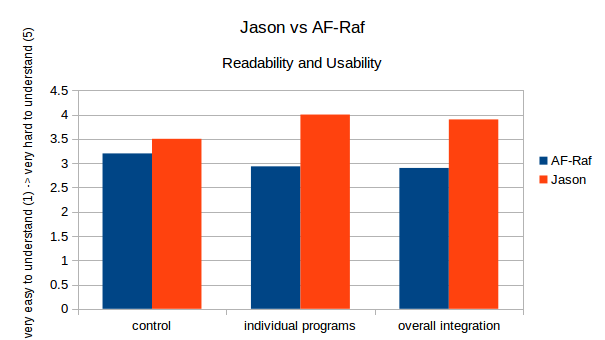
\includegraphics{jasonvsafraf.png}
\caption{Readability and Understanding -- survey results}
\label{fig:Survey}
\end{figure} % >>>

Figure~\ref{fig:Survey} shows a graphical representation of the data.

As the results show, there is a marked decrease in difficulty and a
significant increase in readability and understanding in programs written
in AF-Raf compared to the ones written in Jason. This supports and verify
our hypothesis that the readability and usability of an agent oriented
programming language is improved by the addition of the role and session
programming constructs as well as by the algebraic data types and the type
checking functionality.

% >>>
\chapter{Results and Evaluation}\label{ch:results} % <<<

Our first hypothesis, \textbf{that the integration of roles, based on
sociological Role Theory, will improve the readability and usability of
Agent Oriented Programming languages}, and the corresponding objective:

\begin{itemize}
  \item (1a) \textit{to develop a novel Agent Oriented Programming language that employs roles, based on the existing Agent Factory framework, in order to show how the concept of role maps to a programming language construct in the specific context of Agent Oriented Programming} 
\end{itemize}
were recurrently addressed within this thesis. 

The objective (1a) was achieved by designing (\autoref{sec:roles}),
defining (\autoref{sec:langdef.syntax}, \autoref{sec:opsem}), and
developing (\autoref{ch:casestudy}) roles in AF-Raf with consideration for
readability and usability. Syntactic sugar (\autoref{sec:sugar}) played an
important role in achieving the desired level of readability and
understanding.

The results were evaluated through a number of case
studies (\autoref{ch:casestudy}) and an end-user
survey (\autoref{ch:survey}) that confirmed the initial hypothesis.

The second hypothesis \textbf{that by applying concepts
that had been proved useful, within mainstream programming paradigms, to
Agent Oriented Programming will improve the efficiency and increase
the functionality of the Agent Oriented Programming languages} and its
corresponding objectives were addressed as follows.

\begin{itemize}
  \item (2a) \textit{The first objective, to explore the analogy between Agent
    Oriented Programming languages and Functional Programming languages,
    identify valuable concepts and incorporate them into our new agent
  oriented programming language.} was addressed in (\autoref{sec:roles}).
\item (2b) \textit{The second objective, to investigate the similarity between
    the agent interaction in multiagent systems and the communication
    patterns defined as multiparty session types, and show how the
    multiparty session types can be integrated into our new agent oriented
  programming language.} was addressed in (\autoref{sec:sessions})
\item (2c) \textit{The third objective is to develop a consistent type system,
    and design the first agent oriented programming language to introduce
  type checking.} was addressed in (\autoref{sec:types})
\end{itemize}

Figure~\ref{fig:newFunct} presents what mainstream programming concepts we've applied to AF-Raf and the corresponding new functionality added to AF-Raf
based on this analogy. All new functionality was properly formalised in
(\autoref{sec:langdef.syntax} and \autoref{sec:opsem}).

How were objectives (2a, 2b, 2c) achieved and the second hypotheses
confirmed? It is now clear that the functionality was increased by three
new functionalities: (1) \textbf{roles} that represent a blueprint for
related behaviour, (2) \textbf{sessions} that represent a pattern for agent
communication, and the (3) \textbf{type system} and \textbf{type checking},
which also increase the efficiency of the programming language by
increasing its reliability (errors caught early means less errors at
runtime which in turn leads to more reliability).

The efficiency could be further tested to include evaluation of the speed,
algorithmic efficiency and resource consumption.

\begin{figure}\footnotesize % <<<
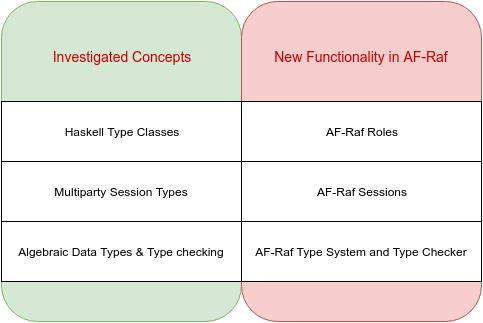
\includegraphics{NewFunctionality.png}
\caption{AF-Raf's New Functionality}
\label{fig:newFunct}
\end{figure} % >>>


% >>>
% >>>

\bookmarksetup{startatroot}
\chapter{Conclusions}\label{ch:conc} % <<<

%\todo{1. Add a chapter to describe the implementation (to include integration
%with Agent Factory and IDE). 2. Add stdio.h to Annex.}

Starting from high-level similarities between certain aspects of an
agent-oriented programming language (2APL) and a functional programming
language (Haskell), we described three new features that could be
particularly helpful for the agent oriented programming languages:
(1)~algebraic data types, which constrain the content of messages,
(2)~roles, which constrain how particular agents interact, and
(3)~sessions, which describe slices of the global interactions in the agent
system. Together, these \emph{language features} support organisational
concepts, which are so far discussed mostly in the literature on
agent-oriented methodologies and frameworks.

The ultimate aim is to provide programmers with a wider set of options at
their disposal for structuring large agent systems. For example, they can
use existing methodologies during the design phase and they can use a
mixture of our proposed language features and existing organisational
frameworks during the implementation phase. First-class language support
has at least two advantages over organisational frameworks. First,
implementations tend to be shorter and more readable. Second,
implementations have stronger correctness guarantees because of the extra
type-checking. On the other hand, organisational frameworks may be
preferred when one needs to interact with legacy code.

The new agent oriented programming language, AF-Raf, based on the existing
Agent Factory framework, implements the innovative features that have been
identified. AF-Raf has types, including algebraic data types, which are
used to constrain the content of the messages. It has type checking, a
feature very useful in identifying programming errors early on. It has
roles, which organise agent behaviour, promoting encapsulation and reuse.
It also have sessions, which further organise agent interaction at a higher
level, namely at the social level. A case study is used to illustrate the
results. The AF-Raf programming language is properly formalised, with its
grammar specified in EBNF format and its operational semantics is defined,
using the small-step operational semantics, as a set of inference rules.

I believe that the research results confirmed our working hypotheses:

\begin{itemize}
\item \textit{The integration of roles improved the readability and
usability of the Agent Oriented Programming languages}. Our objective to
show how the concept of role maps to a programming language construct in
the specific context of Agent Oriented Programming was achieved by
implementing roles \autoref{sec:roles}, as first order constructs, in our new AF-Raf
agent oriented programming language, which was properly formalised in
\autoref{ch:langdef}.

\item \textit{Applying concepts from mainstream programming, like the ones
  of type classes, session types, type checking and algebraic data types,
improved the efficiency and increased the functionality of Agent Oriented
Programming Languages}. Our first objective was achieved by incorporating
the concept of type classes from functional programming into AF-Raf
programming language \autoref{sec:roles}. The second objective was achieved
by incorporating multiparty session types into Af-Raf programming language
\autoref{sec:sessions}. The third objective was achieved by designing a
type system and a type checker that include algebraic data types for AF-Raf
programming languge \autoref{sec:types}.

\end{itemize}
% >>>
\newpage
\appendix
\chapter{Questionnaire type A}\label{app:SurveyA} % <<<
\begin{verbatim}
Questions

Q1. Describe in a few sentences what do you think that the code
in Figure 1.1 does.

Q2. How easy is it for you to read the code in Figure 1.1? Circle
as appropriate.

 very easy
 easy
 neither easy or hard
 hard
 very hard

include stdio
rule Monitoring(name, addr) {
  send(agentID(name, addr), request(status()));
}
rule Message(other, status(alive())) {
  send(other, request(status()));
}
rule Message(other, status()) {
  send(other, inform(status(alive())));
}

Figure 1.1: Monitoring

Q3. Describe in a few sentences what do you think that the
code in Figure 1.2 does.

type conditions = conditions(integer);
type task = increase(integer, integer)
| decrease(integer, integer);
type request = request(task, conditions, deadline(integer));
type bid = bid(integer);
type decision = win() | lose();
type result = failure() | success(integer);
role Buyer {
  ask : request -> bid;
  commit : decision -> result;
}
role Seller {
  sell : request -> result;
}
session BidRound(owner, s : Seller, b1 : Buyer, b2 : Buyer) {
  request : owner -> s;
  request : s -> b1;
  request : s -> b2;
  oneof
  { bid : b1 -> s; win() : s -> b1; result : b1 -> s; }
  { maybe bid : b1 -> s; lose() : s -> b1; };
  oneof
  { bid : b2 -> s; win() : s -> b2; result : b2 -> s; }
  { maybe bid : b2 -> s; lose() : s -> b2; };
  result : s -> owner
}

Figure 1.2: Types, Roles and Sessions

Q4. How easy is it for you to read the code in Figure 1.2? Circle
as appropriate.

 very easy
 easy
 neither easy or hard
 hard
 very hard

Q5. Describe in a few sentences what do you think that the
code in Figure 1.3 does.

include stdio
include ContractNet
action dec(x, y) = raftest.IntegerDecreaseAction;
action inc(x, y) = raftest.IntegerIncreaseAction;
action mul(x, y) = raftest.IntegerMulAction;
agent ContractNetBuyer : Buyer {
  operation ask(request(task, conditions(y), deadline(z)))
  when Multiplier(m) {
    +LastTask(sid, task);
    return bid(mul(m, y));
  }
  operation commit(win())
  when LastTask(sid, decrease(x, y)) {
    return success(dec(x, y));
    -LastTask(sid, decrease(x,y))
  }
  when LastTask(sid, increase(x, y)) {
    return success(inc(x, y));
    -LastTask(sid, increase(x, y));
  }
}

Figure 1.3: Buyer

Q6. How easy is it for you to read the code in Figure 1.3? Circle
as appropriate.

 very easy
 easy
 neither easy or hard
 hard
 very hard

Q7. Describe in a few sentences what do you think that the
code in Figure 1.4 does.

Q8. How easy is it for you to read the code in Figure 1.4? Circle
as appropriate.

 very easy
 easy
 neither easy or hard
 hard
 very hard

include stdio
include ContractNet
agent ContractNetSeller(b1 : Buyer, b2 : Buyer): Seller {
  operation sell(r) {
    if b1.ask(r) < b2.ask(r) then {
      b2.commit(lose());
      return b1.commit(win());
    }
    else {
      b1.commit(lose());
      return b2.commit(win());
    }
  }
}

Figure 1.4: Seller

Q9. How easy is it for you to understand how the three pieces
of code presented in Figure 1.2, Figure 1.3, and Figure 1.4 fit
together? Circle as appropriate.

 very easy
 easy
 neither easy or hard
 hard
 very hard

Circle as appropriate:

Q10. Gender.

 Male
 Female

Q11. Age range.

 <25
 25-35
 >35

Q12.Years of programming experience in a payed job.

 <3
 3-10
 >10

Q13. Number of years since you first started programming.
 
 <5
 5-10
 >10

Q14. Number of programming languages you are proficient in.

 1
 2-3
 >3

Q15. Level of familiarity with Functional languages.

 very familiar
 familiar
 basic familiarity
 know almost nothing about them

Q16. Level of familiarity with Object Oriented Programming
languages.
 
 very familiar
 familiar
 basic familiarity
 know almost nothing about them

 Q17. Level of familiarity with Agent Oriented Programming
languages.
 
 very familiar
 familiar
 basic familiarity
 know almost nothing about them

 Q18. Last level of qualification in Computer Science.

less than Bachelor Degree
 Bachelor Degree
 Postgraduate level
\end{verbatim}

% >>>

\chapter{Questionnaire type B}\label{app:SurveyB} % <<<
\begin{verbatim}
Questions

Q1. Describe in a few sentences what do you think that the code
in Figure 1.1 does.

Q2. How easy is it for you to read the code in Figure 1.1? Circle
as appropriate.

 very easy
 easy
 neither easy or hard
 hard
 very hard

+monitoring(?name, ?addr) : true <-
.send(request, agentID(?name, ?addr), status);
+message(inform, agentID(?name, ?addr), status(alive)) :
monitoring(?name, ?addr2) <-
.send(request, agentID(?name, ?addr), status);
+message(request, ?sender, status) : true <-
.send(inform, ?sender, status(alive));

Figure 1.1: Monitoring

Q3. Describe in a few sentences what do you think that the
code in Figure 1.2 does.

price(Task,X) :- .random(R) & X = (10*R)+100.
plays(initiator,c).
+plays(initiator,In)
: .my_name(Me)
<- .send(In,tell,introduction(participant,Me)).
@c1 +cfp(CNPId,Task)[source(A)]
: plays(initiator,A) & price(Task,Offer)
<- +proposal(CNPId,Task,Offer);
.send(A,tell,propose(CNPId,Offer)).
@r1 +accept_proposal(CNPId)
: proposal(CNPId,Task,Offer)
<- .print("My proposal ’",Offer,"’ won CNP ",CNPId,
" for ",Task,"!").
@r2 +reject_proposal(CNPId)
<- .print("I lost CNP ",CNPId, ".");
-proposal(CNPId,_,_).

Figure 1.2: Participant

Q4. How easy is it for you to read the code in Figure 1.2? Circle
as appropriate.

 very easy
 easy
 neither easy or hard
 hard
 very hard

Q5. Describe in a few sentences what do you think that the
code in Figure 1.3 does.

Q6. How easy is it for you to read the code in Figure 1.3? Circle
as appropriate.

 very easy
 easy
 neither easy or hard
 hard
 very hard

all_proposals_received(CNPId) :-
.count(introduction(participant,_),NP) &
.count(propose(CNPId,_), NO) &
.count(refuse(CNPId), NR) &
NP = NO + NR.
!startCNP(1,fix(computer_123)).
+!startCNP(Id,Object)
<- .wait(2000);
+cnp_state(Id,propose);
.findall(Name,introduction(participant,Name),LP);
.print("Sending CFP to ",LP);
.send(LP,tell,cfp(Id,Object));
.concat("+!contract(",Id,")",Event);
.at("now +4 seconds", Event).
@r1 +propose(CNPId,Offer)
: cnp_state(CNPId,propose) & all_proposals_received(CNPId)
<- !contract(CNPId).
@r2 +refuse(CNPId)
: cnp_state(CNPId,propose) & all_proposals_received(CNPId)
<- !contract(CNPId).
@lc1[atomic]
+!contract(CNPId)
: cnp_state(CNPId,propose)
<- -+cnp_state(CNPId,contract);
.findall(offer(O,A),propose(CNPId,O)[source(A)],L);
.print("Offers are ",L);
L \== [];
.min(L,offer(WOf,WAg));
.print("Winner is ",WAg," with ",WOf);
!announce_result(CNPId,L,WAg);
-+cnp_state(Id,finished).
@lc2 +!contract(CNPId).
-!contract(CNPId)
<- .print("CNP ",CNPId," has failed!").
+!announce_result(_,[],_).
+!announce_result(CNPId,[offer(O,WAg)|T],WAg)
<- .send(WAg,tell,accept_proposal(CNPId));
!announce_result(CNPId,T,WAg).
+!announce_result(CNPId,[offer(O,LAg)|T],WAg)
<- .send(LAg,tell,reject_proposal(CNPId));
!announce_result(CNPId,T,WAg).

Figure 1.3: Initiator

Q7. How easy is it for you to understand how the two pieces of
code presented in Figure 1.2 and Figure 1.3 fit together? Circle as
appropriate.

 very easy
 easy
 neither easy or hard
 hard
 very hard

Circle as appropriate:

Q8. Gender.

 Male
 Female

Q9. Age range.

 <25
 25-35
 >35

Q10.Years of programming experience in a payed job.

 <3
 3-10
 >10

Q11. Number of years since you first started programming.

 <5
 5-10
 >10

Q12. Number of programming languages you are proficient in.

 1
 2-3
 >3

Q13. Level of familiarity with Functional languages.

 very familiar
 familiar
 basic familiarity
 know almost nothing about them

Q14. Level of familiarity with Object Oriented Programming
languages.

 very familiar
 familiar
 basic familiarity
 know almost nothing about them

Q15. Level of familiarity with Agent Oriented Programming
languages.

 very familiar
 familiar
 basic familiarity
 know almost nothing about them

Q16. Last level of qualification in Computer Science.

 less than Bachelor Degree
 Bachelor Degree
 Postgraduate level
\end{verbatim}
% >>>

\chapter{stdio.raf}\label{app:standardLibrary} % <<<

\begin{verbatim}

action println(s) = 
        com.agentfactory.raf.RafStandardAction$Println;

action terminate() = 
        com.agentfactory.raf.RafStandardAction$Terminate;

action send(agentId(name, address), message) =
        com.agentfactory.raf.RafStandardAction$Send;

sensor com.agentfactory.raf.RafStandardSensor$Message;

\end{verbatim}

% >>>

\backmatter
\bibliographystyle{plain}
\bibliography{thesis}
\end{document}
% >>>
% vim:fmr=<<<,>>>:tw=75:spell:fo+=t:
